%\setcounter{section}{2}
\section{国際SKAのサイエンス}\label{c03.s2}
\subsection{$B:FEEN%$NJ*M}(B}\label{c03.s2.ss1}%\label{phys}
\subsubsection{$BF3F~(B}

$B3F>l=j$G$NEEN%EY(B$x_{\rm \textsc{Hii}}$$B$N?J2=$O0J2<$N$h$&$KI=$;$k!#(B
\begin{equation}
\frac{d x_{\rm \textsc{Hii}}}{dt} = k_{\rm col} (T) (1-x_{\rm
 \textsc{Hii}})n_{\rm e} - \alpha(T)x_{\rm \textsc{Hii}} n_{\rm e} +
 k_{\rm ph}(1-x_{\rm \textsc{Hii}}) 
\end{equation}
$B$3$3$G!"(B$k_{\rm col}(T)$$B$O>WFMEEN%N(!"(B$n_{\rm e}$$B$OEE;R?tL)EY!"(B
$\alpha(T)$$B$O:F7k9gN(!"(B$k_{\rm ph}$$B$O8wEEN%N($G$"$k!#8wEEN%N($O!"3FCOE@$G(B
$B$NmU<M6/EY(B$I_\nu$$B$rMQ$$$F!"(B
\begin{equation}
k_{\rm ph}= \int d\Omega \int_{\nu_{\rm L}}^\infty
 \frac{I_\nu}{h\nu}\sigma_\nu d\nu 
\end{equation}
$B$HI=$;$k!#$3$3$G!"(B$\nu_{\rm L}$$B$O%i%$%^%sC<?6F0?t!"(B$\sigma_\nu$$B$OEEN%CGLL(B
$B@Q$G$"$k!#8wEEN%2aDx$O!"%(%M%k%.!<J}Dx<0$H$b%+%C%W%k$9$k0Y!"EEN%?J2=$HF1(B
$B;~$K%(%M%k%.!<J}Dx<0(B
\begin{equation}
\frac{du}{dt} = \frac{\Gamma - \Lambda}{\rho}
\end{equation}
$B$r2r$/I,MW$,$"$k!#$3$3$G!"(B$u$$B$OC10L<ANL$"$?$j$NFbIt%(%M%k%.!<$G$"$k!#$^(B
$B$?!"(B$\Gamma$$B$OC10LBN@Q$"$?$j$N2CG.N(!"(B$\Lambda$$B$OC10LBN@Q$"$?$jNd5QN($G(B
$B$"$j!"$3$l$i$K$O!"8w2CG.!"CGG.2CG.(B($BNd5Q(B)$B!">WFMEEN%Nd5Q!":F7k9gNd5Q!">WFM(B
$BNe5/Nd5Q!"@)F0J|<MNd5Q!"%3%s%W%H%s2CG.(B($BNd5Q(B)$B$J$I$,4^$^$l$k!#FC$K8w2CG.N((B
$B$O!"(B
\begin{equation}
\Gamma_{\rm ph}= n_{\rm \textsc{Hi}}\int d\Omega \int_{\nu_{\rm L}}^\infty \frac{I_\nu}{h\nu}(h\nu-h\nu_{\rm L})\sigma_\nu d\nu
\end{equation}
$B$HI=$;$k!#(B
$BEEN%$5$l$?%,%9$O!"$*$h$=(B10,000-20,000K$B$^$G2CG.$5$l$k(B(e.g.,
\cite{1996ApJ...465..608T})$B!#$3$N2CG.$K$h$j!"=ENO%]%F%s%7%c%k$N@u$$%,%9(B
$B1@$N=ENO<}=L$OAK32$5$l!"9b$$%,%905$K$h$C$F>.$5$J%9%1!<%k$N9=B$$O6Q$5$l$k!#(B
$B$3$N2aDx$r8w>xH/(B(photo-evaporation)$B$H8F$V!#(B

\subsubsection{$BEEN%2aDx$X$NF6;!(B}
\noindent\underline{\bf $BJ?6Q<+M39TDx(B}$B!!1'Ch$G$NEEN%8w;R$NJ?6Q<+M39TDx$O!"(B
\begin{equation}
l = \frac{1}{\sigma_\nu n_{\rm \textsc{Hi}}}\approx 2 \left(\frac{10}{1+z}\right)^2\left(\frac{\nu}{\nu_{\rm L}}\right)^3 \left(\frac{1}{x_{\rm \textsc{Hi}}}\right)\;{\rm comoving\;kpc}
\end{equation}
$BDxEY$G$"$k!#EEN%GHLL$N8|$5$OJ?6Q<+M39TDxDxEY$H$J$k$H9M$($i$l!";g30@~$N>l9g!"J?6Q<+M39TDx$O>.$5$$$?$a!"EEN%GHLL$OHs>o$K%7%c!<%W$K$J$k!#(B
$B0lJ}$G!"(B1keV$B0J>e$N(BX$B@~$NJ?6Q<+M39TDx$O(B$\sim$1 comoving  Gpc$B$H$J$j!"DcEEN%(B
$BEY$+$D0lMM$K6a$$EEN%9=B$$,4|BT$5$l$k!#(B

\noindent\underline{\bf $B:F7k9g;~4V(B}$B!!EEN%%,%9$O!"$*$h$=(B$T=10^4$K$B$KJ]$?$l(B
$B$k!#$3$N$H$-$N:F7k9gN($rMQ$$$F!"1'Ch$NJ?6QL)EY$G$N:F7k9g;~4V$O!"(B 
\begin{equation}
t_{\rm rec} = \frac{1}{\alpha (T)n_{\rm H}}\approx 240 \left(\frac{10}{1+z}\right)^3 {\rm Myr}
\end{equation}
$B$H$J$k!#9b@VJ}JP0\(B($1+z>10$)$B$K$*$$$F!"%_%K%O%m!<$d%U%#%i%a%s%H$J$I$N9=B$(B
($\frac{\delta \rho}{\rho}>20 $)$B$G$O!":F7k9g;~4V$O$*$h$=(B10Myr$B0J2<$H$J$j!"(B
$B$3$N$h$&$J9=B$$O!"8w>xH/$K$h$C$F9=B$$,$J$i$5$l$k$^$G8w;R5[<}BN$H$7$FF/$/(B
\citep{2014MNRAS.440.1662S}$B!#(B 

\noindent\underline{\bf $BM}A[%9%H%m%`%0%l%s5e(B}$B!!0lMML)EY>l$N>l9g!"8w;R8;(B
$B<~$j$NEEN%NN0h$O%9%H%m%`%0%l%s5e$H8F$P$l$k%b%G%k$GI=$;$k!#%9%H%m%`%0%l%s(B
$B5e$N%5%$%:(B($B%9%H%m%`%0%l%sH>7B(B)$B$O!"NN0hFb$G$NC10L;~4V$"$?$j$N:F7k9g?t$HEE(B
$BN%8w;R?t$,D`$j9g$$$K$h$C$F7hDj$5$l!"(B 
\begin{equation}
r_{\rm S} = \left( \frac{3 \dot{N_{i}}}{4\pi n_{\rm H}^2 \alpha_{\rm B} (T)}\right)^{\frac{1}{3}}
\end{equation}
$B$HI=$;$k!#$3$3$G!"(B$\dot N_{i}$$B$OEEN%8w;RJ|<MN(!"(B$\alpha_{\rm B}(T)$$B$OBh0lNe5/>u(B
$BBV0J>e$N=`0L$X$N:F7k9gN($G$"$k!#$3$N%b%G%k$rMQ$$$k$H!"Nc$($P(B$\dot N_{i}=5\times 10^{48}$/s, $n_{\rm H}=10^{-3}\rm cm^{-3}$$B$N$H$-(B$r_{\rm s}\approx
5.4$kpc$BDxEY$H$J$k!#(B

\subsubsection{$B86;O6d2OFb$K$*$$$F:FEEN%$K4XO"$9$k=t2aDx(B}
\noindent\underline{\bf $BEEN%8w;R$NC&=P(B}$B!!6d2O4VJ*<A$NEEN%?J2=$N2rL@$K$O!"(B
$B6d2O$+$iH4$1=P$9EEN%8w;R$NNL$,=EMW$H$J$k!#$3$NNL$O!"FC$K@17A@.N($HEEN%8w(B
$B;R$NC&=P3d9g(B($BC&=P8w;RN((B)$B$KJ,$1$F9M$($k$N$,JXMx$G$"$k!#:FEEN%4|$N8e4|CJ3,(B
$B$G$O!"6d2OFb$N%@%9%H$bC&=P8w;RN($K4X$7$F=EMW$JLr3d$r2L$?$92DG=@-$,$"$k!#(B 

$B4QB,E*$JC&=P8w;RN($r8+@Q$b$j$O!"6d2O4VJ*<A$N6/$$5[<}$K$h$jHs>o$K:$Fq$G$"(B
$B$k$,!"(B$z\approx3$$B$G$OD>@\E*$KEEN%8w;R$,8!=P$5$l$F$*$j!"?t%Q!<%;%s%H$+$i(B
$B?t(B10$B%Q!<%;%s%H$NCM$,<($5$l$F$$$k(B (e.g., \cite{2001ApJ...546..665S,
2009ApJ...692.1287I})$B!#$h$j9b@VJ}JP0\6d2O$K$D$$$F$O!"$$$/$D$+$N2>Dj$N4p(B
$B$E$-!"C&=P8w;RN($K>e8B(B($B@VJ}JP0\(B$z=5.7$$B$G(B$\sim60$$B%Q!<%;%s%H(B)$B$rM?$($?8&5f(B
$B$,$"$k(B (e.g.,\cite{2010ApJ...724.1524O})$B!#4QB,$5$l$k6d2O$N8D?tL)EY$+$i$O!"(B
$B@1$,:FEEN%$N<g$J8w;R8;$G$"$k>l9g!"9b@VJ}JP0\$[$I9b$$C&=P8w;RN(!"$"$k$$$O(B
$BDc<ANL6d2O$[$I9b$$C&=P8w;RN($G$J$$$H%H%`%=%s;6Mp$N8w3XE*8|$_$N4QB,7k2L$r(B
$BK~$9$3$H$,:$Fq$G$"$k$H<(:6$5$l$k(B (e.g., \cite{2012ApJ...759L..38A,
2012ApJ...746..125H, 2012MNRAS.419.1480M})$B!#(B 

$BM}O@E*$K$O!"<g$K?tCM%7%_%e%l!<%7%g%s$K$h$C$FC&=P8w;RN($,D4$Y$i$l$F$$$k(B
(e.g., \cite{2008ApJ...672..765G, 2009ApJ...693..984W,
2010ApJ...710.1239R, 2011MNRAS.412..411Y, 2013MNRAS.429L..94P,
2014MNRAS.442.2560W})$B!#$3$l$i$N7W;;7k2L$O!"J,2rG=$N0c$$!"%b%G%k$N0c$$$J(B
$B$I$+$iDjNLE*$K$OCM$,<}B+$7$F$$$J$$$,!"C&=P8w;RN($NDj@-E*$J?6$kIq$$$H$7$F(B
1) $B%O%m!<<ANL$,Bg$-$$$[$I>.$5$$!"(B2) $B9b@VJ}JP0\$[$IBg$-$$!"$H$$$&7k2L$,B?(B
$B$$!#(B 

\noindent\underline{\bf $B86;O6d2O$G$NmU<M@-%U%#!<%I%P%C%/(B}$B!!8w2CG.$dmU<M(B
$B05$H$$$C$?%U%#!<%I%P%C%/$O!"6d2OFb$N%,%9$d6d2O$X9_Ce$9$k%,%9!"6d2O4V%,%9(B
$B$N%@%$%J%_%/%9$K1F6A$rM?$($k(B (e.g., \cite{2009MNRAS.400.1283I,
2012MNRAS.427..311W, 2012MNRAS.424..377D, 2013MNRAS.428..154H}) $B!#(B
$B$3$N8z2L$O!"@17A@.N($N$_$J$i$:>e5-$NC&=P8w;RN($K$b1F6A$rM?$((B
$B$k;v$,<($5$l$F$$$k(B (e.g., \cite{2009ApJ...693..984W,
2012PTEP.2012aA306U})$B!#$^$??eAGJ,;R$N2rN%8w;R$O!"1'Ch=i4|$N<g$?$kNd5Q:`(B
$B$G$"$k?eAGJ,;R$r2rN%$9$k$?$a!"$3$N2aDx$b@17A@.N($K1F6A$rM?$($k!#$3$l$i(B
$BmU<M@-%U%#!<%I%P%C%/$rE,@Z$K9MN8$9$k;v$O!"6d2O$+$i$NEEN%8w;R6!5kNL$rL@$i(B
$B$+$K$9>e$GHs>o$K=EMW$G$"$k!#(B 

\subsubsection{$B6d2O4VJ*<A$G$NEEN%2aDx(B}
\noindent\underline{\bf $BEEN%GHLL$NH/E8(B}$B!!(B
$B0lMM$+$DDj>o$JL)EY>l$N>l9g!"EEN%GHLL$NH/E8$O!"EEN%GHLL$G$NEEN%8w;R%U%i%C(B
$B%/%9$HEEN%%,%9%U%i%C%/%9$ND`$j9g$$$+$i!"%9%H%m%`%0%l%sH>7B(B$r_{\rm S}$$B!"(B
$B:F7k9g;~4V(B$t_{\rm rec}$$B$rMQ$$$F(B
\begin{equation}
r_{\rm I} = r_{\rm S}[1- \exp(-t/t_{\rm rec})]^{\frac{1}{3}}
\end{equation}
$B$HI=$;$k(B \citep{Spitzer78} $B!#$b$7!"9bL)EY%,%92t$,B8:_$9$k>l9g!"$3$N%,%9(B
$B2t$,8w>xH/$5$l$J$$8B$j!"EEN%GHLL$O%,%92tFb$KJa$o$l$k(B ($B?^(B\ref{KH1})$B!#(B\\

\underline{{\bf X$B@~$K$h$kEEN%$H2CG.(B}}$B!!(BX$B@~$OM-8z$JEEN%8w;R8;$G$"$k$,!";g(B
$B30@~$H$O0[$J$j(BX-ray$B$OJ?6Q<+M39TDx$,Bg$-$$0Y!"1'ChKDD%$K$h$k?6F0?t$NJQ2=(B
$B$r9MN8$9$kI,MW$,$"$k!#$^$?!"8D!9$N8w;R$,$b$D%(%M%k%.!<$,9b$$0Y!"EEN%$N:](B
$B$KHt$S=P$9EE;R$K$h$kFs<!E*$J>WFMEEN%(B(secondary ionization)$B$N8z2L$b9MN8$9(B
$B$kI,MW$,$"$k(B (e.g.,\cite{2010A&A...523A...4B})$B!#(B 

%figure moved to ss2
%再電離の物理
\subsection{$B:FEEN%4|$N%b%G%j%s%0$H(BSKA$B$X8~$1$?%7%_%e%l!<%7%g%s(B}\label{c03.s2.ss2}%\label{EoRSim}

\begin{figure}[!t]
	\centering
	{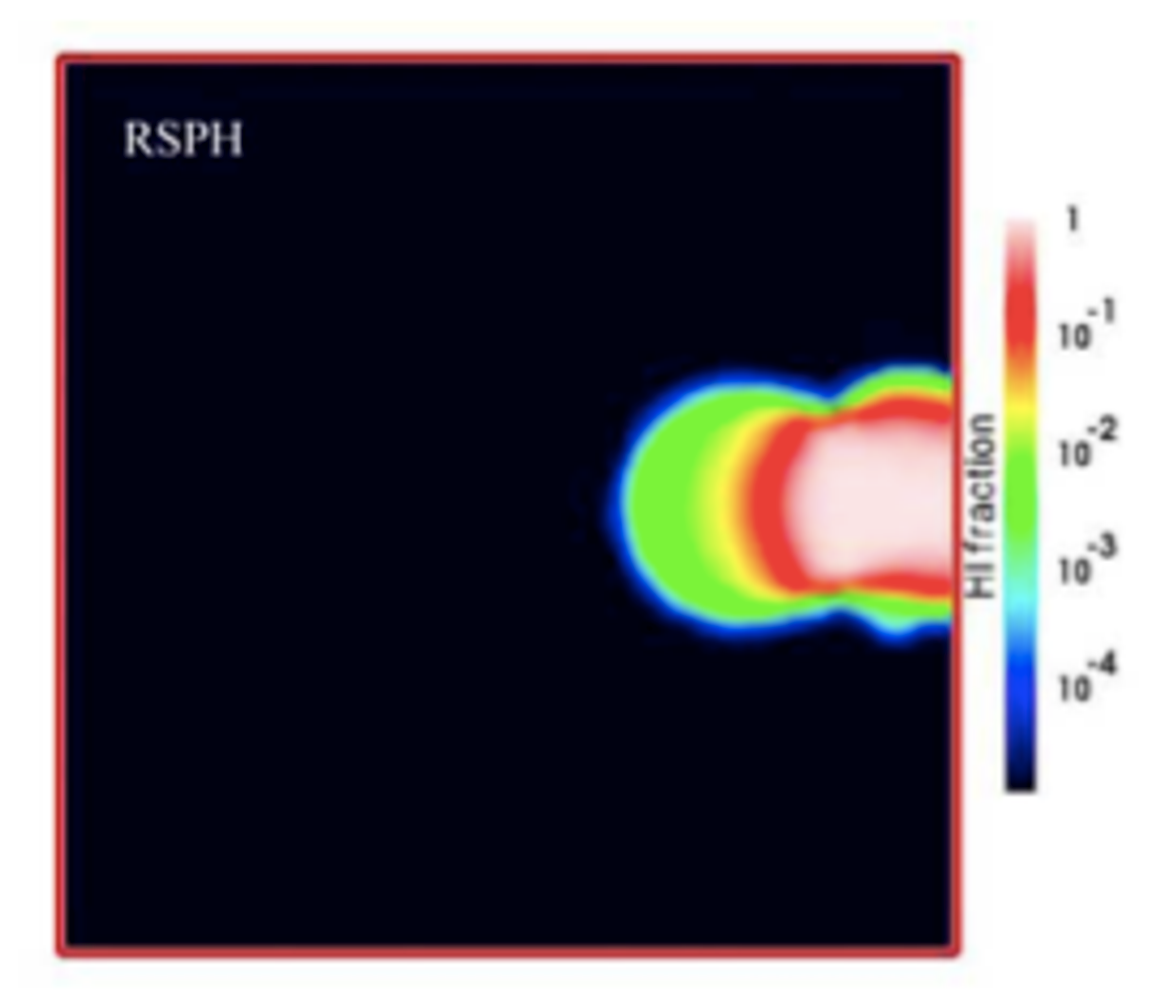
\includegraphics[width=7.5cm]{EoR/c03/c03.s2.f1a.eps}}
	{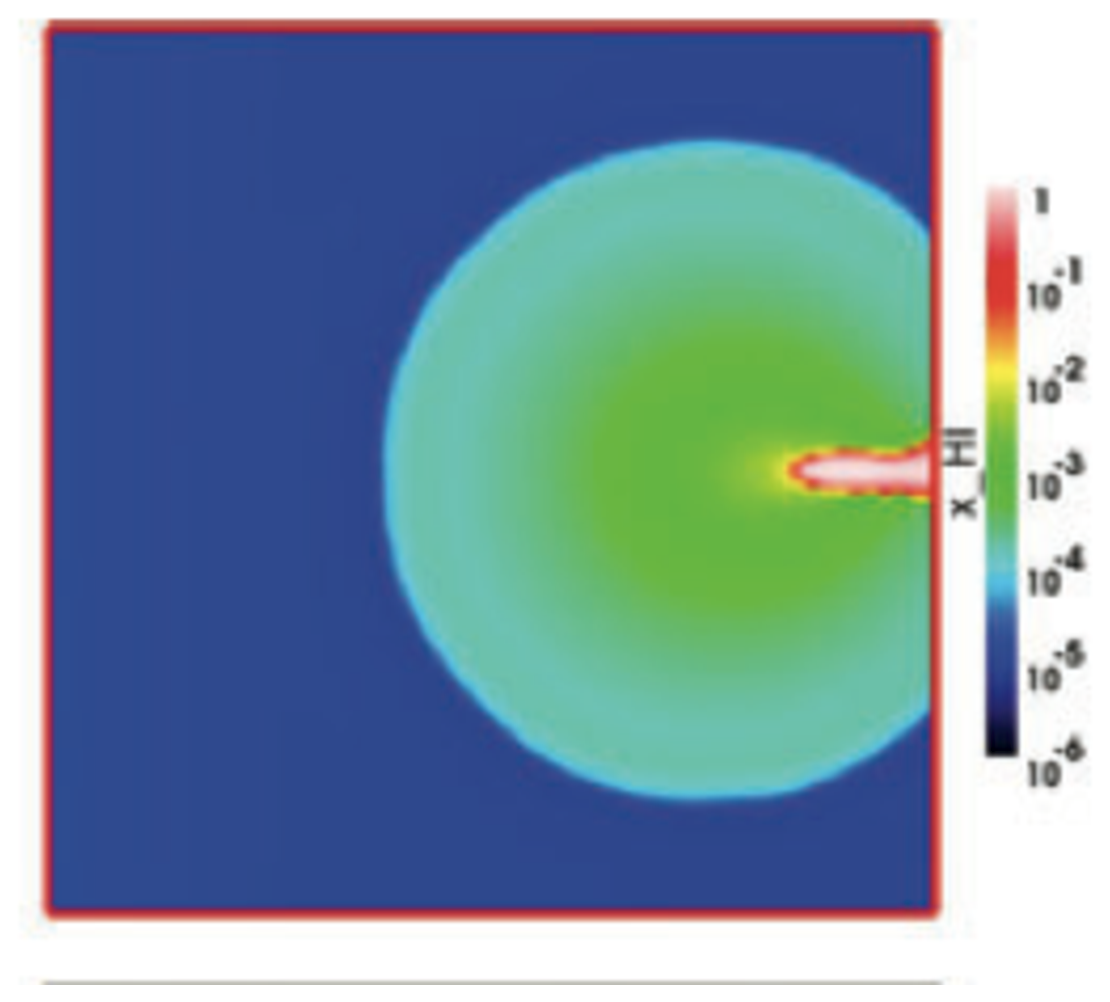
\includegraphics[width=7.5cm]{EoR/c03/c03.s2.f1b.eps}}
	\caption{$B:8$+$i0lMMEEN%8w;R%U%i%C%/%9$,9bL)EY%,%92t$KF~<M$9$k>l9g$N7W;;7k2L(B(\cite{2009MNRAS.400.1283I}, RSPH$BK!$K$h$k7W;;7k2L$rH4?h(B)$B!#:8?^!'@EE*$J%,%9$N>l9g!"EEN%GHLL$O%,%92t$KJa$o$l$k!#1&?^!'F0E*$J%,%9$N>l9g!"%,%92t$O8w>xH/$7!"EEN%GHLL$,?J$`$h$&$K$J$k!#(B}\label{KH1}
\end{figure}
\begin{figure}[!h]
	\centering {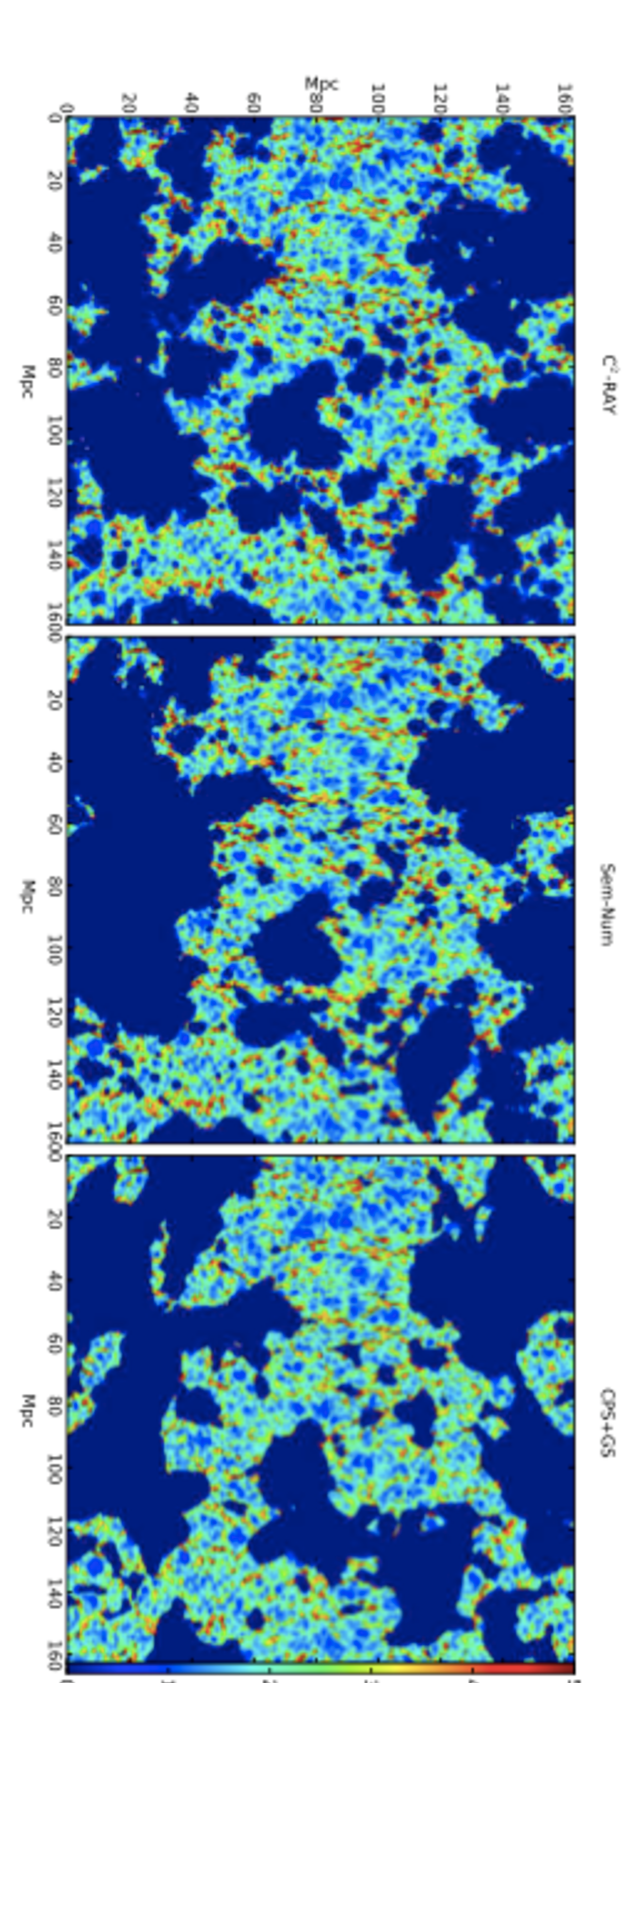
\includegraphics[width=0.3\linewidth,
	angle=90]{EoR/c03/c03.s2.f2.eps}} 
\caption{$BmU<MM"Aw%7%_%e%l!<%7%g%s(B($B:8?^(B)$B!"%O%m!<J,I[$rMQ$$$?=`?tCME*:FEEN%(B
	$B%7%_%e%l!<%7%g%s(B($BCf1{?^(B)$B!"(BPress-Schechter$B$rMQ$$$?=`?tCME*:FEEN%%7(B
	$B%_%e%l!<%7%g%s(B($B1&?^(B)$B$K$h$k(B21 cm$B@~6/EYJ,I[$NHf3S!#%O%m!<J,I[$rMQ$$$?(B
	$B=`?tCME*:FEEN%%7%_%e%l!<%7%g%s$G$O!"mU<MM"Aw%7%_%e%l!<%7%g%s$N(B21 cm
	$B@~6/EYJ,I[(B
	$B$r$h$/:F8=$G$-$k$,!"(BPress-Schechter$B$rMQ$$$?=`?tCME*:FEEN%%7(B
	$B%_%e%l!<%7%g%s$G$O!"mU<MM"Aw%7%_%e%l!<%7%g%s$N:F8=@-$OMn$A$k(B
	$B$3$H$,$o$+$k!#(B
	\citep{2014MNRAS.443.2843M}$B!#(B}\label{KH6}
\end{figure}
SKA$B$K$h$k@VJ}JP0\$7$?(B21 cm$B@~4QB,$G$O!":FEEN%4|$d$=$l0JA0$N;~4|$K$*$1$k(BIGM
$B$N(B3$B<!85%H%b%0%i%U%#!<$,F@$i$l$k$H4|BT$5$l$k!#<B:]$K4QB,$5$l$k$G$"$m$&(B
21 cm$B%7%0%J%k$O:FEEN%$NHs0lMM@-$K5/0x$9$k%Q%?!<%s$K4XO"$7$?Hs>o$KBg$-$J%9(B
$B%1!<%k$N$b$N$G$"$k$N$KBP$7!"2f!9$,CN$j$?$$$N$O!"=iBe6d2O$N$h$&$KHs>o$K>.(B
$B$5$/0E$$E7BN$N>pJs$G$"$k0Y!"$=$3$K$OBg$-$J3V$?$j$,B8:_$9$k!#=iBe6d2O$NFC(B
$BD'(B (Spectral Energy Distribution: SED$B!"8D?tEy(B) $B$N4QE@$+$i!"4QB,$5$l$k(B21
cm$B%7%0%J%k$r2r<a$9$k:]$K$O!"$3$l$i$N>\:Y$J%b%G%j%s%0$,=EMW$H$J$k!#(B 


$B6aG/$N:FEEN%%b%G%j%s%0$G$O!"<g$KD>@\E*$J?tCM%7%_%e%l!<%7%g%s$d=`2r@OE*(B/$B=`(B
$B?tCME*(B(semi-analytic/semi-numerical)$B%b%G%j%s%0(B
\citep{2004ApJ...613...1F, 2005ApJ...630...657Z, 2009ApJ...703L.167A,
2007ApJ...663..693M,2009MNRAS.394..960C,2010MNRAS.406..2421S}$B$,MQ$$$i$l$k!#(B



\subsubsection{$B8=B8$9$k%b%G%j%s%0$NMW;](B}
\noindent\underline{\bf $B%7%_%e%l!<%7%g%s(B}$B!!%7%_%e%l!<%7%g%s$O!"Bg$-$/(B2$B$D(B
$B$N%?%$%W$KJ,$1$i$l$k!#$R$H$D$O!">.7W;;NN0h$+$D9bJ,2rG=$N%7%_%e%l!<%7%g%s(B
$B$G$"$j!"$3$l$K$h$j6d2O7A@.$K$*$1$kmU<M$dD6?7@1GzH/$K$h$k%,%9$X$N%U%#!<%I%P%C%/(B
$B$r>\:Y$K8&5f$G$-$k$,!"Bg6IE*$J:FEEN%$d$=$N4QB,E*:/@W$rI=8=$9$k$N$K$O7W;;(B
$BNN0h$,IT==J,$G$"$k(B\citep{1997ApJ...486...581G,2000MNRAS.314..611C, 2002ApJ...575..33R}$B!#$b$&0l$D$O!"Bg$-$J7W;;NN0h$G$N(B
$B%7%_%e%l!<%7%g%s$G$"$j!">.%9%1!<%k$NJ*M}$OJ,2r$G$-$J$$JQ$o$j$K!"%0%m!<%P(B
$B%k$J:FEEN%?J2=$r8&5f$G$-$k(B\citep{2006MNRAS.369..1625I,2014MNRAS.439..725I})$B!#$3$N>l9g!"J,2r$G$-$F$$$J$$%9%1!<%k$K$O!"9bJ,2rG=$N(B
$B7W;;7k2L$dB>$N%b%G%j%s%0$K$h$k%5%V%0%j%C%I%b%G%k(B
\footnote{$B%7%_%e%l!<%7%g%s$N6u4VJ,2rG=(B($B%0%j%C%I%5%$%:(B)$B$OM-8B$G$"$j!"(B
$B$7$P$7$P6u4VJ,2rG=0J2<$N%9%1!<%k$N;v>]!"9=B$Ey$r@5$7$/DI$($J$$(B
$B;v$,$"$k!#$3$N$H$-!"6u4VJ,2rG=0J2<(B($B%0%j%C%I%5%$%:0J2<(B)$B$NItJ,$K2>Dj$9$k(B
$B%b%G%k$N;v$r%5%V%0%j%C%I%b%G%k$H8F$V!#(B}
$B$rMQ$$$k(B\citep{2007MNRAS.376..534I, 2007MNRAS.377..1043M, 2012ApJ...756L..16A}$B!#(B

\noindent\underline{\bf $B=`2r@OE*(B/$B=`?tCME*%b%G%j%s%0(B}$B!!(BEoR$B$N%b%G%j%s%0$K$O!"(B
2$B$D$N:$Fq$,$"$k!#0l$D$O!"9-$$%@%$%J%_%C%/%l%s%8(B\footnote{$BNc$($P!"6d2OFb$N(B
$B@17A@.$d$=$l$i$K$h$k%U%#!<%I%P%C%/$O(Bkpc$B0J2<$N%9%1!<%k$N8=>]$G$"$j!"1'ChO@(B
$BE*%9%1!<%k$NEEN%9=B$$dJ*<AJ,I[$r8+$h$&$H;W$($P(B0.1-1Gpc$B$,I,MW$G$"$k!#(B}$B$G$"(B
$B$j!"$7$P$7$P%5%V%0%j%C%I%b%G%k$,I,MW$H$J$k!#$b$&0l$D$O!"2f!9$,9b@VJ}JP0\(B
$B$NE7BN7A@.;K$d$=$l$iE7BN$NFCD'$r==J,$K2rL@$G$-$F$$$J$$;v$K5/0x$9$k9-$$%Q(B
$B%i%a!<%?%9%Z!<%9$G$"$j!"%5%V%0%j%C%I%b%G%k$rE,MQ$9$k$H$7$F$b$3$NLdBj$O;D(B
$B$k!#$3$l$i:$Fq$r9nI~$9$k$?$a!"6aG/$G$ODc7W;;%3%9%H$G<B9T2DG=$J=`?tCME*:F(B
$BEEN%%7%_%e%l!<%7%g%s(B (semi-numerical EoR simulation) $B$H8F$P$l$k<jK!$,H/C#$7(B
$B$?!#(B

$B=`?tCME*:FEEN%%7%_%e%l!<%7%g%s$N4pK\E*$JFCD'$O!$mU<MM"Aw7W;;$rD>@\2r$/$H(B
$B$$$&2aDx$r!"EEN%8w;R?t$H86;R?t(B($B$7$P$7$P:F7k9gN($K$h$kJd@5$,$5$l$k(B)$B$NHf3S(B
$B$K$h$C$FEEN%H=Dj$r9T$&$H$$$&6a;wE*$J<h$j07$$$KCV$-49$($kE@$G$"$k(B
 \citep{2006MNRAS.365..115F}$B!#J|<M8;$NJ,I[$K$O!"(B$N$-$BBN%7%_%e%l!<%7%g%s$GF@(B
$B$i$l$?J,I[$rMQ$$$k>l9g$d(B \citep{2007ApJ...654...12Z,
2009MNRAS.394..960C}$B!"9bB.$J%<%k%I%S%C%A6a;w$J$I$rMQ$$$k>l9g$,$"$k(B
 \citep{2007ApJ...663..693M}\footnote{$B=`?tCME*:FEEN%7W;;%3!<%I$N0lNc$G$"(B
$B$k(B21 cmFAST \citep{2011MNRAS.411..9551M}$B$K$D$$$F$O!"(B\ref{c03.s3.ss1}$B@a(B
$B$r;2>H!#(B}$B!#(B 
$B$3$l$i=`?tCME*:FEEN%%7%_%e%l!<%7%g%s7k2L$H!"D>@\mU<M(B
$BM"Aw$r2r$/;v$GEEN%9=B$$rF@$kmU<MM"Aw%7%_%e%l!<%7%g%s7k2L$NHf3S$O9-$/9T$o(B
$B$l$F$-$F$*$j(B\citep{2011MNRAS.414..727Z, 2014MNRAS.443.2843M}$B!"(BMpc
$B%9%1!<%k0J>e$G$ONI$/0lCW$9$k$H8@$o$l$F$$$k$,!"8e=R$9$k$h$&$K$h$j>\:Y$J2a(B
$BDx$r4^$a$?7W;;$G$NHf3S$OI,MW$G$"$m$&!#(B
%Majumdar et al. (2014) 
\citet{2014MNRAS.443.2843M}
$B$G$O!"mU<MM"Aw(B
$B%7%_%e%l!<%7%g%s$HF1$8%O%m!<$NJ,I[$rD>@\;H$C$?=`?tCME*:FEEN%%7%_%e%l!<%7%g(B
$B%s$O!"mU<MM"Aw%7%_%e%l!<%7%g%s$K$h$C$FF@$i$l$k(B$k<1.0 {\rm Mpc^{-1}}$$B$N%9(B
$B%1!<%k$G$NEEN%;K$r(B90\%$B0J>e$N@53N$5$G:F8=$G$-$k$H$7$F$$$k!#0lJ}$G!"%O%m!<(B
$B$NJ,I[$rMQ$$$:$K(BPress-Schechter formalism$B$rMQ$$$?>l9g!"F1$8%9%1!<%k$G$N:F(B
$B8=@-$O(B$>$40\%$B$^$GMn$A$k$b$N$N!"J?6QE*$JEEN%;K$J$I$OmU<MM"Aw%7%_%e%l!<%7%g(B
$B%s$H$*$*$h$=0lCW$9$k(B ($B?^(B\ref{KH6})$B!#(B

$B$3$N$h$&$JHf3S7k2L$O!":FEEN%$N%7%J%j%*$d%b%G%j%s%0$N;EJ}$K$h$C$F$bJQ$o$k(B
$B$H;W$o$l$k!#:FEEN%;K$d(B21 cm$B%7%0%J%k$NFCD'$OMM!9$JMW0x$K$h$C$F3F;~4|$G0[$J(B
$B$k!#$=$N0l$D$NMW0x$OmU<M@-%U%#!<%I%P%C%/$K$h$kDc<ANL6d2O$G$N@17A@.AK32$G(B
$B$"$k(B(\ref{c03.s2.ss1}$B@a$r;2>H(B)$B!#$3$N8z2L$O!"mU<MM"Aw%7%_%e%l!<%7%g%s(B
\citep{2007MNRAS.423..2222I}$B$d=`?tCME*:FEEN%%7%_%e%l!<%7%g%s(B
\citep{2013MNRAS.432..3340S}$B$KAH$_9~$`EXNO$,$J$5$l$F$$$k!#F1MM$K!"$3$l$i(B
$B$N7W;;$G$OJ,2r$G$-$F$$$J$$(BLyman-Limit System(LLS)$B$K$h$k:F7k9gN($N>e>:8z2L(B
$B$b%5%V%0%j%C%I%b%G%k$KAH$_9~$`;v$b=EMW$G$"$k(B\citep{2014MNRAS.440..1662S}$B!#(B
$B$3$3$G!"(BLLS$B$O!"(B$N_{\rm \textsc{Hi}}>10^{17.2}{\rm cm^{-2}}$$B$NCf@-?eAG$N5[(B
$B<}@~7O$G$"$j!"$3$N7O$G$OCf@-?eAG%i%$%^%sC<?6F0?t$KBP$9(B
$B$k8w3XE*8|$_$,(B1$B$rD6$($k!#0lJ}!"(B
$BClL)EY(B$N_{\rm \textsc{Hi}}<10^{17.2}{\rm cm^{-2}}$$B$N(B
$B7O$r(BLyman-$\alpha$ forest$B$H8F$S!"$5$i$KClL)EY$,9b$/!"(B$N_{\rm
\textsc{Hi}}>10^{20.3}{\rm cm^{-2}}$$B$N7O$O(BDamped Lyman-$\alpha$ sytem$B$H8F(B
$B$V!#$3$l$imU<M@-%U%#!<%I%P%C%/$K$h$k@17A@.AK32!"(BLLS$B$K$h$k:F7k9gN(>e>:$N8z(B
$B2L$K2C$($F!"(BX$B@~2CG.$N%9%T%s29EY$X$N1F6A$b9MN8$7$?>e$G!"=`?tCME*:FEEN%%7%_%e(B
$B%l!<%7%g%s$HmU<MM"Aw%7%_%e%l!<%7%g%s$NHf3S$r9T$&;v$,=EMW$G$"$m$&!#(B

\subsubsection{SKA$B$X8~$1$?%7%_%e%l!<%7%g%s(B} 
\noindent\underline{\bf $B%7%_%e%l!<%7%g%s$KBP$9$kMW5a(B}$B!!(BSKA$B4QB,$H$NHf3S$r(B
$B9M$($k>l9g!"%7%_%e%l!<%7%g%sNN0h$O!"?.MQ$K$?$k%5%s%W%k$rF@$i$l$k$[$IBg$-(B
$B$/!"J,2rG=$O%S!<%`I}$rJ,2r$G$-$kDxEY$"$k$Y$-$G$"$k!#(B

SKA EoR$B%5!<%Y%$$G$O!";kLn$O(B$3$($\nu=200 \rm MHz$)$BEY$+$i(B$10$$BEY(B($\nu=50 \rm
MHz$) $B$G$"$j!"$3$l$O(BEoR$B$K$*$$$FLs(B$500$Mpc$B$KAjEv$7!":GBgJ,2rG=$G$"$k(B~1$BJ,$OLs(B
$0.5$Mpc$B$KAjEv$9$k!#=>$C$F!"(BSKA$B4QB,$NA4;kLn$r==J,$JJ,2rG=$G7W;;$9$k0Y$K$O!"(B
$B>/$J$/$H$b(B$500$Mpc$BN)J}$N7W;;NN0h$K0lJU$"$?$j?t@i$N%0%j%C%I?t$,I,MW$G$"$j!"(B
21 cm$B%^%C%W$dE}7WE*8&5f(B($B%Q%o!<%9%Z%/%H%k$dJ,I[4X?t(B)$B$K$O$3$l$rK~$?$9$N$,(B
$BK>$^$7$$!#(B
$B0lJ}!"(BSKA$B$N<~GH?tJ,2rG=$O6u4VJ,2rG=(B($\sim$kHz$=10$ comoving kpc)$B$KAjEv$7!"(B
$BB>$NL\E*!"Nc$($P(B 21 cm$B5[<}@~$N8&5f$K$*$$$F(BSKA$B$N@-G=$r:GBg8B3hMQ$9$k(B
$B0Y$K$O!"$h$j9b$$6u4VJ,2rG=$N%7%_%e%l!<%7%g%s$,K>$^$7$$!#(B

$B0J>e$N$h$&$J!"4QB,5!4o@-G=$NM-8z3hMQ$N0Y$KI,MW$JJ,2rG=$H$OJL$K!"(B
$BJ*M}2aDx$H$7$F?tCME*$KJ,2r$9$Y$-%9%1!<%k$b$"$k!#(B
$B$=$N0l$D!"EEN%%Q%C%A$NFCD'E*$J%5%$%:$O!";YG[E*$JEEN%(B
$B8w;R8;$N?tNL!"$=$l$i$N%/%i%9%?%j%s%0!&E57?E*8wEY$d!"(BIGM$B%,%9$N:F7k9gN($NJd(B
$B@5$rM?$($k(BLLS$B$dB>$N5[<}BN$NFCD'$K0MB8$9$k!#(B$\Lambda$CDM $B%b%G%k$K$h$k3,AX(B
$BE*9=B$%7%J%j%*$G$O!"$h$j9b@VJ}JP0\$G7A@.$5$l$kDc<ANL6d2O$,:FEEN%$N<g$JEE(B
$BN%8w;R8;$G$"$k$H4|BT$5$l$k!#9b@VJ}JP0\$G$N%O%m!<$O4pK\E*$K%,%&%7%"%sL)EY(B
$BMI$i$.$N%l%"%T!<%/$+$i7A@.$5$l!"(B$z\sim15$$B0J2<$K$J$k$H$h$&$d$/Dc<ANL6d2O%O(B
$B%m!<(B($M=10^8-10^{10}M_\odot$)$B$,B?>/0lHLE*$K$J$k!#=>$C$F!"$3$l$i%O%m!<$N%/(B
$B%i%9%?%j%s%0$O6/$/$J$k!#$3$N6/$$%/%i%9%?%j%s%0$K$h$j!"FHN)$7$?0E$$E7BN<~(B
$B$j$N(B\textsc{Hii}$BNN0h$O!"$9$P$d$/=E$J$j9g$$!"$h$jBg$-$J(B\textsc{Hii}$BNN0h$X$N?J2=$9$k!#$3$l$i(B
$B%O%m!<$N%/%i%9%?%j%s%0$K2C$(!"3F%O%m!<$KIU?o$9$k6d2O$NFCD'(B($BNc$($P@17A@.(B
$BN(!"(B
$BC&=P8w;RN($J$I(B)$B!"(BIGM$B%,%9$NFCD'$rC5$k;v$,3F;~Be$K$*$1$kFCD'E*$JEEN%%Q%C%A$N%5(B
$B%$%:$N7hDj$K=EMW$G$"$j!"$3$N%9%1!<%k$rJ,2r$7$D$DBg6IE*$J:FEEN%(B
$B2aDx$r7W;;$9$k$3$H$rL\;X$9$Y$-$G$"$k!#(B

%再電離期のモデリングとSKAへ向けたシミュレーション
\subsection{$B=iBe6d2O!"(BLyman-$\alpha$$B$H(BX$B@~6/EY$NMI$i$.!"%9%T%s29EY(B}
\label{c03.s2.ss3}
\begin{figure}[!t]
	\centering
	{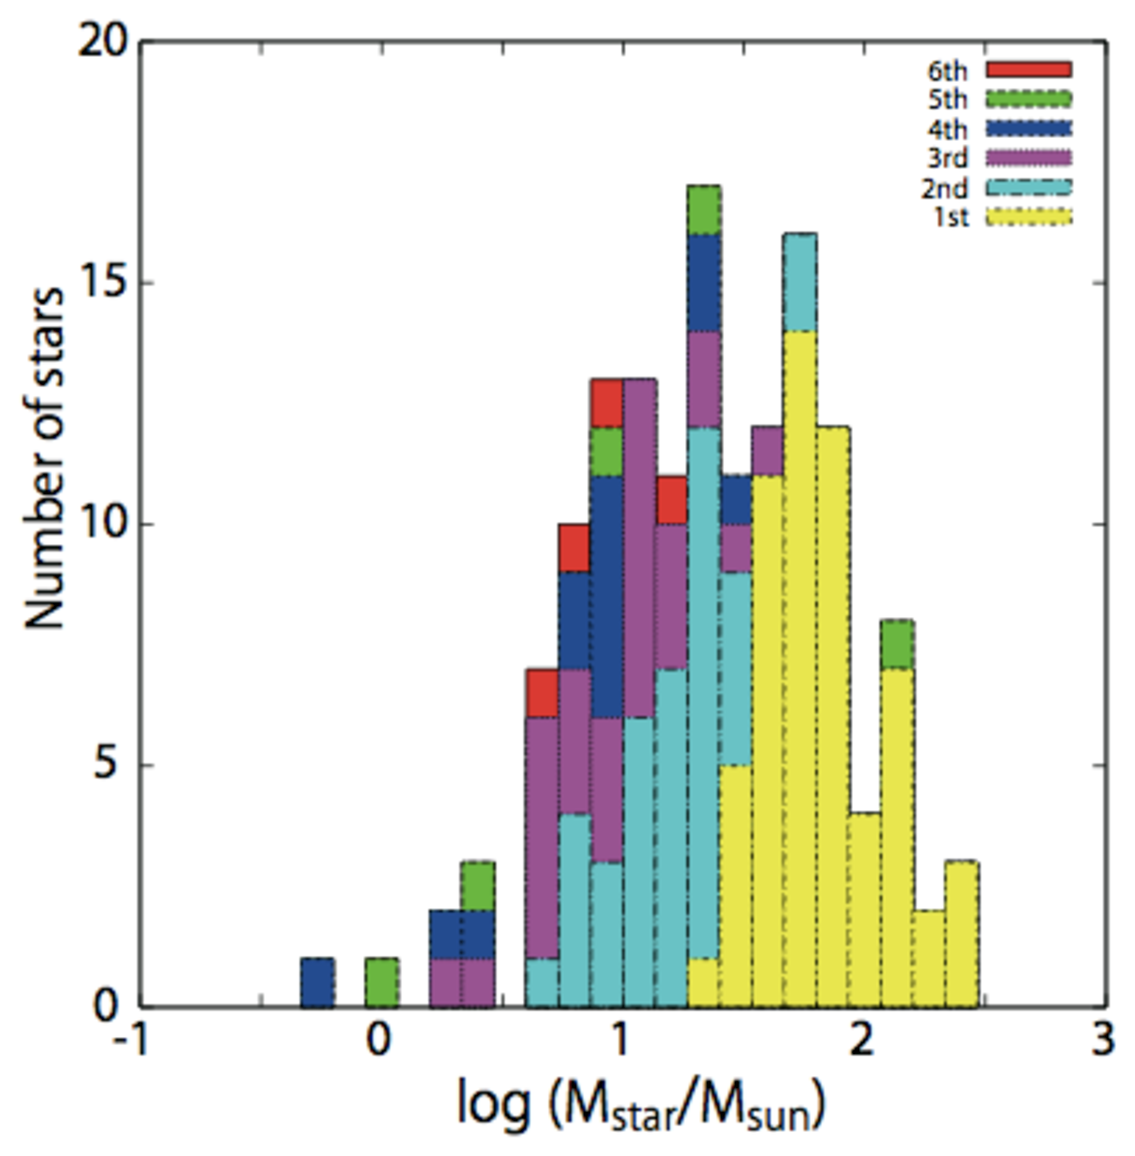
\includegraphics[width=8cm]{EoR/c03/c03.s2.f3.eps}}
	\caption{$B%7%_%e%l!<%7%g%s$K$h$C$FF@$i$l$?=iBe@1=i4|<ANL4X?t$N0l(B
 $BNc(B \citep{2014ApJ...792...32S}$B!#$3$N7W;;$G$O!"E57?E*$K$O(B$10-100M_\odot$$B!"3d9g$O>/$J$$$,(B$>100M_\odot$$B$d(B$<10M_\odot$$B$N=iBe@1$bB8:_!#$*$h$=(B1/3$B$,C1FH@1!"$=$l0J30$G$OJ#?t$N@17O$H$7$FCB@8!#(B}\label{KH3}
\end{figure}

\begin{figure}[!h]
	\centering\vspace*{1cm}
	{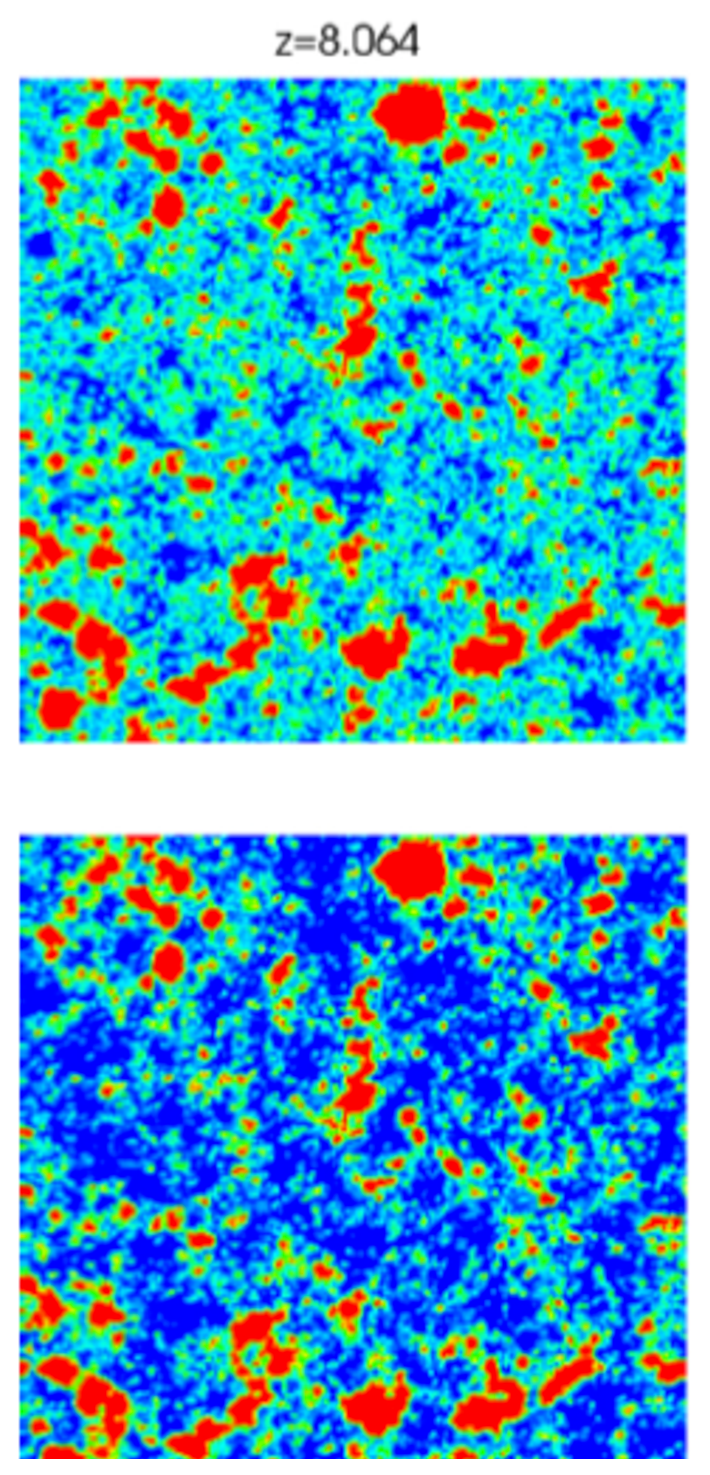
\includegraphics[width=5cm,angle=90]{EoR/c03/c03.s2.f4.eps}}
	\caption{$B%_%K%O%m!<$r9MN8$7$?>l9g(B($B:8?^(B)$B$H9MN8$7$J$$>l9g(B($B1&?^(B)$B$N(B
 $B@VJ}JP0\(B$z\approx8$$B$G$NEEN%9=B$(B($B@V$,EEN%NN0h!"@D$,Cf@-NN0h(B)$B!#%_%K%O%m!<(B
 $B$r9MN8$7$?>l9g!"ItJ,EEN%$5$l$?NN0h(B($BNP$NNN0h(B)$B$,@j$a$kBN@Q$,B?$/$J$j!"%H(B
 $B%`%=%s;6Mp$N8w3XE*8|$,A}2C$9$k(B \citep{2012ApJ...756L..16A}$B!#(B}\label{KH2} 
\end{figure}

EoR$B$N=i4|CJ3,$d(BCD$B$O!"=iBe@17A@.$K$h$C$F;O$^$k!#=iBe@1$O!"%_%K%O%m!<(B
($T_{\rm vir}<10^4$K, $B$b$7$/$O(B $10^4<M/M_\odot < 10^{7-8}$)$BFb$G@8$^$l$k$H?.$8$i(B
$B$l$F$$$k$,!"$3$N:]!"=iBe@1$N7A@.$O<g$K?eAGJ,;RNd5Q$K$h$C$F0z$-5/$3$5$l!"(B
$B8=:_$N@1(B($B<oB2(BI$B@1(B)$B$H$O0[$J$j=E85AG$r4^$^$J$$;v$+$i<oB2(BIII$B@1(B(Population
III star)$B$H$b8F$P$l$k(B\footnote{$B=E85AG$r4^$^$J$$@1$G$"$C$F$b!"@17A@.NN0h$,(B
$BEEN%!&2rN%mU<M$N1F6A$r<u$1$F$$$J$$>l9g$K$O<oB2(BIII.1$B@1!"$3$l$i$N1F6A$r<u$1(B
$B$?8e$K7A@.$5$l$k<!@$Be$N@1$O<oB2(BIII.2$B@1$H6hJL$9$k(B
\citep{2008AIPC..990.....O}$B!#$=$N0UL#$G!"<oB2(BIII$B@1$H=iBe@1$NDj5A$O87L)$K(B
$B$O0lCW$7$J$$!#(B}$B!#(B

\begin{figure}[!t]
	\centering
	{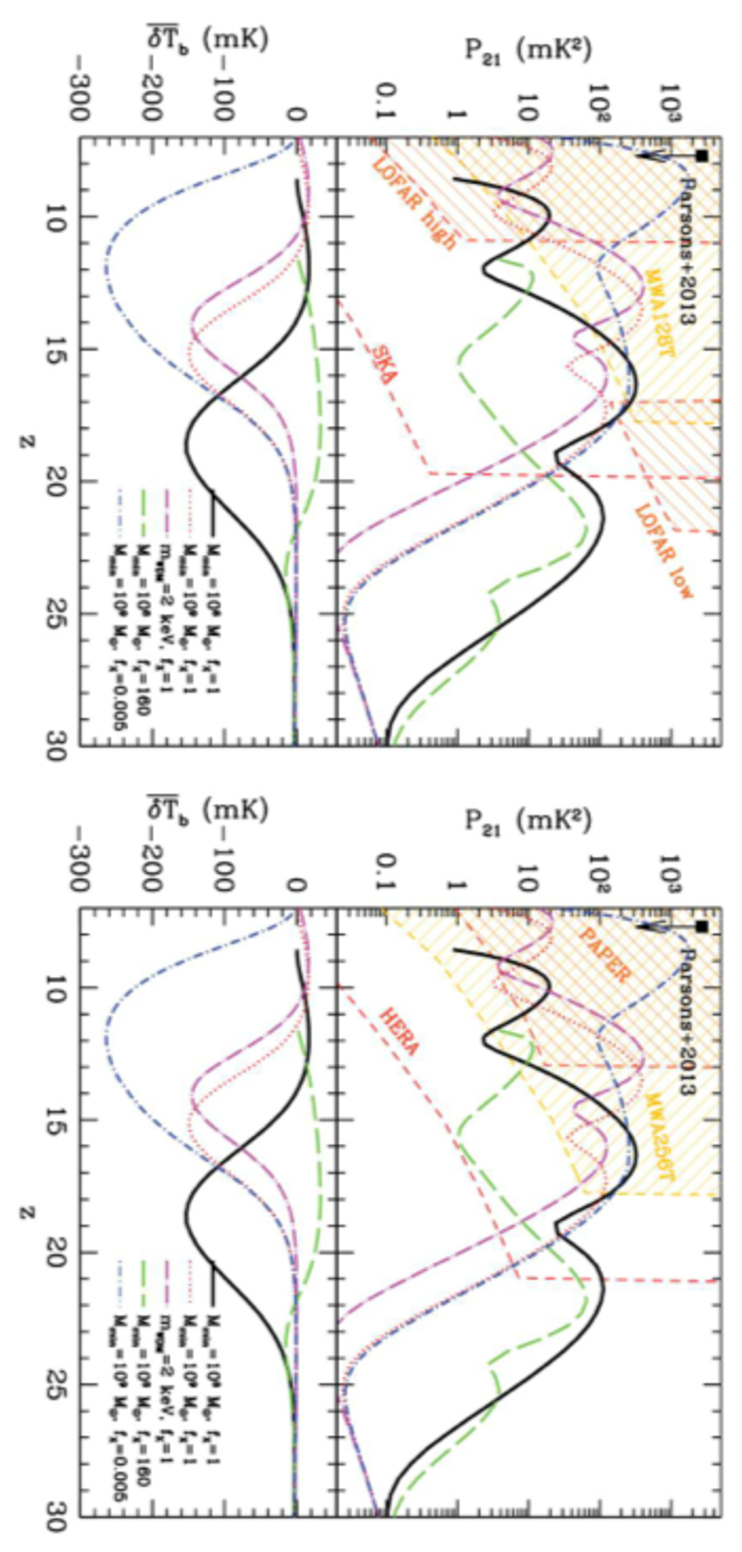
\includegraphics[width=5cm, angle=90]{EoR/c03/c03.s2.f5.eps}}
	\caption{$B>eCJ(B: $k=1/\rm Mpc$$B$K$*$1$k5eJ?6Q$7$?%Q%o!<%9%Z%/%H%k(B$P_{21}$$B$N?J2=(B $B!#$3$3$G!"(B$P_{21}$$B$O!"(B$P_{21}\equiv k^3/(2\pi^2V) \overline{\delta T_b}(z)^2\langle |\delta_{21}({\bf k},z)|^2 \rangle_k $$B!"(B$\delta_{21}({\bf x},z)=\delta T_b({\bf x},z)/\overline{\delta T_b}(z)-1$$B$GDj5A$5$l$k!#2<CJ(B: $BJ?6Q(B$\delta T_b$$B$N?J2=(B}\label{KH4}
\end{figure}
\begin{figure}[!h]
	\centering
	{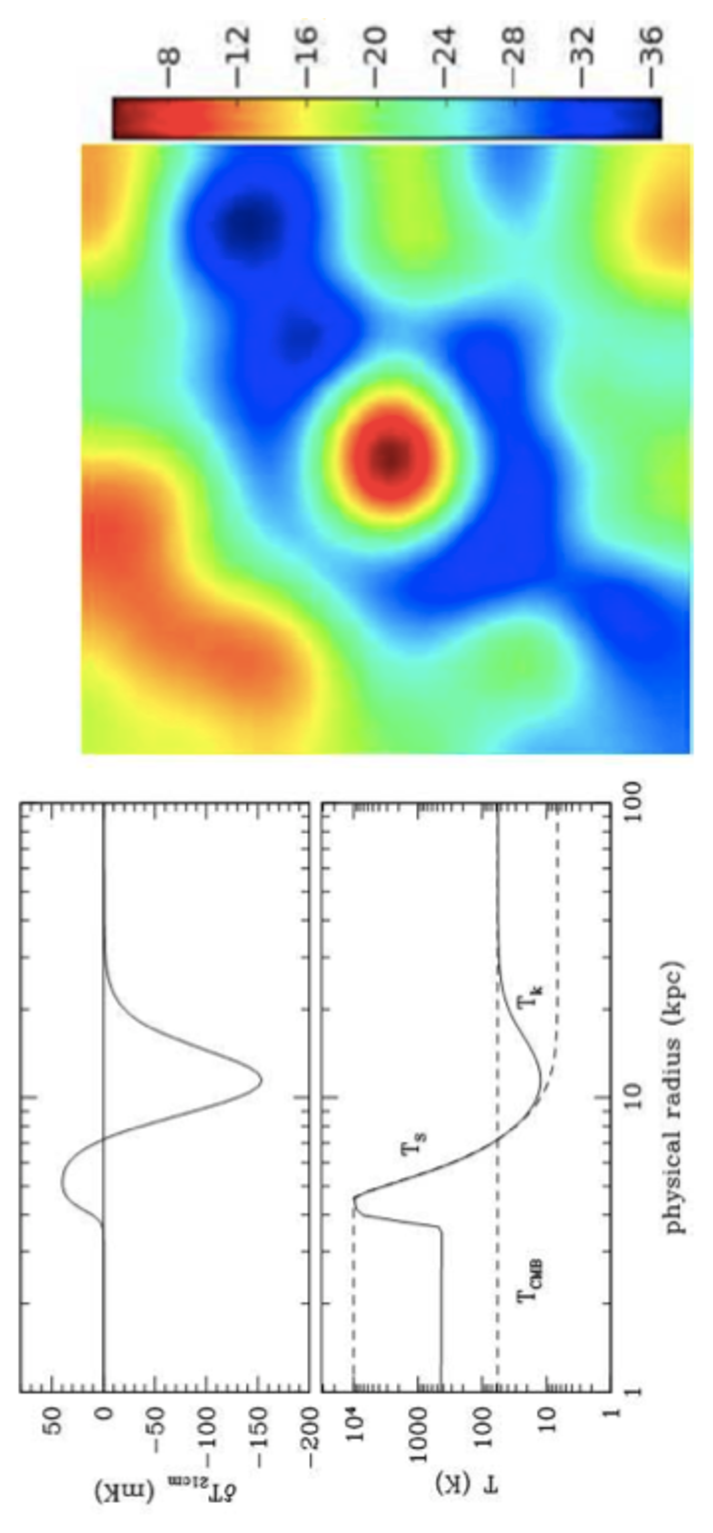
\includegraphics[width=5cm, angle=270]{EoR/c03/c03.s2.f6.eps}}
	\caption{$B:8?^(B: $BM}A[$J>u67$G$N<oB2(BIII$B@1(B + X$B@~8;$r4^$`6d2O<~$j$N%,(B
 $B%929EY(B($BGK@~(B)$B$H%9%T%s29EY(B($B<B@~(B)($B2<CJ(B)$B$H(B$\delta T_b$($B>eCJ(B) \citep{2008ApJ...684...18C}$B!#1&?^(B: $B$"$k$R$H$D$N1'ChO@E*L)EY%T!<%/(B $B$G7A@.$5$l$?L)=8$7$?6d2OFb$K<oB2(BIII$B@1(B + X$B@~O"@1(B + $B<oB2(BII$B@1$,B8:_$7$?>l9g$N(B$\delta T_b$$BJ,I[(B \citep{2014arXiv1405.2085A}$B!#(B $B%7%_%e%l!<%7%g%sNN0h%5%$%:$O!"0lJU(B40 comoving Mpc$B$G(B, $B%S!<%`I}(B $\Theta=2'$$BAjEv$NJ?3j2=$r9T$C$?8e$N?^$G$"$k!#?^Cf?4$NL)EY%T!<%/%5%$%:$O(B$\sim7$Mpc$\sim 10'$$B$KAjEv$9$k!#:8?^$G$O!"EEN%NN0h$9$030(B($BEEN%GHLL(B)$B$G2CG.$K$h$k51@~NN0h(B, $B$=$N$^$o$jNd$?$$%,%9$K$h$k5[<}NN0h$,8+$($k!#1&?^$G$O(B$\delta T_b>0$$B$N51@~NN0h$,8+$($J$$$,!"%S!<%`I}$r>.$5$/$7$?>l9g(B($B6u4VJ,2rG=$r>e$2$?>l9g(B)$B$K$O8+$($k2DG=@-$b$"$k!#(B}
	\label{KH5}
\end{figure}

2000$BG/:"$h$j?tCM%7%_%e%l!<%7%g%s$K$h$k=iBe@17A@.$N8&5f$,3hH/$K$J$j!"Bg<A(B
$BNL(B($\ge100M_\odot$)$B$N<oB2(BIII$B@1$,8IN)$7$F7A@.$5$l$k!"$$$o$f$k!H(Bone Pop III
star per one minihalo$B!I%Q%i%@%$%`$,?.$8$i$l$F$-$?(B(e.g.,
\cite{2002Sci...295...93A, 2002ApJ...564...23B, 2006ApJ...652....6Y}) $B!#(B
$B6aG/$G$O!"B??t$N%_%K%O%m!<%5%s%W%k$rMQ$$$?%7%_%e%l!<%7%g%s$K$h$C$FI}9-$$(B
$B<oB2(BIII$B@1<ANL$,<B8=$5$l$k;v$b<($5$l(B(e.g., \cite{2014ApJ...781...60H},
\cite{2014ApJ...792...32S})$B!"0l$D$N%_%K%O%m!<Fb$GJ#?t$NHf3SE*7Z$$(B
($10-100M_\odot$)$B@1$,@8$^$l$k2DG=@-$b;XE&$5$l$F$$$k(B(e.g.,
\cite{2009Sci...325..601T, 2010MNRAS.403...45S, 2011ApJ...737...75G,
2014ApJ...792...32S}, $B?^(B\ref{KH3})\footnote{$B6aG/$N798~$H$7$F$O%_%K%O%m!<(B
$BFb$N%,%9J,Nv$O5/$3$j$&$k$H$$$&8+J}$,B?$$!#$7$+$7!"$=$l$iJ,NvJR$,@1$K$J$k(B
$B$+!"$b$7$/$O$=$N$^$^Cf?4@1$K9_Ce$9$k$+$O$^$@5DO@$,<}B+$7$F$$$J$$!#(B}$B!#<oB2(B
III$B@1$N=i4|<ANL4X?t(B(Initial Mass Function: IMF) $B$O!"$3$l$i@1$+$i$NJ|<M$N(B
$B%9%Z%/%H%k%(%M%k%.!<J,I[(B(Spectral Energy Distribution: SED)$B$N9E$5(B
(hardness)$B$K4XO"$9$k!#$^$?!"(BX$B@~O"@1$,7A@.$5$l$k>l9g!"(BX$B@~$NBg$-$JJ?6Q<+M3(B
$B9TDx$K$h$j!";g30@~$GEEN%$5$l$k>l9g$HHf$Y$F$J$a$i$+$JEEN%9=B$$,$G$-$k$H9M(B
$B$($i$l$k(B \citep{2013MNRAS.431..621M}$B!#$3$N$h$&$K!"<oB2(BIII$B@1$N(BIMF$B$d7A@.N($O(B
$BEEN%9=B$$NH/C#$HL)@\$K4XO"$9$k!#(B



$B$7$?$,$C$F!"=iBe@17A@.!&?J2=$NM}O@$O(BCD, EoR$B$N%b%G%j%s%0$N:]$K=EMW$H$J$k!#(B
$B=iBe@17A@.$K$*$$$F!"<g$K$=$N7A@.$rAK32$9$k$N$O(BLyman-Werner$B%P%s%ImU<M$K$h(B
$B$k?eAGJ,;R$N8w2rN%$G$"$j(B(e.g., \cite{2000ApJ...534...11H})$B!"6aG/$G$O!"$3(B
$B$N?eAGJ,;R2rN%8w;R$NmU<MM"Aw$b9MN8$7$?BgNN0h(B($\ge 100$Mpc)$B:FEEN%%7%_%e%l!<(B
$B%7%g%s$b$J$5$l$F$$$k(B (\cite{2012ApJ...756L..16A} $B?^(B\ref{KH2})$B!#(B 



$B$^$?6aG/$G$O!"@2$l>e$,$j4|$K$*$1$k%P%j%*%s$H%@!<%/%^%?!<$NB.EY:9$N8z2L$b(B
$BE7BN7A@.2aDx$K1F6A$rM?$($k$H9M$($i$l$F$$$k(B \citep{2010PhRvD..82h3520T}$B!#(B
$B$3$N8z2L$r9MN8$7$?>l9g!"@17A@.2DG=$J%_%K%O%m!<<ANL$,Bg$-$/$J$j!"%O%m!<$N(B
$B7A@.;~4|$bCY$/$J$k;v$,?tCM%7%_%e%l!<%7%g%s$K$h$C$F<($5$l$F$$$k(B
 \citep{2011ApJ...730L...1S, 2011ApJ...736..147G}$B!#$^$?!"$3$NB.EY:9$N8z2L(B
$B$O!">W7bGH$h$C$FBg6IE*$J2CG.$r0z$-5/$3$9;v$G(B21 cm $B%Q%o!<%9%Z%/%H%k$K1F6A(B
$B$rM?$($k;v$b9M$($i$l$k(B \citep{2012ApJ...760....3M}$B!#(B

CD$B$H(BEoR$B$K$*$1$k(B21 cm$B%Q%o!<%9%Z%/%H%k2r@O$K4X$7$F!";0$D$NFCD'E*$J;~4|$,$"(B
$B$k!#(B(1) IGM$B$N29EY$,!"(BWouthysen-Field$B8z2L$K$h$C$F(BLyman-$\alpha$$BmU<M$H6/$/(B
$B%+%C%W%k$9$k!V(BLyman-$\alpha$-pumping epoch$B!W(B, (2) IGM$B$,(BX$B@~$K$h$C$F2CG.$5(B
$B$l!"=y!9$K(BCMB$B29EY$rD6$($k!V(BX-ray heating epoch$B!W!"(B(3) $BEEN%%P%V%k$,1'ChO@(B
$BE*%9%1!<%k$G7A@.$5$l$k!V(BEpoch of Reionization$B!W!#$=$l$>$l$N;~4|$G!"(B21 cm
$B51EY29EY(B ($\delta T_b\equiv{(T_{\rm
s}-T_{\gamma}(z))}(1-e^{-\tau_{21}})/(1+z))$)$B$N?6I}$d6u4VMI$i$.$OA}I}$5$l(B
$B$k(B (\cite{2014MNRAS.439.3262M}, $B?^(B\ref{KH4})$B!#(B 

$B:$Fq$G$O$"$k$,!"%H%b%0%i%U%#!<(B($B3F@VJ}JP0\$G$N;#A|(B)$B$O=iBe6d2O$[$I>.$5$JE7(B
$BBN$rJ,2r$G$-$k$+$b$7$l$J$$!#=iBe6d2O$NJ|<M%9%Z%/%H%k$O!"6d2OFb$N@1<ANL4X(B
$B?t$d(BX$B@~8;$NM-L5$J$I$K$h$C$F7hDj$5$l$k$,!"$3$NJ|<M%9%Z%/%H%k$N7A$O<~JU$N(B
$BEEN%9=B$!"(B21 cm$B%9%T%s29EYJ,I[$K1F6A$rM?$($k!#$b$7!"=iBe6d2O<~0O$N(B21 cm$B%7%0(B
$B%J%k$,8!=P$G$-$l$P=iBe6d2O$NFCD'$K@)8B$,IU$1$i$l$k$+$b$7$l$J$$(B(e.g.,
\cite{2008ApJ...684...18C, 2014arXiv1405.2085A})$B!#(B 
$BNc$($P!"Nd$?$$6d2O4V%,%9Fb$K;g30@~$H(BX$B@~$NJ|<M8;$,B8:_$9$k>l9g$r9M$($k(B($B?^(B
\ref{KH5}$B:8(B)$B!#J|<M8;IU6a$G$O!"2CG.$K$h$C$F%,%929EY$,(BCMB$B29EY$r>e2s$k$,!"EE(B
$BN%NN0hFb$G$OCf@-?eAG3d9g$,Hs>o$K>.$5$$0Y!"(B21 cm$B$N%7%0%J%k$O8+$($J$$(B
($\delta T_b\approx0$)$B!#$7$+$7!"$=$N30B&$NEEN%GHLL$KAjEv$9$kItJ,$G(B
$B$O!"Cf@-?eAG$,;D$C$F$*$j!"$+$D!"2CG.$K$h$C$F%,%929EY$,(BCMB$B29EY$r>e2s$k0Y!"(B
21 cm$B51@~(B($\delta T_b>0$)$BNN0h$,8=$l$k!#$h$j30B&$G$O!"Dc29%,%9$G$"$k(B
$B$?$a(B21 cm$B5[<}(B($\delta T_b<0$)$BNN0h$,8=$l$k$,!"$5$i$K30B&$G$O!"(BWF$B8z2L(B
$B$K$h$k%,%929EY$H%9%T%s29EY$N%+%C%W%j%s%0$,==J,$K5/$3$i$:!"(B21 cm$B%7%0%J%k$O(B
$B8+$($J$/$J$k!#0J>e$N$h$&$J?6$kIq$$$O!"J|<M%9%Z%/%H%k$N$+$?$A$K$h$C$F0c$$(B
$B$,@8$8$k!#Dj@-E*$K$OJ|<M%9%Z%/%H%k$r$h$j9E$/$9$k$[$I!"51@~NN0h$,9-$,$j5[(B
$B<}NN0h$,8+$($J$/$J$k798~$H$J$k!#(BAhn$B$i$O!"1'ChO@E*%7%_%e%l!<(B
$B%7%g%s$K$h$C$F$h$j8=<BE*$J>u672<$GL)=8$7$?6d2O<~0O$N(B$\delta T_b$$BJ,I[$rMM!9(B
$B$r7W;;$7!"6d2OJ|<M%9%Z%/%H%k$K$h$k(B21 cm$B%7%0%J%kJ,I[$N0c$$$r5DO@$7$F$$$k(B
(\cite{2014arXiv1405.2085A}, $B?^(B\ref{KH5}$B1&(B)$B!#(B 
%初代銀河、Lyman-$\alpha$とX線強度の揺らぎ、スピン温度
\subsection{SKA1-low$B$K$h$k:FEEN%4|$NEEN%NN0h$N;#A|(B}
\label{c03.s2.ss4}
\subsubsection{$BF3F~(B}
$B:FEEN%4|$K$*$1$k6d2O4VJ*<A$NEEN%9=B$$N;#A|$O!"(BSKA$B$NL\I8$N0l$D$G$"$k!#:FEE(B
$BN%4|$NEEN%NN0h$N9=B$$O!"L$$@$h$/2rL@$G$-$F$$$J$$6d2O7A@.$NJ*M}$KIR46$G$"(B
$B$k0Y!"EEN%9=B$$N%9%1!<%k$d?J2=$r;#A|$9$k;v$,$G$-$l$P!"MM!9$J6d2O7A@.%7%J(B
$B%j%*$N6hJL$d8w8;$NJ|<M%9%Z%/%H%k%?%$%W$N6hJL$,2DG=$H$J$k!#$3$3$G$O!"$=$N(B
$B0Y$N6qBNE*$J<jK!$r@bL@$9$k!#(B

SKA$B$N@h6nBN(B(precursor)$B$G$"$k(BMWA$B$d(BLOFAR$B$G$O46EY$,Dc$$$N0Y!"%Q%o!<%9%Z%/%H%k(B
$BEy$NE}7WE*4QB,$,%a%$%s$H$J$k!#0lJ}$G!"(BSKA1-low$B$G$O!"(Bi) 21 cm$B51@~$H6d2O$NAj(B
$B8_Aj4X(B(e.g., \cite{2007ApJ...660..1030F, 2007MNRAS.375..1034W}), ii) $BmU(B
$B<M6/EYMI$i$.$N3NN(J,I[(B(e.g., \cite{2009MNRAS.397..1138H,
2009MNRAS.397..1454B}), iii) $B8D!9$NEEN%NN0h(B, iv) $B%/%(!<%5!<$,;YG[E*$J(BHII
$BNN0h$J$I$N4QB,(B(e.g., \cite{2004Natur.432..194W, 2005ApJ...633..552K,
2006MNRAS.369L..66V})$B$,2DG=$K$J$k$H4|BT$5$l$k!#(B

21 cm signal$B$H6d2O$NAj8_Aj4X$+$i$O!"(B"outside-in"($BDcL)EYNN0h$,@h$KEEN%$9$k%7(B
$B%J%j%*(B)$B$H(B"inside-out"($B9bL)EYNN0h$,@h$KEEN%$9$k%7%J%j%*(B)$B:FEEN%$,6hJL$G$-$k!#(B
$BDL>o!"6d2O$rEEN%8w;R8;$H$7$?%7%_%e%l!<%7%g%s$G$O!"9bL)EYNN0h$,@h$KEEN%$9(B
$B$k!#$3$N>l9g!"6d2OJ,I[$H(B21 cm$B%7%0%J%k$O5UAj4X$r<($9$H4|BT$5$l$k!#(B


\subsubsection{$B=`?tCME*:FEEN%7W;;(B} 

$B=`?tCME*%b%G%k$N$R$H$D$G$"$k(BGALFORM$B$K!"4JN,2=$7$?<h$j07$$$G$NEEN%9=B$7W;;(B
$B$rAH$_9~$`(B(e.g., \cite{2013MNRAS.428..2467K})$B!#$3$N7W;;$G$O!"EEN%8w;R8;<~(B
$B$j$G$NEEN%8w;RJ|<MN($K1~$8$FEEN%NN0h$r7A@.$7!"6aK5EEN%NN0h$N%*!<%P!<%i%C(B
$B%W$O8w;R?t$NJ]B8$r9MN8$7$FL7=b$J$/07$o$l$k!#$^$?!"EEN%8w;R8;$H$7$FMM!9$J(B
$B6d2O%b%G%k$rAH$_9~$`$3$H$,2DG=$G$"$k!#(B

\subsubsection{$BEEN%NN0h$H6d2O7A@.(B}$B!!(B

$BD6?7@1GzH/$K5/0x$9$k%"%&%H%U%m!<$K$h$k@17A@.AK32$"$j$N>l9g(B($BD6?7@1GzH/%U%#!<(B
$B%I%P%C%/%b%G%k(B)$B$HL5$7$N>l9g$G$N!"=`?tCME*:FEEN%7W;;7k2L$NHf3S$r<($9!#D6?7@1GzH/%U%#!<%I%P%C%/%b%G%k(B
$B$G$O!"Dc<ANL6d2O7A@.$,AK32$5$l!"Bg<ANL6d2O$KJP$C$?8wEY4X?t$K$J$C$F$*$j!"(B
$B$=$l$>$l$N%b%G%k$G$N6d2O$N8wEY4X?t$O!"4QB,$r:F8=$9$k$h$&$K%b%G%k2=$5$l$F(B
$B$$$k(B($BL@$k$$ItJ,$7$+4QB,$HHf3S$G$-$J$$$N$G!"0E$$ItJ,$OG$0U@-$r;}$?$;$k;v$,(B
$B$G$-$k(B)$B!#$3$N7W;;$G$O!"3F;~4|$K$*$1$k6d2O4VJ*<A$NJ?6QCf@-?eAG3d9g$O8_$$$K(B
$BEy$7$/$J$k$h$&$KD4@0$5$l$F$$$k!#$9$J$o$A!"$U$?$D$N%b%G%k$N0c$$$O!"!V$"$k(B
$BJ?6QEEN%EY$rC#@.$7$?$H$-!"EEN%8w;R8;$H$7$F!">.<ANL6d2O$,;YG[E*$+Bg<ANL6d2O$,(B
$B;YG[E*$+!W$H$J$C$F$$$k!#$=$N7k2L!"J?6QCf@-?eAG3d9g$OF1$8$G$bEEN%NN0h$N%5(B
$B%$%:J,I[$OBg$-$/0[$J$k(B($B?^(B\ref{KH7})$B!#Dc<ANL6d2O$,;YG[E*$J>l9g!"B??t$N>.%9(B
$B%1!<%k(BH{\textsc{ii}}$BNN0h$,8=$l$k(B \citep{2013MNRAS.428..2467K}$B!#(B
\begin{figure}[!t]
	\centering
	{\includegraphics[width=10cm, angle=90]{EoR/c03/c03.s2.f7.eps}}
	\vspace{-1cm}
	\caption{GALFORM$B$rMQ$$$?(B500Mpc$B7W;;NN0h$N7W;;7k2L!#:8?^(B: $BD6?7@1Gz(B
 $BH/%U%#!<%I%P%C%/$r(B
	$B9MN8$7$?>l9g!"1&?^(B: $BD6?7@1GzH/%U%#!<%I%P%C%/$rL5;k$7$?>l9g!#(BKim et al. in prep.}\label{KH7}
\end{figure}

%\subsubsection{$B%/%(!<%5!<<~0O$NCf@-?eAG(B}$B!!(B%
%$B$$$/$D$+$N@VJ}JP0\(B$z\sim6$$B$N%/%(!<%5!<<~JU$G$O!"ItJ,E*$KCf@-$JEEN%NN0h$N(B
%$BB8:_$,<(:6$5$l$k!#:G6a$G$O!"(B$z\sim7$$B$N%/%(!<%5!<<~0O$G6d2O4VJ*<A5/8;$N(B
%Lyman-$\alpha$ damping wing$B$,8!=P$5$l!"Cf@-%,%9$,B8:_$r<($9$h$j6/$$>Z5r(B
%$B$H$J$C$?(B \citep{2011MNRAS.416L..70B}$B!#(B 
%14/12/6 $B>JN,(B($B!v:G6a$G$O!"(B$z\sim6$ QSOs$B$N%9%Z%/%H%k$K$b(BGP trough$B$,$_$D$+$j!"Cf@-?eAG$NB8:_$r<(:6(B, Becker et al. (2014)$B!#(BTotani et al. 2014$B$G$O!"(BGRB afterglow$B$N5[<}@~7O$N2r@O$+$i(B$z\sim5.8$$B$GCf@-?eAG$,;D$C$F$$$k;v$r<(:6!#(BSKA$B$G$3$N$h$&$J>l=j$r4QB,$G$-$l$P!"(B21 cm$B$N%7%0%J%k$,4|BT$G$-$k(B?)
%\\\\
%{\bf SKA1-low$B$N;#A|46EY(B}
% $B$3$N@a$O!"<($5$l$F$$$kCM$N;29MJ88%$bM?$($i$l$F$*$i$:!"?.Mj@-$,ITL@$J$N$G$6$C$/$j>JN,$7$^$9!#(B
%$B$3$3$G$O!"Ds0F$5$l$$$k(BSKA1-low$B$N%Y!<%9%i%$%s%G%6%$%s$N:FEEN%4|$NEEN%NN0h;#A|$KBP$9$k46EY$r8+@Q$b$k!#(BSKA1-low$B$O!"(B866$B$N%9%F!<%7%g%s$G9=@.$5$l!"$=$l$>$l(B45m$B$N%9%F!<%7%g%sFb$K(B256$B$N%"%s%F%J$,B8:_$9$k!#$3$3$N2r@O$G$O!"H>7B(B650$B%a!<%H%kFb$K0lMM$K%"%s%F%J$,CV$+$l$F$$$k$H2>Dj$9$k!#(B$\nu<200\rm MHz$$B$G$N%7%9%F%`29EY$O(B$T_{sys}\approx 250[(1+z)/7]^{2.6}$K$B$G$"$k!#$3$N(Bconfiguration$B$G$N3QEYJ,2rG=$O!"$3$N?6F0?t$G$*$h$=(B5.4 arcmin$B$G$"$j!"(Bprimary beam width$B$O(B$\theta_b=3.4$ degrees$B$H$J$k!#7k2L$H$7$F(Brms noise $B$O!"(B
%\begin{equation}
%\Delta T_b \approx 0.9 {\rm mK} \left(\frac{1+z}{8.5}\right)^{2.6}\left(\frac{\Delta \nu}{1{\rm MHz}}\frac{t_{int}}{1000{\rm hr}}\right)^{-1/2} \left(\frac{\theta_b}{6'}\right)^{-2}
%\end{equation}
%$B$H$J$k!#(B\\\\

\subsubsection{$B%7%_%e%l!<%7%g%s7k2L$N(BSKA1-low$B$K$h$kLO5<4QB,(B}
\begin{figure}[!t]
	\centering
	{\includegraphics[width=9cm, angle=90]{EoR/c03/c03.s2.f8.eps}}
	\vspace{-0.8cm}
	\caption{SKA1-low$B$G$N%7%_%e%l!<%7%g%s7k2L$NLO5<4QB,!#$3$3$G$O!"D6?7@1GzH/%U%#!<%I%P%C%/(B
	$B$,8z2LE*$KF/$$$?>l9g$N7k2L$r<($9!#(B
	$B:8>e?^!'%7%_%e%l!<%7%g%s7k2L!#(B
	$B1&>e?^!'A07JJ|<M$J$7$NLO5<4QB,!#(B
	$B:82<?^!'A07JJ|<M9~$_$G!"(BSKA-1 low$B$K$h$k(B1000$B;~4V4QB,$r2>Dj!#(B
	$B1&2<?^!'46EY$r(B1/2$B$K$7$?>l9g$NLO5<4QB,?^!#(B}\label{KH8}
\end{figure}
\begin{figure}[!h]
	\centering
	{\includegraphics[width=9cm, angle=90]{EoR/c03/c03.s2.f9.eps}}
	\vspace{-0.8cm}
	\caption{$B?^(B8$B$HF1MM$@$,!"D6?7@1GzH/%U%#!<%I%P%C%/$rL5;k$7$?>l9g$N7W;;7k2L$NLO5<4QB,(B}
	\label{KH9}
\end{figure}
$BD6?7@1GzH/%U%#!<%I%P%C%/$r9MN8$7$?7W;;NN0h(B$(1 {\rm Gpc}/h)^3$$B$N%7%_%e%l!<(B
$B%7%g%s$N7k2L$r(BSKA1-low$B$GLO5<4QB,$r$9$k(B($B;29MJ88%$OL$Ej9F(B)$B!#A07JJ|<M$H$J$k(B
$B6d2O7OFb%7%s%/%m%H%m%sJ|<M$d7O306d2O$NJ|<M$O:FEEN%4|$N(B21 cm$B%7%0%J%k8!=P$NBg(B
$B$-$J>c32$H$J$k!#$3$3$G$O!"J,2r2DG=E7BN$N$+$i$NJ|<M$OA4$F<h$j=|$1$?$H2>Dj(B
$B$9$k!#?^(B\ref{KH8}$B$O!"(BSKA1-low$B$G(B1000$B;~4V4QB,$r2>Dj$7!"A07JJ|<M=|5n(B
 \citep{2008MNRAS.390..1496G, 2011MNRAS.418..516G}$B8e$NLO5<4QB,%^%C%W$G$"(B
$B$k!#7k2L!"D6?7@1GzH/%U%#!<%I%P%C%/$,8z2LE*$G$"$k>l9g$K@8@.$5$l$kEEN%NN0h(B
$B$N;#A|$O2DG=$G$"$m$&!#(B 

$B0lJ}$G!"D6?7@1GzH/%U%#!<%I%P%C%/$J$7$N%b%G%k$N>l9g!":G$bBg$-$JEEN%NN0h$O(B
$B4QB,$G$-$=$&$@$,!"<B:]$K$O%N%$%:$HA07JJ|<M=|5n$K$h$C$FEEN%NN0h$N%3%s%H%i(B
$B%9%H$,2<$2$i$l$k$?$a!"(BSKA1-low$B$G$N;#A|$O:$Fq$G$"$m$&(B($B?^(B\ref{KH9})$B!#(BSKA2
$B$G$O(B4$BG\DxEY46EY$,NI$$0Y!";#A|$G$-$k2DG=@-$,$"$k!#(B



% \subsubsection{$B:FEEN%4|$NEEN%GHLL$N4v2?3XE*8|$_(B}
% $B%/%(!<%5!<$O!"@17A@.6d2O$KHf$Y$F9E$$J|<M%9%Z%/%H%k;}$D$?$a!"4v2?3XE*$K8|(B
% $B$$EEN%GHLL$r;}$D!#EEN%GHLL$G$O!"29EY$,9b$/ItJ,EEN%$7$??eAG$,;D$C$F$$$k$?(B
% $B$a!"(B$\delta T_b>0$$B$H$J$j!"$h$j30B&$G$ONd$?$$6d2O4V%,%9$K$h$j(B$\delta
% T_b<0$$B$H$J$k!#$3$l$K$h$j!"EEN%GHLL$N8|$5$rJ,2r$G$-$k$[$I==J,$J6u4VJ,2rG=(B
% $B$,$"$l$P!"EEN%GHLLIU6a$N(B21 cm$B%7%0%J%k$rD4$Y$k;v$G$I$N$h$&$JE7BN$,8w8;$G$"(B
% $B$k$+6hJL$9$k;v$,$G$-$k!#(B

%{\bf SKA1-low$B$N;kLn(B}
%$B%7%_%e%l!<%7%g%s$O!":FEEN%$N8e4|CJ3,$K$*$$$F(B100Mpc($\sim$1$BEY(B)$B0J>e$N6u4V%9%1!<%k$NCf@-NN0h$NB8:_$rM=8@$9$k!#(B\\\\

\subsubsection{$B$^$H$a(B} 

$B6d2O%b%G%k$N0c$$$K$h$C$F4|BT$5$l$kEEN%9=B$$,Bg$-$/0[$J$k$?$a!"$b$7(B21 cm$B%7(B
$B%0%J%k$N6u4VJ,I[$r4QB,$G$-$l$P!"Nc$($PD6?7@1GzH/$K$h$k%U%#!<%I%P%C%/$,8z(B
$B2LE*$KF/$$$F$$$k$+$I$&$+$J$I$N6d2O7A@.$NJ*M}$rM}2r$9$k;v$,$G$-$k!#(B
SKA1-low$B$N>l9g!"6/$$D6?7@1GzH/%U%#!<%I%P%C%/$,8z2LE*$KF/$$$F$$$l$P$G$NEE(B
$BN%NN0h$OJ,2r$G$-$k!#$7$+$7!"D6?7@1GzH/$N%U%#!<%I%P%C%/$,8z2LE*$G$J$/!"Dc(B
$B<ANL6d2O$K$h$kEEN%8w;R6!5k$,;YG[E*$G$"$k>l9g!"$h$j9b$$6u4VJ,2rG=$,I,MW$H(B
$B$J$k!#EEN%NN0h$rJ,2r$G$-$k9b$$J,2rG=$K2C$($F!":G$bBg$-$JEEN%9=B$(B($B$3$N7W;;(B
$B$G$O(B$100$Mpc$B$G$*$h$=(B1$BEY$N3QEY$KAjEv(B)$B$N;#A|$r$9$k0Y$K$O!"(BSKA1-low$B$N;kLn$O>/(B
$B$J$/$H$b?tEY$OI,MW$G$"$k!#(B
%SKA1-lowによる再電離期の電離領域の撮像
\subsection{$B;#A|4QB,(B}
\label{c03.s2.ss5}

$B:FEEN%4|$N4QB,$G$O(B 21 cm$B@~$N51EY29EY$,F@$i$l$k!#(B21cm$B@~$N51EY29EY$r2r@O$7$F!"(B
$B:FEEN%4|$NJ*M}$d=i4|E7BN$K$D$$$F$N>pJs$rF@$k;v$,$G$-$k!#2r@O$N<jK!$H$7$F!"(B
$BE}7WE*<jK!$H;#A|$,$"$k!#E}7WE*<jK!$H$7$FBeI=E*$J$b$N$O%Q%o!<%9%Z%/%H%k$K(B
$B$h$k2r@O$G$"$k!#(B21 cm$B@~$N51EY29EY$N;}$DMI$i$.$N>pJs$rE}7WE*$K=hM}$7!":FEE(B
$BN%4|$G$NJ*M}$K@)8B$r2C$($k!#0lJ}!";#A|$OE}7WE*$J=hM}$G$O$J$/!"F@$i$l$?(B
21cm$B@~$N%7%0%J%k$+$iA|$r9g@.$7!":FEEN%4|$NMM;R$rD>@\8+$h$&$H$9$k$b$N$G$"(B
$B$k!#$3$N@a$G$O;#A|$K$h$C$F:FEEN%4|$N2?$,J,$+$k$H9M$($i$l$F$$$k$+$^$H$a$k!#(B 

$B;#A|$r9T$&$K$O!"EEGH43>D7W$,==J,$J3QEYJ,2rG=$r$b$DI,MW$,$"$k!#$7$+$7!"4Q(B
$BB,$GJ,2rG=$r>e$2$k$H$$$&;v$O4QB,$KH<$&%N%$%:$N4sM?$r6/$/<u$1$k;v$K$J$k!#(B
$B%N%$%:$KBP$7$FM%0L$K%7%0%J%k$,F@$i$l$?$+$I$&$+$O!"(BS/N$B$r;H$C$FH=Dj$9$k!#(B
S/N$B$O4QB,CM$H4QB,8m:9$NHf$G$"$k!#;#A|$r9T$&$?$a$K$O$3$N(BS/N$B$,==J,$KBg$-$$(B
$BI,MW$,$"$k(B(1$B0J>e(B)$B!#%"%s%F%J$NM-8z3+8}LL@Q(B$ A_{eff}$$B$H%7%9%F%`29EY(B$
T_{sys}$$B$r8GDj$9$k$H!"(BS/N$B$O4QB,;~4V$d4QB,<~GH?t$N%A%c%s%M%kI}!"$=$7$F4Q(B
$BB,$NJ,2rG=$K0MB8$9$k!#?^(B\ref{yoshiura.fig:1}$B$O(BSKA$B$K$h$C$F;#A|$,$I$l$/$i(B
$B$$$NJ,2rG=$G2DG=$+$r<($7$?$b$N$G$"$k(B \citep{2013ExA....36..235M}$B!#(B21 cm$B@~(B
$B$N%7%0%J%k$,(B 1 mK$BDxEY$G$"$k$H$7$F(B($B<B:]:FEEN%4|$G$N51EY29EY$NBg$-$5$O(B 1mK
$BDxEY$H9M$($i$l$F$$$k(B)$B!"K>1s6@$K5a$a$i$l$k(B$ A_{eff}/T_{sys}$$B$r<($9$b$N$,(B
$B3%?'$NNN0h$G$"$k!#<P@~$G0O$^$l$?NN0h$O!"(BSKA($BCf?4$N%3%"$,H>7B(B2Km)$B$N<B8=2D(B
$BG=$J(B$ A_{eff}/T_{sys}$$B$G$"$j!"Cf$K$"$k(B3$BK\$N<B@~$O>e$+$iJ*M}E*3+8}LL@Q$,(B
$0.25~\rm km^2$,$1~\rm km^2$,$2.5~\rm km^2$$B$N>l9g$G$"$k!#$3$N<B@~$h$j2<$K!"(B
$B3%?'$NNN0h$,$"$l$P$=$NJ,2rG=$G$N;#A|$,2DG=$G$"$k$HM=A[$5$l$k!#(B 

\begin{figure}[t]
 \centering
 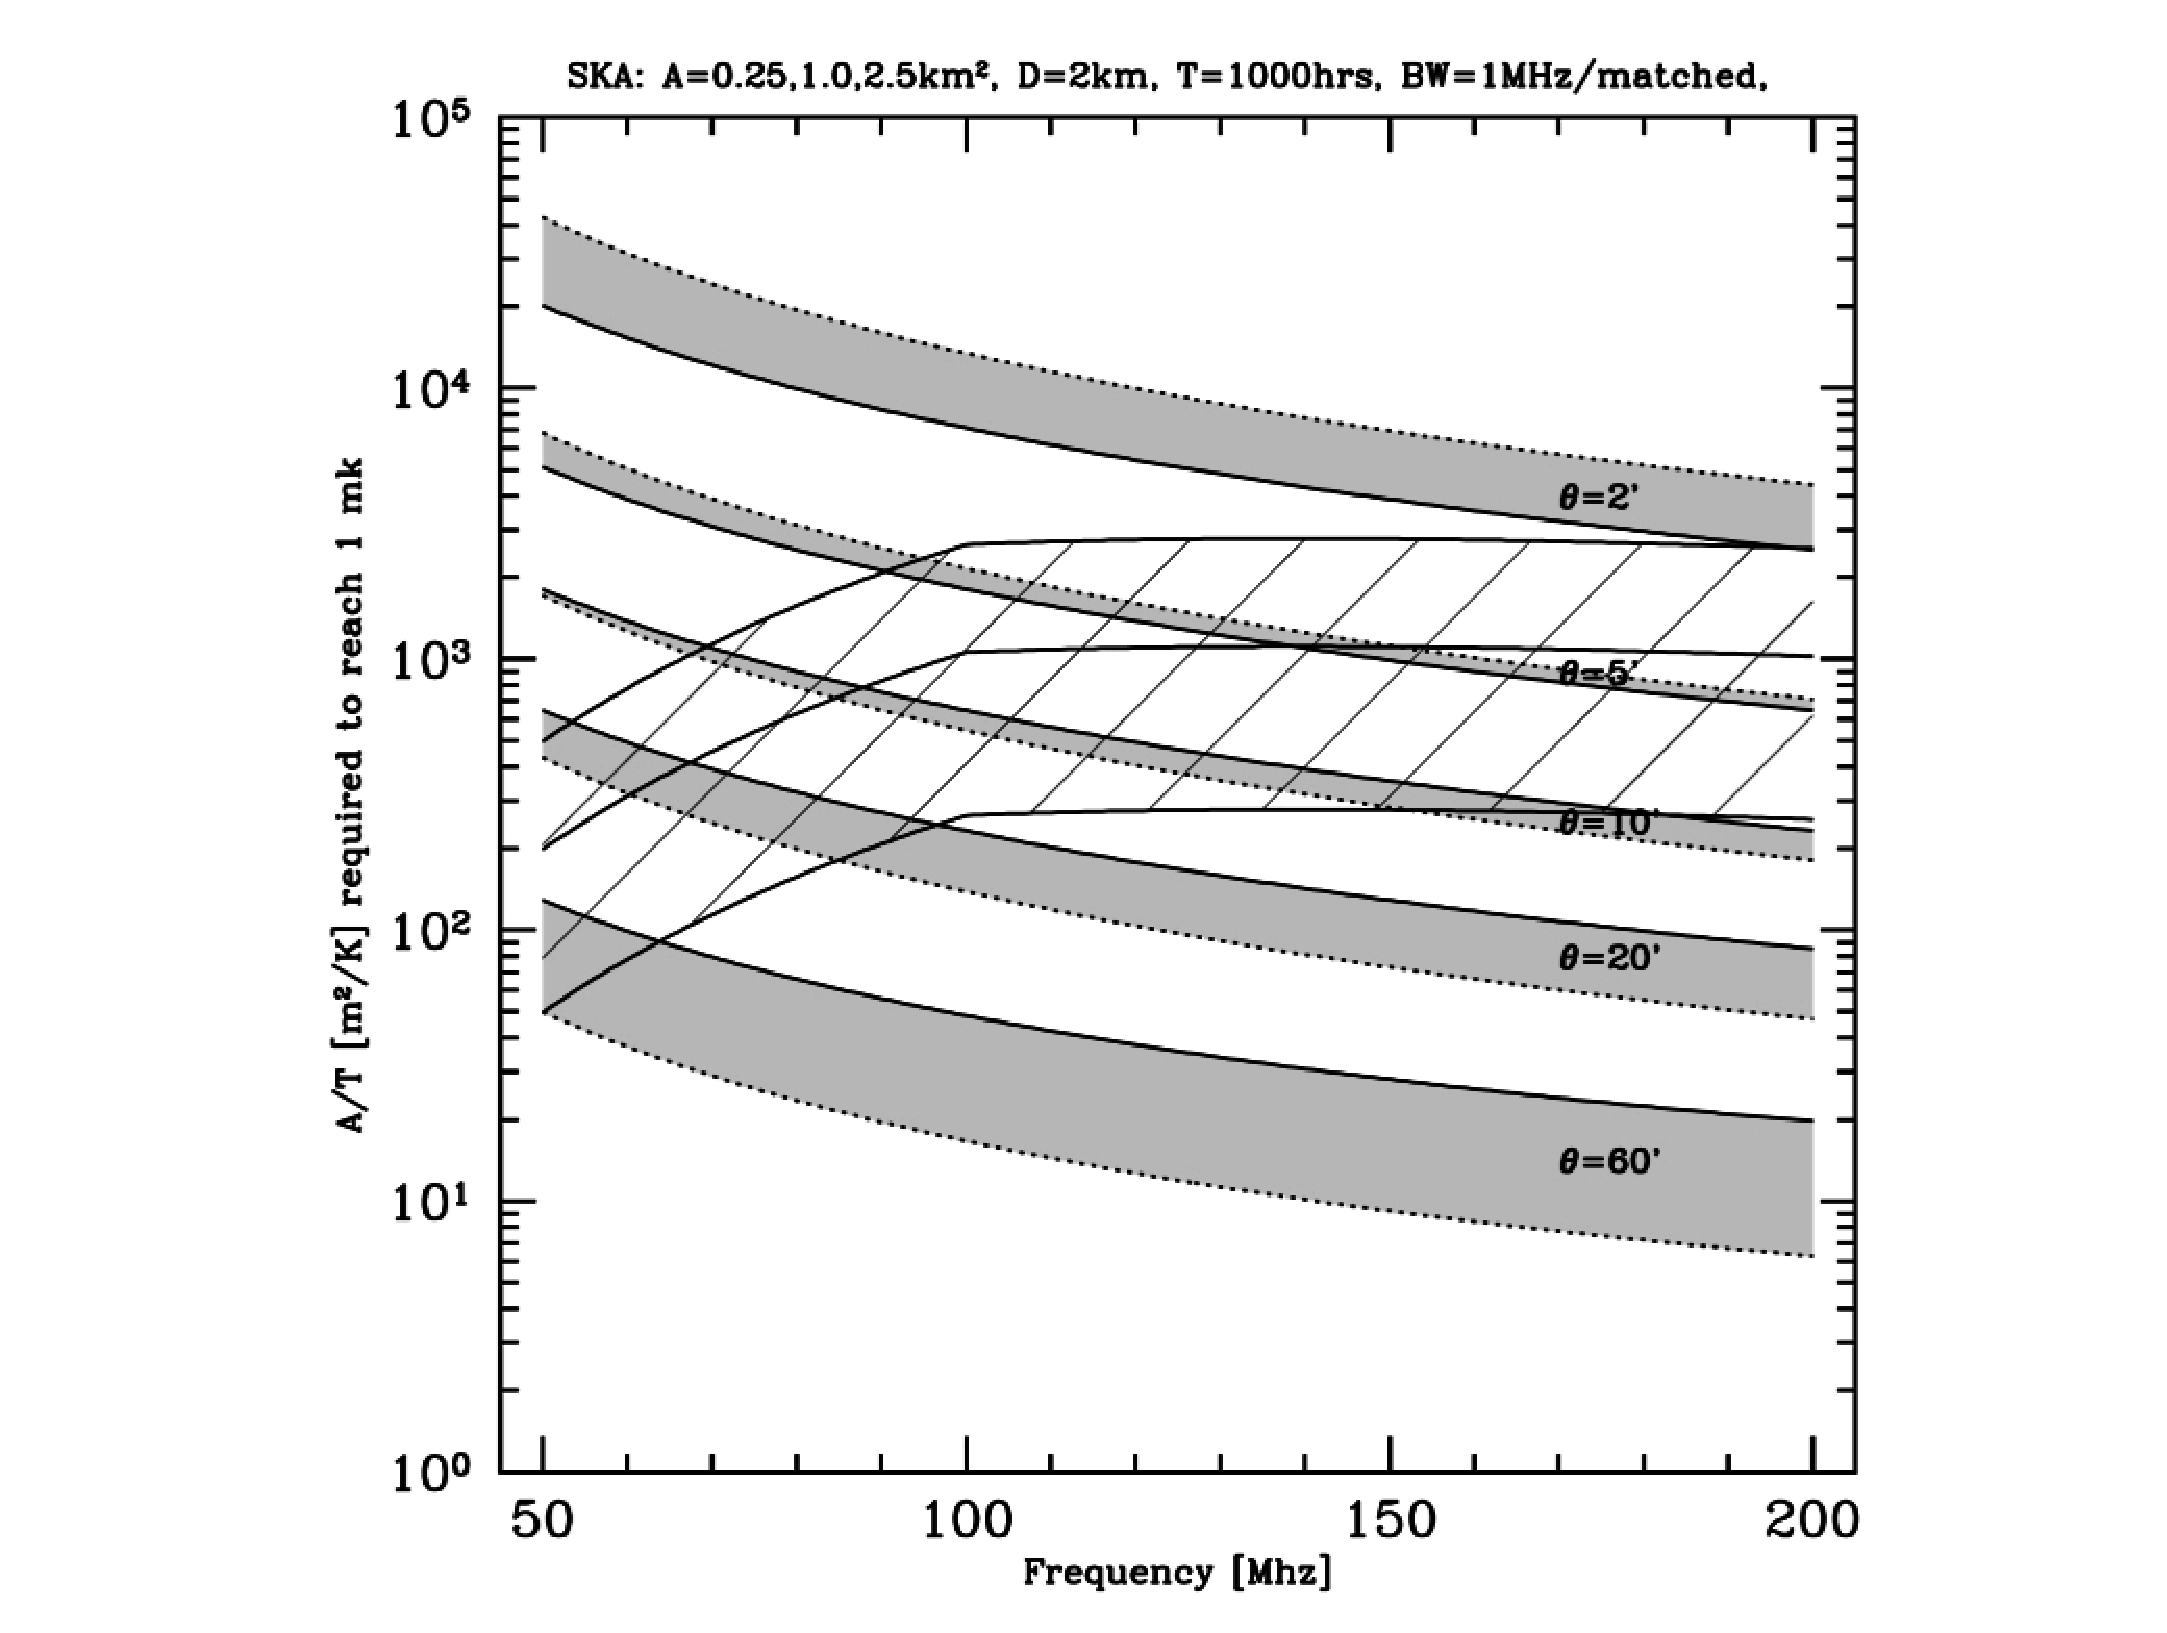
\includegraphics[width=10cm,clip]{EoR/c03/c03.s2.f10.eps}
 \label{yoshiura.fig:1}
\caption{1mK$B$N51EY29EY$+$i;#A|$9$k$?$a$K5a(B
 $B$a$i$l$k(B$A_{eff}/T_{sys}$$B$r<($7$F$$$k!#=D<4$,(B$ A_{eff}/T_{sys}$$B$NBg$-$5!"(B
 $B2#<4$,<~GH?t$G$"$k!#3%?'$N@~$,J,2rG=$4$H$K5a$a$i$l$k(B$ A_{eff}/T_{sys}$$B$NBg$-$5!"<P@~$O(BSKA$B$G<B8=2DG=$J(B$ A_{eff}/T_{sys}$$B$NBg$-$5$rI=$9!#<P@~$h$j2<$K2+?'$$@~$,$"$l$P(BSKA$B$G$N;#A|$,2DG=$G$"$k!#(B}
\end{figure}


\subsubsection{$B;#A|$K$h$k2r@O(B}
$B;#A|$K$h$C$F:FEEN%4|$G$N(B21cm$B@~$N%^%C%W$rF@$F!"<!$KLdBj$J$N$O$=$l$r$I$N$h$&$K2r@O$9$k$+!"$H$$$&;v$G$"$k!#$3$3$G$O8=:_9M$($i$l$F$$$k2r@O<jK!$r>R2p$9$k!#(B\\

(a)$B%$%*%s2=%P%V%k(B : $B;#A|$rMQ$$$?2r@O$G$O%$%*%s2=%P%V%k$N%5%$%:J,I[$dFC0[E7BN<~$j$NNN0h$r07$&!#(B
$B%$%*%s2=%P%V%k$H$OCf@-?eAG$,%$%*%s2=$5$l$?NN0h$N$3$H$G!";#A|$r9T$C$F%$%*(B
$B%s2=%P%V%k$N7A$dJ,I[$r8+$k;v$G$=$NFCD'$rB*$($k;v$,$G$-$k!#$?$@$7!"%$%*%s(B
$B2=8w;R$rJ|<M$9$kE7BN$O1'Ch$K8IN)$7$FB8:_$7$F$$$kLu$G$O$J$/!"O"$J$j$r;}$C(B
$B$F$$$k!#$=$N$?$a%$%*%s2=NN0h$OJ#;($K=E$J$C$F$*$j2r@O$OMF0W$G$O$J$$!#2r@O(B
$B<jK!$H$7$F(Bspherical average method $B!"(B $B%$%*%s2=N($N%Q%o!<%9%Z%/%H%k!"(B
Friend of Freiend$B$N#3$D$NJ}K!$,9M$($i$l$F$$$k(B
 \citep{2011MNRAS.413.1353F}$B!#(B 

(b)$BFCJL$JE7BN(B : $B%/%'!<%5!<$d6d2OCD$N<~0O$G$O!"6/$$%$%*%s2=$d2CG.$N8z2L$r(B
$B<u$1$F51EY29EY$OFCD'E*$JJ,I[$r;}$D$H9M$($i$l$F$$$k!#;#A|$r9T$&;v$K$h$C$F!"(B
$B$=$l$i$N<~$j$NFCD'E*$JNN0h$,$_$D$+$l$P$=$N%5%$%:$d7A$+$i9b@VJ}JP0\$G$NE7(B
$BBN$N?6$kIq$$$rFCD'$E$1$k;v$,$G$-$k(B \citep{2012MNRAS.424..762D}$B!#(B 

(c)$B%H%]%m%8!<(B : $B;#A|$+$i%$%*%s2=NN0h$NJ,I[$rMxMQ$7$?!"%H%]%m%8%+%kB,Dj$H(B
$B$$$&$b$N$,9M$($i$l$F$$$k!#(B 
$B:FEEN%4|Cf$N%$%*%s2=NN0h$NFCD'$r$H$i$($k!#%_%s%3%U%9%-!<HF4X?t(B($B%$%*%s2=(B
$B%P%V%k$NBN@Q!"I=LL@Q!"J?6Q6JN(!"%*%$%i!<?t(B$\chi$$B$rF@$i$l$?NN0h$NCf$G7W;;(B
$B$7J?6Q$7$?$b$N(B)$B$r>pJs$H$7$F07$&!#$^$?!"%$%*%s2=NN0h$NFCD'$O%8!<%J%9(B$ 
g=1-\chi$$B$H$7$FI=8=$5$l$k!#8IN)$7$?NN0h$N?t$r(B$\rm N_{part}$$B!"$=$l$i$NNN(B
$B0hCf$N%H%s%M%k$N?t$r(B$N_{tunnel}$$B!"7j$N?t$r(B$ N_{cavity}$$B$H$9$k$H(B$\chi$$B$O(B
$B<!$N$h$&$K=q$1$k(B \citep{2006MNRAS.370.1329G,2011MNRAS.413.1353F}$B!#(B 
\begin{eqnarray}
 \chi=N_{part}-N_{tunnel}+N_{cavity}
\end{eqnarray}
$B0J>e$N$h$&$JJ}K!$G%$%*%s2=NN0h$rFCD'$E$1$k;v$K$h$C$F!":FEEN%$N%b%G%k$N@)(B
$B8B$K7R$,$k$H9M$($i$l$F$$$k!#$?$@$7!"%$%*%s2=%P%V%k$N;~$HF1MM$G(B21 cm$B@~$N%7(B
$B%0%J%k$NCf$+$i$I$N$h$&$K$7$F%$%*%s2=NN0h$N>pJs$@$1$r<h$j=P$9$+$,LdBj$K$J(B
$B$k!#(B 

\subsubsection{$B;#A|$K$h$k%5%$%(%s%9(B}
$B0J2<$G$O2r@O$N7k2L!":FEEN%4|$NJ*M}$K$D$$$F$I$N$h$&$J;v$,J,$+$k$H4|BT$5$l$F$$$k$+>R2p$9$k!#(B

(1)$B%$%*%s2=NN0h$NKDBg$J%G!<%?$+$i!"%/%'!<%5!<$N<wL?$d8wEY!"(BIGM$BCf$NCf@-EY(B
$B$K@)8B$,2C$($i$l$k(B \citep{2005ApJ...634..715W}$B!#%/%'!<%5!<$N<~0O$N%$%*%s(B
$B2=NN0h$,$?$@KDD%$9$k$@$1$J$i$P$=$N7A$O8w1_?m8z2L$K$h$C$FMq7A$H$J$k!#4QB,(B
$B$K$h$C$F<B:]$N7A$,J,$+$l$P%/%'!<%5!<$N%$%*%s2=8w;R$N<B:]$N8wEY$,J,$+$k(B
 \citep{2008MNRAS.386.1683G}$B!#7h$^$C$?J}8~$K$7$+J|<M$r9T$o$J$$>l9g!"$=$N(B
$B%$%*%s2=NN0h$O5e>u$G$J$/$J$k!#$=$3$+$i%/%'!<%5!<$N;}$D0[J}@-$,J,$+$j!";#(B
$BA|$G$-$?>l9g!"3hF06d2O3K$NJ|<M$N$b$D0[J}@-$K$D$$$F=i$N%^%C%T%s%0$H$J$k!#(B
$B$^$?!":FEEN%4|$h$jA0$N(BCD$B$K%/%'!<%5!<$,B8:_$7$F$$$?>l9g!"(BX$B@~$K$h$k2CG.$K(B
$B$h$C$F5[<}$,5/$3$kNN0h$HJ|<M$,5/$3$kNN0h$G(B21 cm$B@~$N51EY29EY$K(B$200$ mK$B$[$I$N(B
$B0c$$$,@8$8$k!#$3$l$[$I$N0c$$$,$"$l$P(BCD$B$N$h$&$J9b@VJ}JP0\1'Ch$b;#A|$G$-$k(B
 \citep{2010ApJ...723L..17A}$B!#(B 


(2)$B2D;k8wNN0h$G4QB,$5$l$?6d2OCD<~0O$N%$%*%s2=NN0h$N%5%$%:$d7A$,J,$+$l$P!"(B
$B%$%*%s2=8w;R$NJ|<M$N<($96d2O$NJ,I[$H$=$NJ,I[$N(Bbrightest member$B$N4X78$r?d(B
$BDj$G$-$k!#$=$3$+$i$^$@4QB,$5$l$F$$$J$$6d2OJ,I[$N8wEY4X?t$KBP$7$F@)8B$r2C(B
$B$($k;v$,$G$-$l$P!":FEEN%$,5/$-$k$?$a$K$O8=:_8+$D$+$C$F$$$k6d2O$N?t$G$OB-(B
$B$j$J$$$H$$$&LdBj$N2r7h$K7R$,$k$+$b$7$l$J$$!#(B 


(3)$B%Q%o!<%9%Z%/%H%k$O:FEEN%4|$N%Q%i%a!<%?$K46EY$,$"$k$,!"$=$l$i$N%Q%i%a!<(B
$B%?$O=LB`$7$F$$$F@)8B$,Fq$7$$!#%$%*%s2=NN0h$N7A$d%5%$%:$N>pJs$+$i!"$=$N=L(B
$BB`$r2r$/;v$,$G$-$k$H4|BT$5$l$F$$$k!#(B 


(4)$B:FEEN%4|$h$j0JA0$N(BCD$B$G$O!"%,%9$,2CG.$5$l$k;v$G51EY29EY$NBg$-$5$K(B100mK
$BDxEY$N0c$$$,@8$8$k!#$3$N>l9g!"?t==(BmK$B$N%N%$%:$G$b;#A|$9$k;v$,2DG=$H$J$k!#(B
$B51EY29EY$NJ,I[$O1'Ch$N=i4|$N@1$+$i$NJ|<M$HL)@\$K4X$o$C$F$$$k$N$G!"$3$N;~(B
$BBe$N;#A|$O=iBe@1$NFCD'$r<($9=EMW$J>Z5r$K$J$k$@$m$&!#(B 

%Regimes for Imaging
\subsection{21cm forest}
\label{c03.s2.ss6}

21cm$B@~$rMQ$$$?:FEEN%4|C5::$N0l$D$H$7$F!"%H%b%0%i%U%#!<$d%Q%o!<%9%Z%/%H%k(B
$B$H$OJL$N%"%W%m!<%A$G$"$k(B``21cm forest''$B$,$"$k(B
 \citep{2002ApJ...579....1F, 2006MNRAS.370.1867F}$B!#$3$l$O!"9b@VJ}(B
$BJP0\$NEEGHE7BN$+$i$N%9%Z%/%H%k$,!"6d2O4V%,%9!J(BIGM$B!K$dE7BN$K$h$C$F5[<}$r(B
$B<u$1!"5[<}@~$H$7$F4QB,$5$l$k$3$H$rMQ$$$k!#$9$J$o$A!"9bL)EY$NCf@-?eAG$,B8(B
$B:_$9$k>l=j$G$O!"EEGH8;$+$i$N85!9$N%U%i%C%/%9$OCf@-?eAG$K$h$k5[<}@~$H$7$F(B
$B4QB,$5$l!"5[<}@~$N?<$5$+$iCf@-?eAG$NL)EY$d!"%,%9$N29EY>uBV$rD4$Y$k;v$,$G(B
$B$-$k$N$G$"$k!#(B 
$B5[<}$NEY9g$$$rI=$9J*M}NL$G$"$k8w3XE*8|$_$O<0(B(\ref{eq:optical})$B$GI=$5$l$k!#(B
% $n_{{\rm H}}$$B$O?eAG$N?tL)EY!"(B$\delta$$B$O%,%9$ND62aL)EY!"(B$x_{{\rm HI}}$$B$O(B
% $BJ?6QCf@-?eAGN(!"(B$T_{{\rm S}}$$B$O%9%T%s29EY$rI=$9!#$^$?!"(B
% $A_{21}=2.85\times 10^{-15}s^{-1}$$B$O%"%$%s%7%e%?%$%s(BA$B78?t!"(B$H$$B$O%O%C%V%k(B
% $B%Q%i%a!<%?!"(B$dv_{||}/dr_{||}$$B$O%,%9$N;k@~J}8~$NB.EY8{G[$G$"$k!#(B 
% \begin{eqnarray}
% \tau_{21cm}(z)&=&\frac{3}{32\pi}\frac{h_{p}c^{3}A_{21cm}}{k_{{\rm B}}\nu_{0}^{2}}\frac{n_{{\rm H}}}{T_{{\rm S}}(1+z)dv_{||}/dr_{||}} \notag\\
% &=&9.6\times 10^{-3}x_{{\rm HI}}(1+\delta)\left(\frac{1+z}{10} \right)^{3/2}\left(1-\frac{T_{{\rm CMB}}}{T_{{\rm S}}}\right)\left[\frac{H(z)/(1+z)}{dv_{||}/dr_{||}}\right]
% \label{eq:optical}
% \end{eqnarray}
$BEEGHE7BN<+?H$N;}$D%9%Z%/%H%k$r(B$S_{{\rm in}}$$B$H$9$k$H!"5[<}$r<u$1$?8e$N%9(B
$B%Z%/%H%k(B$S_{{\rm abs}}$$B$O(B$S_{{\rm abs}}=(1-e^{-\tau_{21cm}})S_{{\rm
in}}$$B$HI=$5$l$k!#(B 


\paragraph{$B4QB,$5$l$k%9%Z%/%H%k(B}
$B<B:]$K4QB,$5$l$k%9%Z%/%H%k$K$O!"4QB,5!4o$N%N%$%:$,>h$C$F$/$k!#4QB,$5$l$k(B
$B%S%8%S%j%F%#$O(B 
\begin{equation}
V_{v}({\bold u})=\sum_{i}^{N_{sources}}I_{\nu}({\bold s})e^{-2\pi i {\bold u}\cdot{\bold s}}+n_{s}
\label{eq:visibility}
\end{equation}
$B$G$"$k!#(B${\bold u}=(u,v,w)$$B$O$"$k;~9o$G$N4p@~$N:BI8$rI=$7!"(B$I_{\nu}$$B$O4Q(B
$BB,$9$kEEGH8;$N6/EY!"(B${\bold s}=(l,m,n)$$B$O4QB,J}8~$HEEGH8;$NJ}8~$NM>89$r(B
$BI=$7$F$$$k!#$^$?!"(B$n_{s}$$B$OIU2CE*$J%N%$%:$G$"$j!"(B 
\begin{equation}
n_{s}=\frac{1}{\eta_{s}}\frac{SEFD}{\sqrt{N(N-1)t_{int}\Delta\nu}}
\label{eq:noise}
\end{equation}
$B$HI=$5$l$k!#(B$\eta_{s}$$B$O%7%9%F%`8zN((B, $\Delta \nu$$B$O(B,$B%P%s%II}(B $t_{int}$
$B$O@QJ,;~4V$G(BN$B$O%9%F!<%7%g%s$N?t$G$"$k!#$^$?!"(BSEFD$B$O(B{\rm sys}tem
equivalent flux density$B$G!"(B 
\begin{equation}
{\rm SEFD}=\frac{2k_{{\rm B}}T_{{\rm sys}}}{N_{{\rm dip}}\eta_{\alpha}A_{\rm eff}}
\label{eq:noise2}
\end{equation}
$B$G$"$k!#$3$3$G!"(B$T_{{\rm sys}}$$B$O%7%9%F%`29EY$H8F$P$l!"EE;R5!4o$N%N%$%:!\6u$+$i(B
$B$N%N%$%:!"(B$N_{{\rm dip}}$$B$O#1$D$N%9%F!<%7%g%s$"$?$j$N%@%$%]!<%k%"(B
$B%s%F%J$N?t$G!"(B$\eta_{\alpha}$$B$O%@%$%]!<%k8zN((B, $A_{\rm eff}$$B$O#1$D$N%@%$(B
$B%]!<%k%"%s%F%J$"$?$j$N<B8zLL@Q$rI=$7$F$$$k!#(B 


\paragraph{$B%7%_%e%l!<%7%g%s7k2L(B}
$B?^(B\ref{fig:forest1}, \ref{fig:forest2}, \ref{fig:forest3}$B$K(B21cm forest$B$N(B
$B%7%_%e%l!<%7%g%s7k2L$r<($9!#$3$l$i$N?^$O(B$z$=10,7.6,14$B$N>l9g$G$N(BLOFAR$B!"(B
SKA$B$rA[Dj$7$?>l9g$N(B21cm$B5[<}@~$rEEGH8;$N%U%i%C%/%9JL$GHf3S$7$F$$$k!#$3$l(B
$B$i$N7k2L$h$j8@$($k$3$H$H$7$F!":#2sA[Dj$7$?@VJ}JP0\$N>l9g$G$O!"(BLOFAR$B$G$O(B
$B6/$$5[<}@~$r4QB,$9$k;v$,$G$-$k$H$$$&$3$H$G$"$k!#$^$?!"(BSKA1$B$N%9%Z%C%/$@$H(B
$B%N%$%:$N1F6A$,>.$5$/!"%N%$%:$b4^$s$@<B:]$K4QB,$5$l$k%U%i%C%/%9(B$S_{{\rm
obs}}$$B$O!"(B$S_{{\rm obs}}\sim S_{{\rm abs}}$$B$G4QB,$9$k;v$,=PMh$k!#$^$?!"(B
$BCf@-?eAG$,$h$jB?$/;D$C$F$$$k9b@VJ}JP0\$[$I!"5[<}$O6/$/8=$l$k!#(B 
\begin{figure}[htbp]
   \centering 
   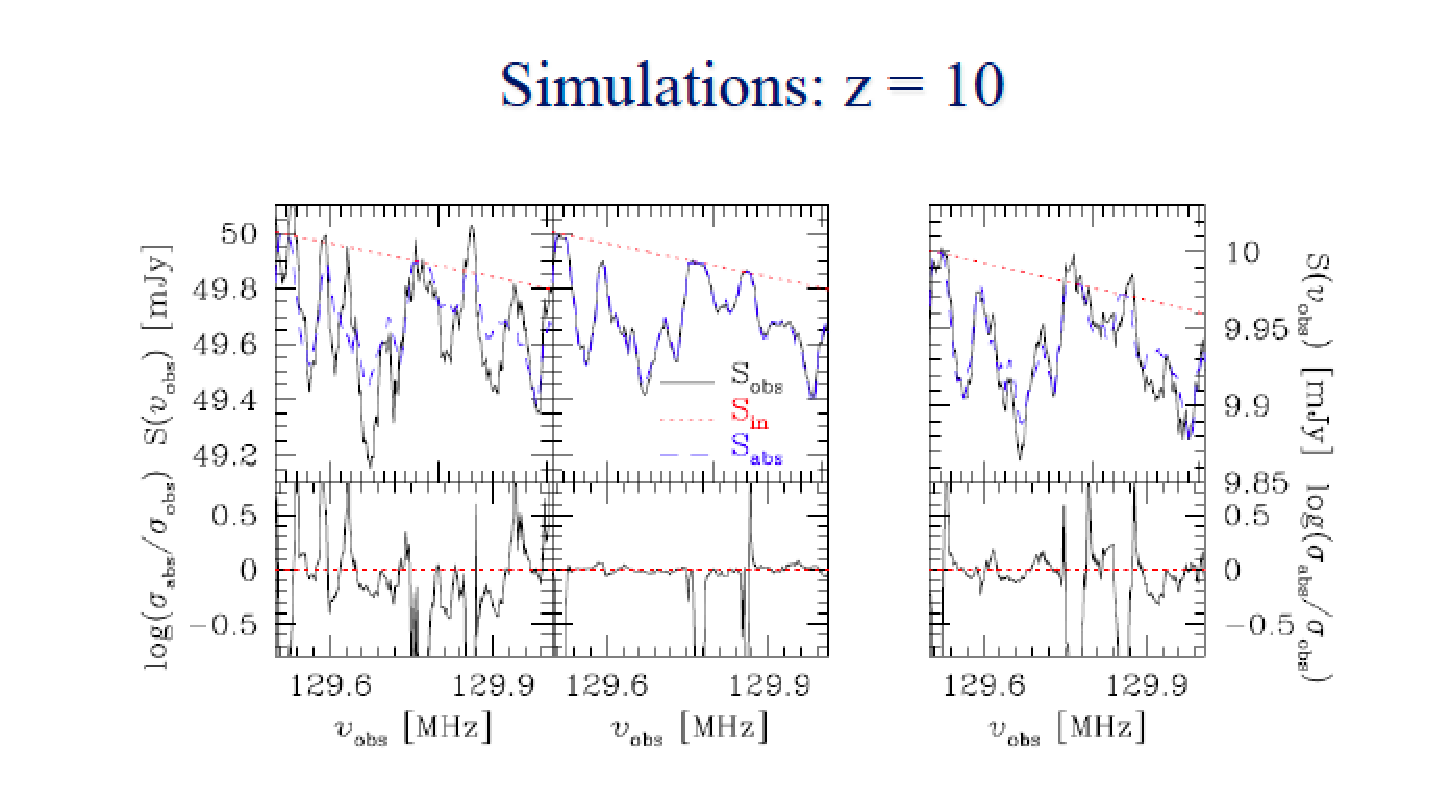
\includegraphics[scale=0.7]{EoR/c03/c03.s2.f11.eps}
   \caption{$z$=10$B$G$N7k2L!#(B$S_{{\rm in}}$$B$OEEGH8;K\Mh$N%9%Z%/%H%k$rI=$7$F$*$j!"(B$S_{{\rm abs}}$$B$O(B21cm$B5[<}@~$N%7%_%e%l!<%7%g%s7k2L$r!"(B$S_{{\rm obs}}$$B$O4QB,$K$h$k%N%$%:$b>h$;$?(B21cm$B5[<}@~$N7k2L$rI=$7$F$$$k!#$^$?!"(B$\sigma_{i}=S_{i}-S_{{\rm in}}$$B$G$"$k!#:8Fs$D$N%Q%M%k$OEEGH8;$N%U%i%C%/%9$,(B50mJy$B$N>l9g$G$N(BLOFAR$B$rA[Dj$7$?%N%$%:!J:8!K!"(BSKA1$B$rA[Dj$7$?%N%$%:!J1&!K$G$"$k!#$^$?!"1&$N%Q%M%k$O(BSKA1$B$rA[Dj$7$?$H$-$G%U%i%C%/%9$,(B10mJy$B$N>l9g$N7k2L$G$"$k!#(B$\Delta \nu=10{\rm kHz}$}
\label{fig:forest1}
\end{figure}
\begin{figure}[htbp]
   \centering 
   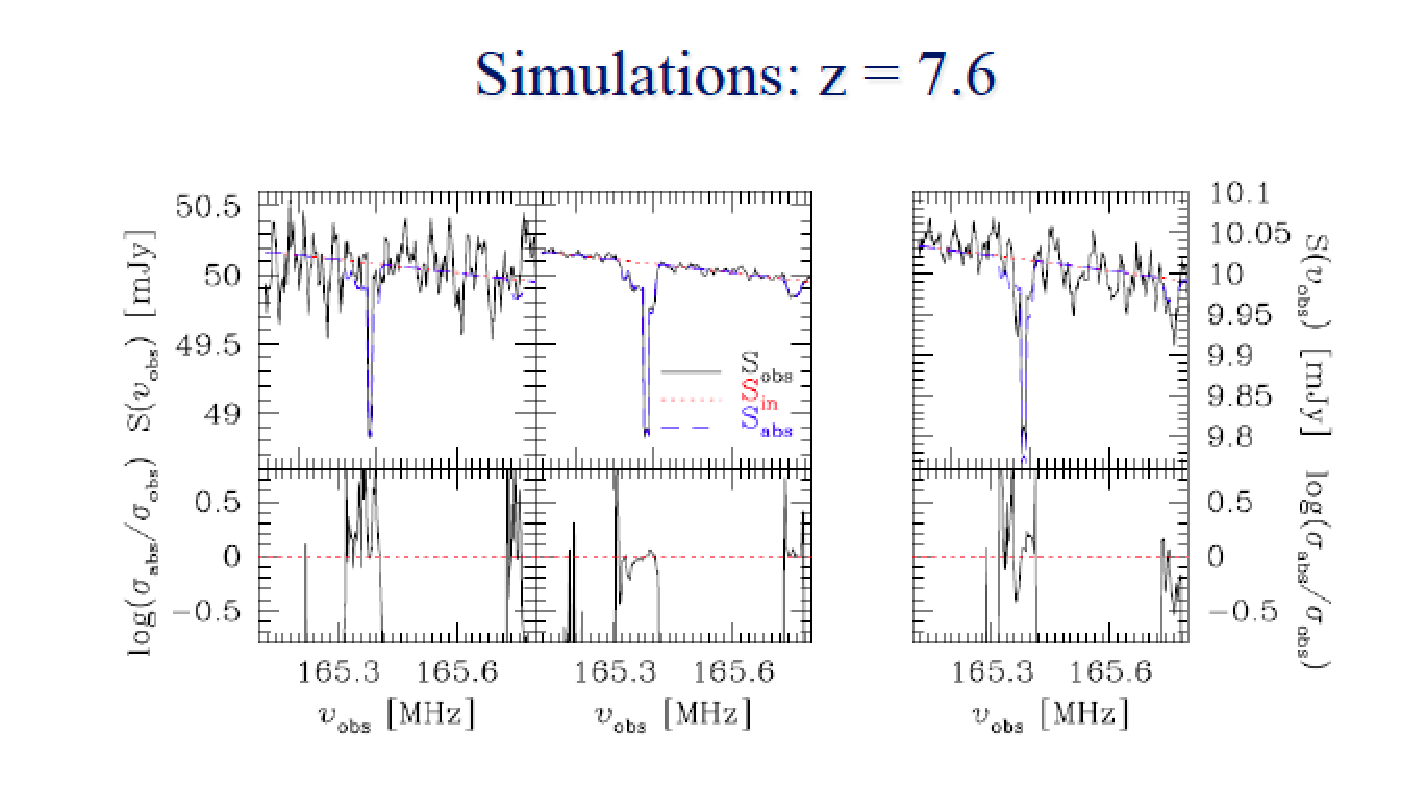
\includegraphics[scale=0.7]{EoR/c03/c03.s2.f12.eps}
   \caption{$z$=7.6$B$G$N%7%_%e%l!<%7%g%s7k2L!#@~$N@bL@$O!"?^(B\ref{fig:forest1}$B$N>l9g$HF1$8!#(B$\Delta \nu=5{\rm kHz}$}
\label{fig:forest2}
\end{figure}

\begin{figure}[htbp]
   \centering 
   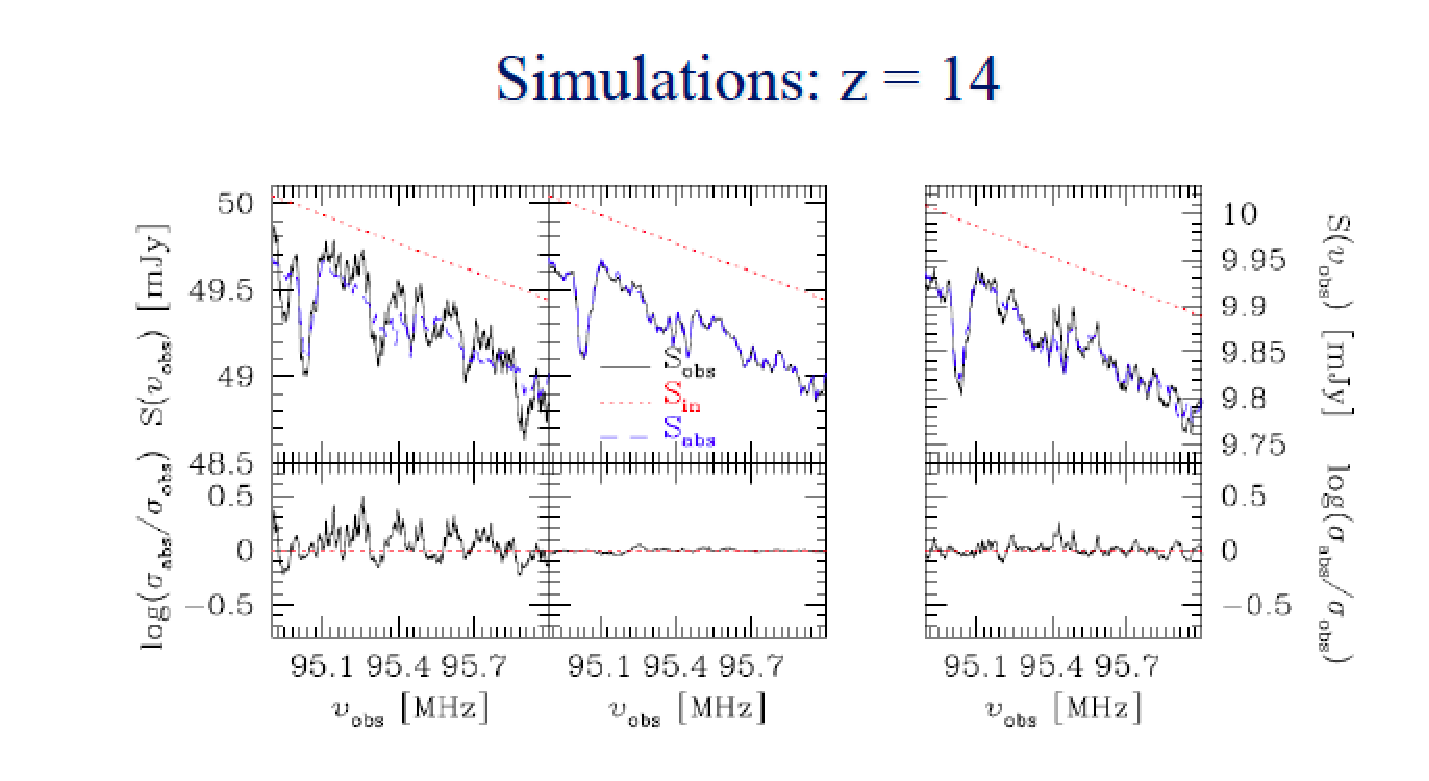
\includegraphics[scale=0.7]{EoR/c03/c03.s2.f13.eps}
   \caption{$z$=14$B$G$N%7%_%e%l!<%7%g%s7k2L!#@~$N@bL@$O!"?^(B\ref{fig:forest1}$B$N>l9g$HF1$8!#(B$\Delta \nu=20{\rm kHz}$}
\label{fig:forest3}
\end{figure}

\paragraph{$BMWLs$*$h$S5DO@(B}
\begin{itemize}
 \item $BGX7JE7BN8w$N5[<}@~$KCmL\$7$?(B21cm forest$B$O%H%b%0%i%U%#!<$d%Q%o!<%9%Z%/(B
$B%H%i%`$HAjJdE*$K:FEEN%4|$N$K$*$1$k6d2O4V%,%9$N29EY>uBV$J$I$N@-<A$rC5$k;v(B
$B$,=PMh$k!#(B
\item $B8=:_$N%7%_%e%l!<%7%g%s7k2L$@$H!"(BLOFAR$B$K$h$k4QB,$G$b5[<}@~$r8+$k;v$O2D(B
$BG=!#$?$@$7!"(B$\sim {\rm kHz}$$B$N?6F0?tJ,2rG=$,I,MW!#(B
\item $B6d2O4V%,%9$K$h$k5[<}$h$j$b!"%3%i%W%9$7$?E7BN$K$h$k5[<}$NJ}$,6/$$5[<}$r(B
$B0z$-5/$3$9!#(B
\item $B$=$b$=$bGX7JE7BN$,9b@VJ}JP0\$GB8:_$7$F$$$k;v$,I,MW>r7o$G$"$j!"8=:_!"(B
$z\sim 4$$B$G4QB,$5$l$F$$$kEEGH8;$N?tL)EY$r$h$j9b@VJ}JP0\$K30A^$7$FM=A[$5(B
$B$l$kA4E7$G$NEEGH8;$N?t$O(B$8\times 10^{2}-3\times 10^{4}$$B8DDxEY!J?^(B
\ref{fig:forest4}$B!K(B
 \citep{2002ApJ...577...22C,2009ApJ...704.1396X}$B!#(B 
\end{itemize}
\begin{figure}[htbp]
   \centering 
   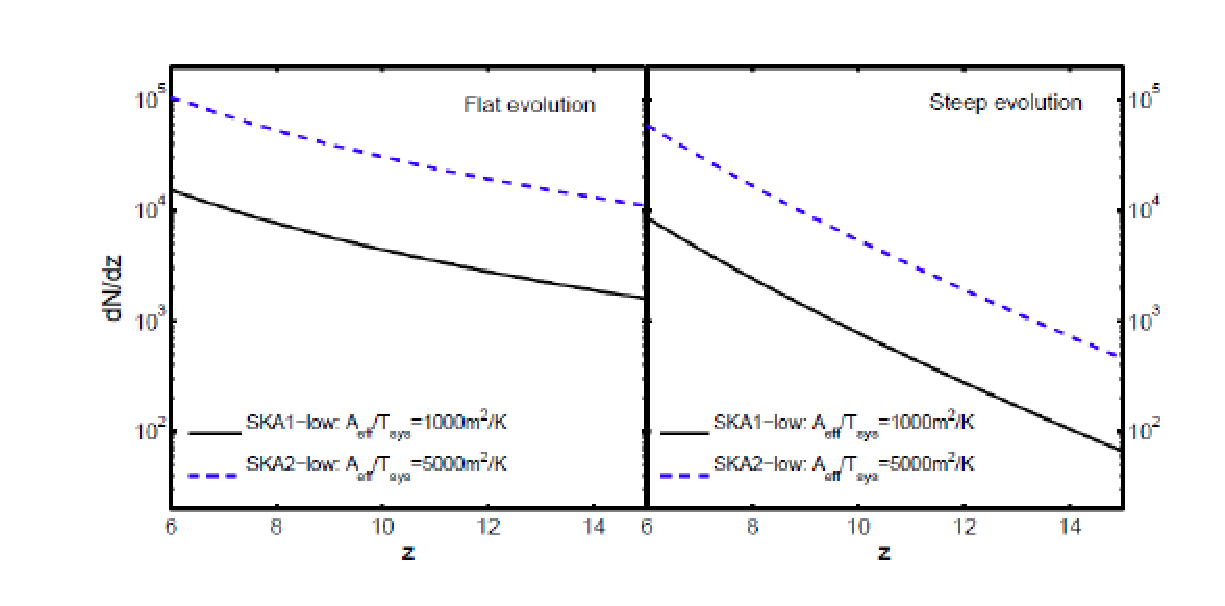
\includegraphics[scale=0.7]{EoR/c03/c03.s2.f14.eps}
   \caption{SKA1-low$B!J9u@~!K$H(BSKA2-low$B!J@DE@@~!K$G$NEEGH8;$N?tL)EY!JA4E7(B
 $B4QB,$7$?>l9g!K$NM}O@M=B,!#:8B&$O%/%'!<%5!<$N8D?t$N@VJ}JP0\?J2=$,$J$@$i(B
 $B$+$J>l9g$G!"1&B&$O9b@VJ}JP0\$G$O?tL)EY$,>.$5$$$,Dc@VJ}JP0\$K9T$/$KO"$l(B
 $B$F?tL)EY$,5^7c$K>e>:$9$k>l9g$rI=$7$F$$$k!#(B} 
\label{fig:forest4}
\end{figure}
%21cm forest
\subsection{HI$B%G!<%?$rMQ$$$?(BCD$B$H(BEoR$B$X$N@)8B(B}
\label{c03.s2.ss7}
SKA$B$G$O%Q%o!<%9%Z%/%H%k$rMQ$$$?2r@O$K$h$C$F!"E7BNJ*M}3X$d1'ChO@$NLdBj$K(B
$BBP$7$F2rEz$rM?$($k;v$,4|BT$5$l$F$$$k!#$=$NCf$G$b!"FC$K=EMW$JLd$$$H$7$F0J(B
$B2<$N$3$H$,5s$2$i$l$k!#(B 
\begin{itemize}
\item $B$$$D!"=iBe6d2O$,8=$l$?$N$+!)(B
\item $B=iBe6d2O$+$i$N;g308w$d(BX$B@~J|<M$N@-<A$O$I$N$h$&$J$b$N$J$N$+!)(B
\item IGM$B$N>.5,LO9=B$$O$I$&$J$C$F$$$k$N$+!)(B
\end{itemize}

\subsubsection{$BJ,;RNd5Q$5$l$?6d2O(B}
$B=iBe6d2O$O(B$z>$30$B$G!"%_%K%O%m!<$H8F$P$l$kHf3SE*<ANL$N>.$5$$%O%m!<(B
$B!J(B$M=10^{6-7}M_{\odot}$$B!KFb$G7A@.$5$l$k(B \citep{1996ApJ...464..523H,
2002ApJ...564...23B}$B!#$3$N;~4|$O<g$K(B${\rm H_{2}}$$BJ,;R$K$h$kNd5Q$,8z$/$,!"(B
$BNd5Q8zN($,0-$/!"%_%K%O%m!<Fb$G$N@17A@.$O0J2<$N%U%#!<%I%P%C%/8z2L$K$h$k1F(B
$B6A$r<u$1$k(B \citep{2000ApJ...534...11H, 2001ApJ...560..580R,
2006ApJ...648..835M}$B!#(B 
\begin{itemize}
\item $BD6?7@1GzH/$K$h$k%U%#!<%I%P%C%/(B
\item X$B@~2CG.(B
\item $B%$%*%s2=8w;RGX7J>l(B
\item ${\rm H}_{2}$$B2rN%J|<M(B
\end{itemize}
$B$^$?!"@17A@.$N8eH>$K$O(BLyman-Werner$BGX7J>l$,%_%K%O%m!<Fb$N@17A@.$rAK32$9$k!#(B
$B=iBe6d2O$O%U%#!<%I%P%C%/8z2L$K$h$C$F@17A@.$,AK32$5$l$k$?$a!"(B``$B@H$$(B''$B6d2O(B
$B$G$O$"$k$,!"=iBe6d2O$K$h$C$F(BCD$B$,Kk$r3+$1$k!#$3$N;~4|$r(B21cm$B@~$rDL$7$FC5$k(B
$BJ}K!$H$7$F$O!"(BWF$B%+%C%W%j%s%0;~4|$r8+$k$H$$$&$3$H$,5s$2$i$l$k!#@VJ}JP0\$N(B
$B4X?t$H$7$F(B21cm$B%Q%o!<%9%Z%/%H%k$r8+$?$H$-$K:G=i$KI=$l$k;3$HC+$r8+$k;v$K$h$C(B
$B$F!"=iBe6d2O7A@.$N;O$^$k;~4|$H4|4V$rC5$k;v$,$G$-$k$N$G$"$k!#(B($B?^(B\ref{KH4})
%\ref{bukuro.constraining.fig:fig1}) 

% \begin{figure}
% \centering
%  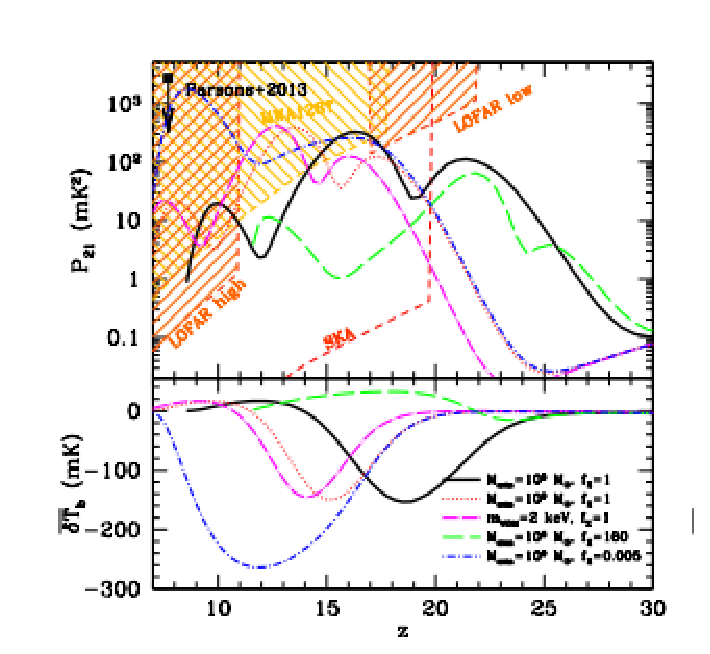
\includegraphics[width=0.5\hsize]{EoR/c03/c03.s2.f15.eps}
% \caption{(top)$z$$B$N4X?t$H$7$F8+$?;~$N(B21cm$B%Q%o!<%9%Z%/%H%k(B(fiducial model$B$O9u@~(B)$B$H(BMWA, LOFAR, SKA$B$N%N%$%:6J@~!#(B(bottom)$B51EY29EY$N(B$z$$B?J2=!#(B}
% \label{bukuro.constraining.fig:fig1}
% \end{figure}

\subsubsection{$B=i4|6d2O$N(BX$B@~J|<M$N@-<A(B}
$B=iBe6d2O$+$i$N(BX$B@~J|<M$O(BIGM$B$N29EY$r(BCMB$B29EY$h$j$b9b$$29EY$^$G>e>:$5$;$k$b(B
$B$N$H9M$($i$l$F$*$j!"(BIGM$B$N%$%*%s2=3d9g$,?t(B$\%$$BDxEY$N$H$-!"(BX$B@~J|<M$N%(%M%k(B
$B%.!<$N$[$H$s$I$,(BIGM$B$N2CG.$K$D$.9~$^$l$k!#(BX$B@~J|<M$O%$%*%s2=$h$j$b2CG.8;$H(B
$B$7$F8z2LE*$G$"$k!#$7$+$7!"4V@\E*$K$O$G$O$"$k$,!"(BX$B@~J|<M$K$h$C$F%8!<%s%:(B
$B<ANL$,>e$,$j!"8w;R2CG.$N%U%#!<%I%P%C%/$,CY$l$k$3$H$K$h$C$F:FEEN%$rCY$i$;(B
$B$k$H$$$&8z2L$b$"$k(B \citep{2013MNRAS.431..621M}$B!#(BX$B@~J|<M$H(BIGM$B$NAj8_:nMQ$O(B
$B$=$NBg$-$JJ?6Q<+M39TDx$K$h$C$FFCD'IU$1$i$l$k!J<0(B.\ref{eq:mfp}$B!K!#(B 
\begin{equation}
\lambda_{X}\sim 20 \overline{x}_{{\rm HI}}^{-1}\left(\frac{E_{X}}{300{\rm eV}}\right)^{2.6}\left(\frac{1+z}{10}\right)^{-1}c{\rm Mpc}
\label{eq:mfp}
\end{equation}
$\overline{x}_{{\rm HI}}$$B$OJ?6QCf@-?eAGN($G$"$j!"(B$E_{X}$$B$O8w;R$N%(%M%k%.!<(B
$B$G$"$k!#$3$N<0$h$j!"Fp(BX$B@~J|<M(B($E_{X}\le {\rm keV}$)$B$,(BIGM$B$HAj8_:nMQ$7!"(B
21cm$B@~$N8&5f$H7k$S$D$/;v$,J,$+$k!#(BIGM$B$N2CG.$K$h$k1F6A$O(B21cm$B%Q%o!<%9%Z%/(B
$B%H%k$N#2$DL\$N%T!<%/$KI=$l$k$,!"(BSKA1$B$G$O$3$N;~4|$N(B21cm$B%Q%o!<%9%Z%/%H%k$O(B
$B4QB,2DG=$HM=A[$5$l$F$$$k(B($B?^(B\ref{KH4})$B!#(B
%$B?^(B\ref{bukuro.constraining.fig:fig1}$B!K(B 

\subsubsection{$B2CG.4|$N(B21cm forest}
IGM$B$N29EY$,(BCMB$B29EY$h$j$b9b29$K2CG.$5$l$k0JA0$K$O!"9b@VJ}JP0\$NGX7JEEGH8;(B
$B$+$i$N8w$r(BIGM$B$,5[<}$9$k$3$H$K$h$j!"(B21 cm$B5[<}@~$,4QB,$5$l$k!#$3$l$r(B
Ly$\alpha$ forest$B$H$N%"%J%m%8!<$G(B21 cm forest$B$H8F$V!#(BSKA$B$G$b$3$N(B21 cm
forest$B$r4QB,$G$-$k$+$OFq$7$$$H$5$l$F$$$k(B \citep{2012MNRAS.425.2988M}$B!#:G(B
$BBg$NLdBj$H$7$F5s$2$i$l$k$N$OEEGH$r6/$/H/$9$k%/%'!<%5!<$J$I$NGX7JEEGH8;$,(B
$B9b@VJ}JP0\$G$bB8:_$9$k$+$H$$$&$3$H$G$"$k!#$7$+$7!"0E$$%/%'!<%5!<$G$bE}7W(B
$BE*<jK!$rMQ$$$l$P!"(B21cm forest$B$N8z2L$r2CG.4|A0$N(B21cm$B%Q%o!<%9%Z%/%H%k$N>.(B
$B%9%1!<%k$G8+$i$l$k2DG=@-$,$"$k(B \citep{2014MNRAS.441.2476E}$B!#(B21 cm$B%Q%o!<%9(B
$B%Z%/%H%k$NBg%9%1!<%k$O(BX$B@~$rJ|<M$9$k6d2O$K$h$k29EYMI$i$.$,;YG[E*$G$"$k$,!"(B
$B>.%9%1!<%k$G$O9b@VJ}JP0\$NEEGH$r6/$/H/$9$k(BAGN$B$J$I$,8z$$$F$/$k$N$G!"9b@V(B
$BJ}JP0\$N(BAGN$B$N<oB2$X$N@)8B$J$I$,4|BT$5$l$F$$$k!#(B 

\subsubsection{EoR$B%=!<%9(B}
EoR$B$N;~4|$d4|4V$NB>$K!"(B21cm$B%7%0%J%k$O(BEoR$B%=!<%9<+BN$K$D$$$F$b8@5Z$G$-$k!#(B
EoR$B$O8=:_$N4QB,$d>-Mh4QB,$N46EY8B3&$r2<2s$kbd>.6d2O$K$h$C$F0z$-5/$3$5$l(B
$B$k$H9M$($i$l$F$$$k$,!"$3$N$h$&$J9b@VJ}JP0\$Nbd>.6d2OFb$G$N@17A@.8zN($OITDj(B
$B@-$,Bg$-$/!"%U%#!<%I%P%C%/2aDx$b$h$/J,$+$C$F$$$J$$!#$7$+$7!"%U%#!<%I%P%C(B
$B%/8z2L$,@17A@.8zN($N?J2=$rD4@0$9$k$H9M$($i$l$F$*$j!"%U%#!<%I%P%C%/$NMM;R(B
$B$rCN$k;v$O(BEoR$B%=!<%9$rCN$k>e$G=EMW$G$"$k!#$3$l$rCN$k<j$,$+$j$N0l$D$H$7$F(B
EoR$B$N4v2?3XE*FCD'$r4QB,$9$k$H$$$&J}K!$,$"$k!#%$%*%s2=$r5/$3$7$F$$$k9=B$(B
$B$h$j$b>.%9%1!<%k$N(BEoR$B$N4v2?3XE*FCD'$r4QB,$9$k;v$K$h$j!"(BEoR $B%=!<%9$,$I$N(B
$B$h$&$K%O%m!<$H7k$S$D$-!"@17A@.8zN($K1F6A$rM?$($k$N$+$rCN$k;v$,$G$-$k$H9M(B
$B$($i$l$k!#(B 
%HIデータを用いたCDとEoRへの制限
\subsection{$B%P%j%*%s$H%@!<%/%^%?!<$NAjBPB.EY(B} 
\label{c03.s2.ss8}

$B1'Ch$N@2$l>e$,$j0J9_$N%P%j%*%s$NL)EY$f$i$.$N;~4VH/E8$dG.;K$O!"=iBeE7BN(B
$B!J=iBe@1!&=iBe6d2O!K7A@.2aDx$K$*$$$F=EMW$JLr3d$r2L$?$9!#FC$K!"=iBeE7BN$+(B
$B$i$NmU<M$O!"1'Ch$N:FEEN%$r5/$3$71'Ch0E9u;~Be$d$=$N8e$NE7BN7A@.$KBg$-$J1F(B
$B6A$rM?$($k$?$a!"1'Ch@2$l>e$,$j0J9_$N9=B$7A@.$rM}O@E*$KM}2r$9$k$3$H$O6K$a(B
$B$F=EMW$G$"$k!#(B

$B6aG/!"1'Ch@2$l>e$,$j0J9_$K$*$1$k%P%j%*%s$H%@!<%/%^%?!<$NAjBPB.EY$,9=B$7A(B
$B@.$dE7BN7A@.$KM?$($k1F6A$,(B\citet{2010PhRvD..82h3520T}$B$K$h$C$F;XE&$5$lCmL\(B
$B$r=8$a$F$$$k!#E57?E*$JAjBPB.EY$OFs>hJ?6Q$G(B30km/s$BDxEY$H$J$j!"@2$l>e$,$jD>(B
$B8e$N2;B.(B(6km/s)$B$rBg$-$/>e2s$kD62;B.$JAjBPB.EY$,IaJWE*$KB8:_$9$k!#$3$l$^$G(B
$B$NM}O@E*$J8&5f$G$O!"%P%j%*%s$H%@!<%/%^%?!<$NAjBPB.EY$K$h$k9=B$7A@.$KBP$9(B
$B$k1F6A$O#2<!$N8z2L$G$"$j!"$"$^$jCmL\$5$l$FMh$J$+$C$?$,!"%P%j%*%s$H%@!<%/(B
$B%^%?!<$K$3$N$h$&$JBg$-$JAjBPB.EY$,B8:_$9$k>u67$G$O!"=i4|$KAjBPB.EY$,$J$$(B
$B>l9g$HHf3S$7$F%@!<%/%^%?!<%O%m!<$N?tL)EY$d$=$NFbIt$N%P%j%*%s%U%i%/%7%g%s(B
$B$,>.$5$/$J$k$3$H$,(B\citet{2012ApJ...747..128N, 2013ApJ...763...27N}$B$N8&5f(B
$B$GL@$i$+$H$J$j!"%P%j%*%s$H%@!<%/%^%?!<$NAjBPB.EY$K$h$kE7BN7A@.$KBP$9$k1F(B
$B6A$K$D$$$F$N8&5f$,(B2010$BG/0J9_$K@9$s$K$J$C$F$-$F$$$k!#(B


$B%P%j%*%s$H%@!<%/%^%?!<$NAjBPB.EY$K$h$C$F1F6A$r<u$1$k%@!<%/%^%?!<%O%m!<$N(B
$B<ANL%9%1!<%k$O$=$N;~!9$N(BJeans$BD9$d(BJeans$B<ANL$N;~4VJ?6Q$KAjEv$9$k(B
filtering mass$B$N%9%1!<%k$G$"$j!"6qBNE*$K$O<g$K(B$10^5M_{\odot}$$B!A(B
$10^7M_{\odot}$$B$N%@!<%/%^%?!<%O%m!<$N7A@.$K1F6A$,=P$k!#$3$N%9%1!<%k$N%@!<(B
$B%/%^%?!<%O%m!<$O=iBe@1$d=iBe6d2O$KBP1~$7!"AjBPB.EY$N%3%R!<%l%s%9%9%1!<%k(B
$B$O%P%j%*%s2;6A?6F0$N%9%1!<%k(B($108h^{-1}$Mpc)$B$H$[$\F1$8$G$"$k$?$a!"1'Ch:F(B
$BEEN%4|$*$1$kE7BN7A@.$d:FEEN%$=$N$b$N$KBP$7$FBg$-$J%$%s%Q%/%H$rM?$($k$HM=(B
$BA[$5$l!"I,A3E*$K(BSKA$B$K$h$kCf@-?eAG(B21cm$B@~$N4QB,$,%P%j%*%s$H%@!<%/%^%?!<$NAj(B
$BBPB.EY$,E7BN7A@.$K5Z$\$91F6A$K$D$$$F$NCN8+$rF@$k6/NO$J<jCJ$H$J$k!#(B

$B1'ChO@E*$J9=B$7A@.$N?tCM%7%_%e%l!<%7%g%s$rMQ$$$F!"%P%j%*%s$H%@!<%/%^%?!<(B
$B$NAjBPB.EY$,:FEEN%4|$NE7BN7A@.$K5Z$\$91F6A$rD4$Y$k8&5f$,J#?t$N8&5f%0%k!<(B
$B%W$G9T$o$l$F$$$k(B
\citep{2011MNRAS.412L..40M,2012ApJ...747..128N,2013ApJ...763...27N}$B!#?^(B
\ref{c6.s3.ss5.f1}$B$O@VJ}JP0\(B$23$$B$H(B$19$$B$K$*$$$F7A@.$5$l$?%,%9%/%i%&%I$N<ANL4X(B
$B?t$r<($7$?$b$N$G!"B.EY:9$N1F6A$H$7$F%,%9%/%i%&%I$N<ANL$H?tL)EY$,2<$,$k79(B
$B8~$,L@3N$K$o$+$k!#B.EY:9$,(B$60$ km/s$B$N>l9g$N%,%9%/%i%&%I$N<ANL4X?t$O!"(B
$\sigma_8$$B$r(B$0.9$$B$+$i(B$0.8$$B$K2<$2$?>l9g$HF1DxEY$N1F6A$,$"$k!#;~4V$,7P$D$H!"B.(B
$BEY:9$,>.$5$/$J$k$?$a$KB.EY:9$NM-L5$K$h$k<ANL4X?t$X$N1F6A$O>.$5$/$J$k798~(B
$B$,8+$i$l$k!#@VJ}JP0\(B$19$$B$K$*$$$F$O!"B.EY:9$NM-L5$K$h$C$F<ANL4X?t$K(B2$BG\DxEY$N(B
$B0c$$$,8+$i$l$?$,!"@VJ}JP0\(B$10$$B$G$OB.EY:9$NM-L5$K$h$k<ANL4X?t$X$N1F6A$O$h$j(B
$B8BDjE*$H$J$j(B$10$\%$BDxEY$H$J$k!#$^$?!"0lC6%,%9%/%i%&%IFb$G$N@17A@.$,;O$^$k$H!"(B
$BAjBPB.EY$N1F6A$O7A@.$5$l$k=iBeE7BN$N7A@.N(!&EEN%8w;R$K$h$k:FEEN%!&=E85AG(B
$B6!5k$J$I$KGH5Z$9$k!#AjBPB.EY$NBg$-$JNN0h$G$O!"@17A@.N($N?d0\$,B>$NNN0h$h(B
$B$j$bCY1d$7!"$=$l$KH<$C$F:FEEN%$d=E85AG6!5k$bCY1d$9$k(B($B?^(B
\ref{c6.s3.ss5.f2})$B!#$3$N7k2L!"AjBPB.EY>l$N%3%R!<%l%s%9%9%1!<%k$GEEN%EY$N(B
$B6u4VE*JQF0$,H/@8$7!"(B21 cm$B@~J|<M$N6u4VJ,I[$N%Q%o!<%9%Z%/%H%k$KH?1G$5$l$k$H(B
$BM=A[$5$l$k!#(B

\begin{figure}[!t]
 \centering \includegraphics[width=0.9\linewidth] {EoR/c03/c03.s2.f16.eps}
 \caption{$B@VJ}JP0\(B23($B>eCJ(B)$B$H(B19($B2<CJ(B)$B$K$*$1$k%,%91@$N<ANL4X?t!#:8$H1&$O$=(B
 $B$l$>$l(Bdifferential$B$J<ANL4X?t$H(Bcumulative$B$J<ANL4X?t!#(B
 \label{c6.s3.ss5.f1}}
\end{figure}
\begin{figure}[!h]
 \centering \includegraphics[width=10cm] {EoR/c03/c03.s2.f17.eps}
 \caption{$B>eCJ!'%P%j%*%s$H%@!<%/%^%?!<$NAjBPB.EY$NBP$9$k(BPop-III$B$HA4BN$N@1(B
 $B7A;K$N;~4VH/E8!#2<CJ!'(BPop-III$B$N7A@.N($NA4BN$N@17A@.N($KBP$9$k4sM?$N;~4VH/E8!#(B
 \label{c6.s3.ss5.f2}}
\end{figure}


SKA$B$N4QB,7k2L$r@5$7$/2r<a$9$k$K$O!"%P%j%*%s$H%@!<%/%^%?!<$NAjBPB.EY$K$h$k(B
$B9=B$7A@.$X$N1F6A$rDjNLE*$K8+@Q$b$k$3$H$,I,MW$G$"$k!#@VJ}JP0\$,(B$20$$B0J>e$N@1(B
$B7A@.3hF0$,;O$^$C$F$$$J$$;~4|$N4QB,$K$O!"%,%9%/%i%&%I$KK-IY$K4^$^$l$k(B
H$_2$$B$d(BHD$B$H$$$C$?J,;R$N2sE>A+0\J|<M$,%,%9$NJ,I[$NNI$$%H%l!<%5!<$H$J$k!#(B
H$_2$$B$N(B$J=2\rightarrow 0$$B$N2sE>A+0\!"(BHD$B$N(B$J=4\rightarrow 3$$B$N2sE>A+0\$,=P(B
$B$9(B$533$ GHz$B$NJ|<M$O@VJ}JP0\(B$35\sim 40$$B$G$"$l$P!"(B$14$ GHz$B$^$G4QB,$G$-$k(BPhase-1$B$N(B
SKA-MID $B$G4QB,2DG=$G$"$k!#99$K(B $24$ GHz$B$^$G4QB,2DG=$G$"$k(BPhase-2$B$G$"$l$P!"@V(B
$BJ}JP0\(B$20$$BDxEY$^$G4QB,2DG=$G$"$k!#$^$?!"=iBeE7BN$,7A@.$5$l1'Ch:FEEN%$,?J$`(B
$B2aDx$G$N%P%j%*%s$H%@!<%/%^%?!<$NAjBPB.EY$N1F6A$r4QB,$9$k$K$O!"Cf@-?eAG$N(B
21 cm$B@~$r%H%l!<%5!<$H$7$F@VJ}JP0\(B$6<z<20$$B$NCf@-?eAG$+$i$NJ|<M$r(B$50 \sim 350$
MHz
$B$N<~GH?tBS$r%+%P!<$9$k(BSKA-low$B$,:GE,$G$"$k!#(B

%バリオンとダークマターの相対速度
\subsection{EoR/Cosmic Dawn$B4|$N1'ChO@(B}
\label{c03.s2.ss9}

$B6aG/!"(BWMAP, Planck$B$r$O$8$a$H$9$k1'Ch%^%$%/%mGHGX7JmU<M(B(CMB)$B29EYMI$i$.$dJP(B
$B8w$N4QB,!"$^$?(BSDSS$B$r$O$8$a$H$9$kBg5,LO6d2O%5!<%Y%$$K$h$k!"1'Ch$N9=@.MWAG(B
$B$dMI$i$.$N=i4|>r7o$rM?$($k%$%s%U%l!<%7%g%sM}O@$r5-=R$9$k1'ChO@%Q%i%a!<%?(B
$B$N@:L)B,Dj$,2DG=$H$J$j!"1'ChO@$O@:L)2J3X$H$7$F3NN)$5$l$F$-$F$$$k!#(B

$B$7$+$7$^$@$^$@!"%@!<%/%^%?!<!"%@!<%/%(%M%k%.!<$N@5BN$d%K%e!<%H%j%N<ANL$J(B
$B$I2r7h$9$Y$-LdBj$,B8:_$9$k!#>-Mh4QB,$K$*$1$k$3$l$i$NLdBj2r7h$KBP$9$k%"%W(B
$B%m!<%A$H$7$F$O!"C1=c$K$O;~4V!"6u4VE*$K$h$jI}9-$$4QB,$r9T$&$3$H$G$"$k!#(B

SKA$B$O!"0J>e$N$h$&$J8=:_$N1'ChO@$K$*$1$kLdBj2r7h$K$H$C$FHs>o$K=EMW$J0LCV$r(B
$B@j$a$F$$$k!#$3$l$^$G4QB,$7$?$3$H$N$J$$!";~4VE*$K$O9b@VJ}JP0\1'Ch$N>pJs$r(B
$BM?$($F$/$l$k$@$m$&$7!"6u4VE*$K$O$h$j>.$5$J%9%1!<%k$^$G4QB,$G$-$k$+$i$G$"(B
$B$k!#(B

\paragraph{$BL)EYMI$i$.$N>pJs$rMQ$$$?1'ChO@%Q%i%a!<%?$X$N@)8B(B}

SKA$B$O!"(B21cm$B51EY29EY!J(B21cm$B%7%0%J%k!K$rL)EY>l$NDI@W;R!J%H%l!<%5!<!K$H$7$F;H$$!"(B
$B1'ChO@%Q%i%a!<%?$KBP$7$F@)8B$rM?$($k$3$H$,=PMh$k!#(B

$B$3$N51EY29EY$O!"%9%T%s29EY!"Cf@-?eAG$N3d9g$HL)EY>l$K0MB8$9$k!#(B
$BFC$K%9%T%s29EY$,(BCMB$B29EY$KHf$Y$FHs>o$K9b$$>l9g!"(BCMB$B29EY$+$i$_$?51EY29EY$O!"(B
$B$*$*$h$=(B
\begin{equation}
\delta T_B = (1 + \delta ) x_H \times \cdots
\end{equation}
$B$H=q$1$k!#(B$x_H$$B$,Cf@-?eAG$N3d9g$G!"(B$\delta$$B$,J*<A$NL)EY>l$rI=(B
$B$9(B~\citep{2006PhR...433..181F}$B!#FC$K(B$x_H = 1$$B$N>l9g$K$O(B$\delta T_B$$B$O!"L)(B
$BEY>l$NL5%P%$%"%9DI@W;R$H$J$k!#$3$N$h$&$JHs>o$KM}A[2=$5$l$?>u67$G$N%Q%i%a!<(B
$B%?7hDj@:EY$O!"(BSKA0 (SKA1$B$NH>J,$N%"%s%F%J$N?t(B)$B$G(B$z=7,7.5,8$$B$G$N51EY29EY$r(B
$B4QB,$7$?>l9g!"(BPlanck$B$H$[$\F1DxEY!"(BSKA2(SKA1$B$N#4G\$N%"%s%F%J$N?t(B)$B$G$O!"FC(B
$B$K>.%9%1!<%k$N>pJs$r$h$j@:L)$KB,Dj$9$k$3$H$,2DG=$H$J$k$N$G!"Nc$($P=i4|MI(B
$B$i$.%Q%o!<%9%Z%/%H%k$N%9%Z%/%H%k;X?t$NJQ2=(B(running spectral index)$B$d%K%e!<(B
$B%H%j%N<ANL$N7hDj@:EY$,(BPlanck$B$KHf$Y%U%!%/%?!<#3DxEY2~A1$9(B
$B$k(B~\citep{2008PhRvD..78f5009P,2009PhLB..673..173B, 2011JCAP...02..021A}$B!#(B

\paragraph{$B!V1'ChO@E*MWAG!W$H!V1'ChJ*M}E*MWAG!W$NJ,N%(B}

$B$7$+$7<B:]$K$O!"$3$N$h$&$JM}A[E*$J>u67$K$O$J$C$F$*$i$:!"4QB,$5$l$k@VJ}JP(B
$B0\$G$N%,%929EY$J$I$5$^$6$^$J1'ChJ*M}E*$JMWAG$,(B$\delta T_B$$B$K$O:.F~$7$F$/(B
$B$k!#1'ChO@$H$3$N1'ChJ*M}E*$JMWAG$r40A4$KJ,N%$9$k$?$a$K$O!"1'ChJ*M}E*8z2L(B
$B$KBP$9$kM}O@%b%G%k$N9=C[$,$^$:9M$($i$l$k(B~\citep{2008PhRvD..78b3529M}$B!#$b$&(B
$B$R$H$D$O!"(B$\delta T_B$$B$N%Q%o!<%9%Z%/%H%k$K$*$1$k@VJ}JP0\OD$_$rMQ$$$k$3$H(B
$B$G$"$k!#$3$N@VJ}JP0\OD$_$O!"%I%C%W%i!<%7%U%H$K5/0x$9$k$,4QB,E*$K$O%Q%o!<(B
$B%9%Z%/%H%k$r3QEY0MB8@-$GE83+$7$?:]$K9b<!%b!<%a%s%H$H$7$FM?$($i$l$k!#FC$K(B
$B%X%-%5%G%+%]!<%k$O1'ChJ*M}E*8z2L$,F~$i$J$$L)EY>l$N$h$$DI@W;R$H$7$F9M$($i(B
$B$l!"$3$N9b<!%b!<%a%s%H$N4QB,$b=EMW$H9M$($i$l$k(B~\citep{2006ApJ...653..815M,2008PhRvD..78b3529M}$B!#(B

\paragraph{$B6d2O4V%,%929EY$N>pJs$rMQ$$$??7J*M}$NC5::(B}

$BL)EY>l$NDI@W;R$H$7$F>e$G$O(B21cm$B%7%0%J%k$r9M$($F$-$?$,!"@h$K$b=R$Y$?$h$&$K(B
21 cm$B%7%0%J%k$O!"1'Ch$N%$%*%s2=N($d6d2O4V%,%9(B(inter galactic medium
(IGM))$B$N29EY$K$b0MB8$9$k!#I8=`1'Ch%b%G%k$K$*$1$k9=B$7A@.%7%J%j%*$K4p$E$$(B
$B$?!"%$%*%s2=N($d(BIGM$B$N>uBV$N;~4VJQ2=$K2C$($F!"$5$i$K$3$l$i$N?J2=$,JQ99$r<u(B
$B$1$k$h$&$J?7$?$J%7%J%j%*$,$"$l$P!"(B21 cm$B%7%0%J%k$N4QB,$O9b@VJ}JP0\1'Ch$K$*(B
$B$1$k?7$?$JJ*M}$X$N@)8B$rM?$($k$b$N$H$7$F=EMW$G$"$k!#(B

$B$^$:$=$N$h$&$J8uJd$H$7$F!"0E9uJ*<A$N@-<A$,>e$2$i$l$k!#I8=`E*$JNd$?$$0E9u(B
$BJ*<A!J(BCDM$B!K%b%G%k$H$O0[$J$j!"<ANL$,Hf3SE*7Z$$$h$&$J$$$o$f$kCH$+$$0E9uJ*<A(B
 (Warm Dark Matter(WDM)) $B$,$7$P$7$P5DO@$5$l$F$$$k!#$3$N(BWDM$B%b%G%k$G$O!">.%9(B
$B%1!<%k9=B$$N7A@.$,M^@)$5$l!"6d2O7A@.$,I8=`E*$JNd$?$$0E9uJ*<A$N>l9g$h$jCY(B
$B$/$J$k!#7k2L$H$7$F!"(B21 cm$B%7%0%J%k$K$*$$$F!"1'ChJ*M}E*MWAG$,1F6A$rM?$($k;~(B
$B4|$,JQ99$r<u$1$k$N$G4QB,$+$i$3$N(BWDM$B%7%J%j%*$K@)8B$rM?$($k$3$H$,$G$-$k$H4|(B
$BBT$5$l$k(B~\citep{2014MNRAS.438.2664S}$B!#(B


$B$^$?0E9uJ*<A$NBP>CLG$dJx2u$r9M$($k$H!"$=$l$O(BIGM$B$rCH$a$k8z2L$H$7$FF/$-!"(B
IGM$B29EY$N;~4V?J2=$NMM;R$,I8=`%b%G%k$H$O0[$J$C$F$/$k!#$3$N$h$&$J(BIGM$B29EY$N(B
$B;~4VJQ2=$rDL$8$??7$?$J%b%G%k$X$N@)8B$K$H$C$F$b(B21cm$B%7%0%J%k$OM-8z$G$"(B
$B$k(B~\citep{2014JCAP...11..024E}$B!#(B

$BB>$K$b!"=i4|<'>l$d!"86;O%V%i%C%/%[!<%k$J$I$N!VJQ$o$C$?FC@-$r;}$C$?J*<A!W(B
$B$KBP$9$k@)8B$H$7$F$b(BSKA$B$K$h$k(B21cm$B4QB,$O=EMW$G$"$k$H9M$($i$l(B
$B$k(B~\citep{2014PhRvD..89j3522S}$B!#(B 

\paragraph{$B%P%k%/%U%m!<(B}

$B>\:Y$O(B``Bulk flows and the end of dark ages''$B$G?($l$k$,!"(Bbaryon$B$H0E9uJ*<A(B
$B$N4V$NB.EY>l$N0c$$$,9=B$7A@.$K1F6A$rM?$($k$3$H$,!";XE&$5$l$F$$(B
$B$k(B~\citep{2010PhRvD..82h3520T}$B!#$3$NAjBPB.EY$N1F6A$H$7$F$O!">.%9%1!<%k$N9=(B
$BB$7A@.$NM^@)$J$I$,9M$($i$l$k!#$3$N8z2L$O!"(B21 cm$B%7%0%J%k$GC5$k9b@VJ}JP0\1'(B
$BCh$G82Cx$G$"$k$N$G!"(BSKA$B$GC5$k?7$?$J1'ChO@E*8z2L$H$7$F5DO@$5$l$F$$$k!#(B


\paragraph{$B$=$NB>(B}

\begin{itemize}

\item $B=i4|Hs%,%&%9@-(B

$B=i4|6JN(MI$i$.$NE}7WJ,I[$O!"MI$i$.$N<o$H$J$k%9%+%i!<>l$NAj8_:nMQ$d>l$NMI$i$.$r6JN(MI$i$.$X$HE>49$9$k:]$NHs@~7A8z2L$K$h$j%,%&%9J,I[$+$i$o$:$+$K$:$l$k2DG=@-$,$"$k$3$H$,;XE&$5$l$F$$$k!#$3$N$h$&$J>l9g!"Hs>o$KBg$-$J%9%1!<%k$G$N6d2OJ,I[$,1F6A$r<u$1$F(B
$B%,%&%9J,I[$N;~$H$O0[$J$k%Q%o!<%9%Z%/%H%k$N?6$kIq$$$,8+$i$l$k!#1'Ch:FEEN%4|$N(B21cm$B%7%0%J%k$K$O!"(B
$B%$%*%s2=N($N>pJs$,F~$C$F$$$k$,!"$3$N%$%*%s2=N($,6u4VJ,I[$7$F$$$k>l9g!"(B21cm$B51EY29EY$N%Q%o!<%9%Z%/%H%k$O!"$=$NJ,I[$K0MB8$9$k!#6d2OJ,I[$HF1$8$h$&$K!"$3$N%$%*%s2=N($NJ,I[$K$b=i4|MI$i$.$NHs%,%&%9@-$O1F6A$rM?$($k$N$G!"(BSKA$B$J$I$K$h$j=i4|MI$i$.$NHs%,%&%9@-$K@)8B$rM?$($k$3$H$,=PMh$k!#(B
Planck$B$K$h$k(BCMB$B4QB,$GF@$i$l$F$$$k$3$NHs%,%&%9@-$KBP$9$k@)8B$HF1DxEY$N@)8B$rM?$($k$H4|BT$5$l$F$$$k(B~\citep{2011PhRvL.107m1304J}$B!#(B


\item $B1'ChO@E*=ENO%l%s%:8z2L(B

$B9b@VJ}JP0\$GH/$;$i$l$?(B21cm$B%7%0%J%k$O2f!9$KFO$/$^$G$K1'ChBg5,LO9=B$$rDL2a$7$F$/$k$N$G$=$N=ENO>l$N1F6A$K$h$C$F%l%s%:8z2L$r<u$1$k!#$3$N%l%s%:8z2L$rCj=P$G$-$l$P!"$"$i$?$J1'ChBg5,LO9=B$$N(Bprobe$B$H$7$F4|BT$G$-$k!#(BSKA$B$G$O==J,B,Dj2DG=$G$"$k$H9M$($i$l$F$$$k(B~\citep{2006ApJ...653..922Z,2006astro.ph.11862B}$B!#(B

\end{itemize}

\paragraph{$B$^$H$a(B}

SKA$B!J(BSKA-Low$B!K$O!"@VJ}JP0\$r<u$1$?Cf@-?eAG$N(B21cm$B@~%7%0%J%k$rB*$($k$3$H$G(B
$z = 6 - 27$$B$H$$$&9b@VJ}JP0\1'Ch$N;Q$rL@$i$+$K$9$k$H4|BT$5$l$F$$$k!#$3$N4QB,$K$h$j!"$3$l$^$G$N1'ChO@%Q%i%a!<%?$N7hDj@:EY$,8~>e$9$k$@$1$G$J$/!"0E9uJ*<A$N@-<A$J$I?7$?$JJ*M}$K4QB,E*$KGw$k$3$H$,$G$-$k$H4|BT$5$l$F$$$k!#(B


%Cosmology from EoR/Cosmic Dawn
\subsection{$B1'ChO@E*4QB,$HCf@-?eAG(B21~cm$B@~$NAj8_Aj4X(B}%\label{c6.s2}
\label{c03.s2.ss10}

SKA$B7W2h$K$*$$$F!"(BCosmic Dawn~(CD)$B$d(BEpoch of Reionization~(EoR)$B5/8;$N1'Ch(B
$BO@E*$JCf@-?eAG(B21~cm$B@~$N8!=P$O=EMW$J%-!<%5%$%(%s%9$N0l$D$G$"$k!#$7$+$7$J$,(B
$B$i!"$=$N4QB,GHD9BS$OE7$N@n6d2O$d6aK56d2O$K$"$k6/$$EEGH8;!"CO5e$NEEN%AX$N(B
$B1F6A!"$=$7$F%i%8%*GH$N43>D$J$I$K$h$j7h$7$FM}A[E*$J4QB,>r7o$H$O8@$($J$$!#(B
$B$9$J$o$A!"1'ChO@E*(B21~cm$B$N%7%0%J%k$O$3$l$i(B''$B%N%$%:(B''$B$KKd$b$l$F$7$^$$!"$=$N(B
$B8!=P$O:$Fq$r6K$a$k!#$3$N$h$&$J:$Fq$5$r2sHr$9$kJ}K!$N0l$D$H$7$F!"B>$N4QB,(B
$B$H$NAj8_Aj4X$,5s$2$i$l$k!#Fs$D$NFHN)$J4QB,!J$b$7$/$OGHD9!K$NAj8_Aj4X$r$H(B
$B$l$P!"$=$l$>$l$N%7%9%F%^%F%#%C%/$J%N%$%:$O$*8_$$BG$A>C$79g$$!"%N%$%:$KKd(B
$B$b$l$F$$$?%7%0%J%k$N8!=P$,2DG=$H$J$k!#(B

CD$B$d(BEoR$B5/8;$N%7%0%J%k$r<h$j=P$9;v$rL\E*$H$7$?;~!"1'ChO@E*(B21~cm$B@~$HAj8_Aj(B
$B4X$r<h$kM-NO$J4QB,$H$7$F!"1'Ch%^%$%/%mGHGX7JJ|<M(B~(CMB)$B!"9b@VJ}JP0\$N6d2O(B
$BC5::!"$=$7$F!"6a@V30@~GX7JJ|<M(B~(NIRB)$B$,5s$2$i$l$k!#$3$N>O$G$O!"$3$l$i$N4Q(B
$BB,$H(BCD$B$d(BEoR$B$H$N4XO"@-!"$=$7$F!"1'ChO@E*(B21~cm$B@~$HAj8_Aj4X$r$H$k;v$K$h$C$F!"(B
$B$I$N$h$&$J(BCD$B$d(BEoR$B$K4X$9$k>pJs$K%"%/%;%9=PMh$k$+$K$D$$$F%l%S%e!<$r$9$k!#(B

	
\subsubsection{CMB$B$H$NAj8_Aj4X(B}

CMB$B29EY$f$i$.$N@:L)4QB,$K$h$j!"2f!9$O1'Ch$NMM!9$J>pJs$K%"%/%;%9$G$-$k!#(B
$B$=$l$O!"1'Ch:F%$%*%s2=%W%m%;%9$bNc30$G$O$J$$!#(BCMB$B8w;R$O!"<+M3EE;R$H$N;6Mp$N:]!"(B
$B%I%C%W%i!<%7%U%H$r<u$1$k(B~\citep{zeldovich}$B!#(B
EoR$B4|$K$O<+M3EE;R?t$,G|Bg$KA}$($k$?$a!"$3(B
$B$N%I%C%W%i!<%7%U%H$,(BEoR$B4|5/8;$N29EY$f$i$.$,@8$8$k%a%+%K%:%`$H$J$k!#(B
$B$3$N;v$+$i!"(BCMB$B$N29EY$f$i$.$K$O!"(BEoR$B4|$N<+M3EE;R$N?tL)EY(B($B%$%*%s2=EY$b4^$`(B)$B$H$=$N!JG.1?F0$b$7$/$O%P%k%/1?F0$N!KB.EY$N?J2=;K$,Kd$a9~$^$l$F$$$k$H8@$($k!#(B
$BBg$^$+$K8@$($P!"Bg%9%1!<%k$N29EY$f$i$.$K$O1'ChJ?6Q$N%$%*%s2=EY$,!">.%9%1!<(B
$B%k$G$O%$%*%s2=%P%V%k$K$h$C$F:n$i$l$k6I=jE*$J%$%*%s2=EY$,$=$l$>$lL)@\$K4X(B
$B$o$C$F$/$k(B ($B>\$7$$%l%S%e!<$H$7$F!"Nc$($P(B~\cite{2008RPPh...71f6902A}
$B$r8+$h(B)$B!#(B

$B$7$+$7$J$,$i!"(BEoR$B4|$K@8@.$5$l$k29EY$f$i$.$O29EY$f$i$.A4BN$G8@$($P>.$5$/!"(B
$BB>$N5/8;$N29EY$f$i$.$N@.J,$KKd$b$l$F$$$k!#$3$NKd$b$l$?%7%0%J%k$rIb$+$S>e$,$i$;(B
$B$kJ}K!$N0l$D$,!"(B21~cm$B@~$H(BCMB$B$NAj8_Aj4X$G$"$k!#$7$?$,$C$F!"3F!9$N<+8JAj4X$G$OKd$b$l(B
$B$F$7$^$C$F$$$k(BEoR$B$N>pJs$K%"%/%;%9$G$-$k2DG=@-$b$"$k$3$H$+$i!"$3$NAj8_Aj(B
$B4X$NJ*M}$NM}2r$N$?$a$K!"2r@OE*!"?tCM7W;;E*$NN>J}$NLL$+$iB?$/$N8&5f$,$J$5(B
$B$l$F$$(B
$B$k(B~\citep{2005MNRAS.360.1063S,2008MNRAS.384..291A,2004PhRvD..70f3509C,2006ApJ...647..840A,2007MNRAS.377..168S,2010MNRAS.402.2617T,2010MNRAS.402.2279J,2011MNRAS.414.3424T}$B!#(B
$B$=$N7k2L!"Bg$-$J%9%1!<%k$G$NAj8_Aj4X%7%0%J%k$NBg$-$5$O!"1'ChJ?6QE*$J(B
$B%$%*%s2=$N%9%T!<%I$K0MB8$9$k$3$H$,<($5$l$?!#%$%*%s2=$,5^7c$K?J$`$[$I!"$=$N(B
$B%7%0%J%k$NBg$-$5$OBg$-$/$J$k$N$G$"$k!#?^(B~\ref{fig:cmb_cross}$B$O(B~\cite{2010MNRAS.402.2617T} $B$K4p$E$$$F!":F%$%*%s2=%b%G(B
$B%kKh$N(B
Signal-Noise ratio~(S/N)~$B$rI=$7$?$b$N$G$"$k!#2#<4$O4QB,$N(Bsky~fraction$B!"(B
$B=D<4$O(B21~cm$B@~4QB,$N5,3J2=$5$l$?%N%$%:%Q%o!<$G$"$k!#$3$N?^$G$O!"(BCMB$B29EY$f$i$.$N(B
$B4QB,$H$7$F!"(BPlanck$B1R@1$N46EY$r:NMQ$7$F$*$j!"1'Ch$NJ?6Q%$%*%s2=EY$N?J2=$N%b%G(B
$B%k$H$7$F!"(B
\begin{equation}
x_e(z) = \frac{1}{1+\exp[(z-z_{\rm re})/\Delta z]},
\end{equation}
$B$r:NMQ$7$F$$$k!#(B
$B$3$N%b%G%k$G$O!"(B$\Delta z$$B$,>.$5$$$[$I%$%*%s2=$,5^7c$K?J$`!#$=$N$?$a!"Aj8_Aj(B
$B4X$N%7%0%J%k$bBg$-$/$J$k$N$G!"(BS/N$B$O>.$5$$(B$\Delta z$$B$[$IBg$-$/$J$k!#(B
$B8=:_7W2h$5$l$F$$$k3F(BSKA$B$N%G%6%$%s$O@VE@$G<($5$l$F$$$k!#$7$?$,$C$F!"(BSKA$B$G$NAj8_Aj4X$N%7%0%J%k$N8!=P!"L$8!=P$K$h$j:F%$%*%s2=%W%m%;%9$K$D$$$F@)8B$rM?$($k2DG=@-$,$"(B
$B$k$3$H$,$o$+$k!#(B


\begin{figure}[!t]
 \begin{minipage}{0.5\hsize}
  \begin{center}
   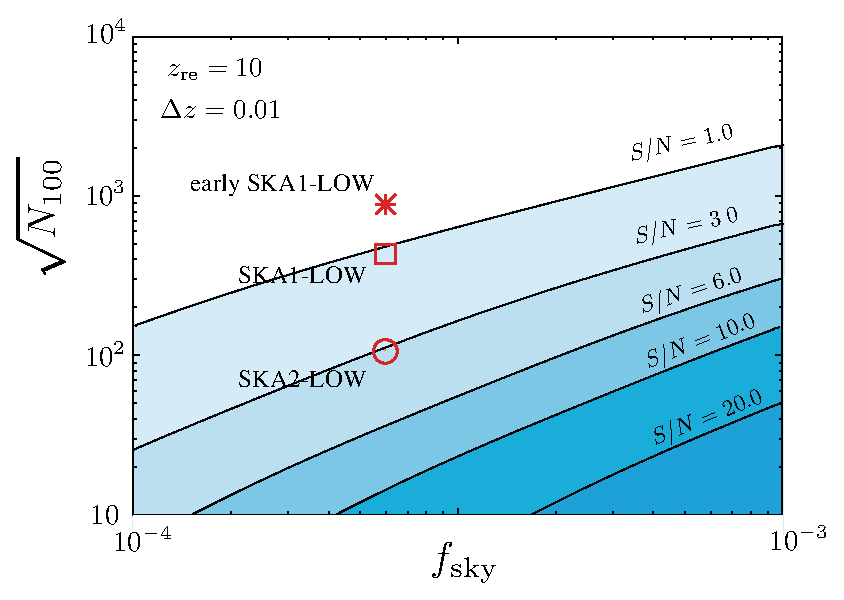
\includegraphics[width=70mm]{EoR/c03/c03.s2.f18.eps}
  \end{center}
 \end{minipage}
 \begin{minipage}{0.5\hsize}
  \begin{center}
   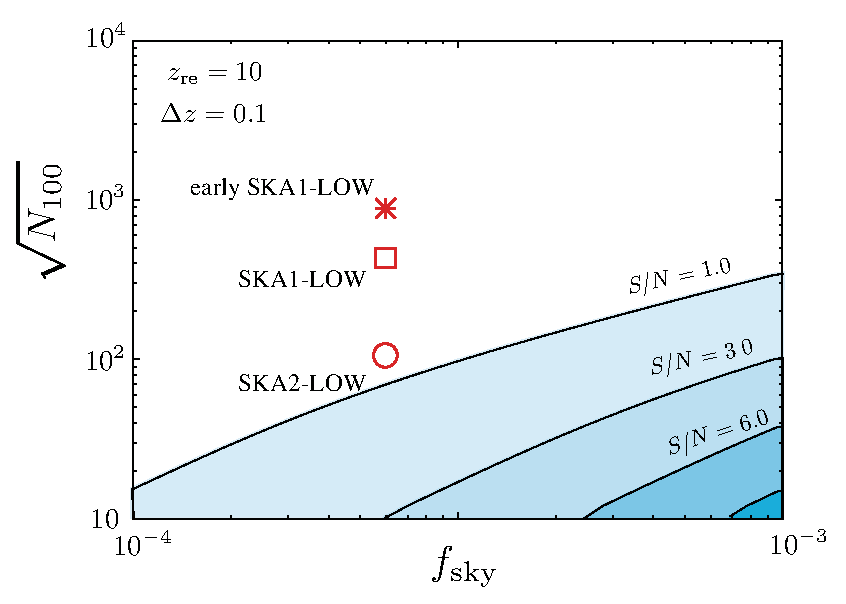
\includegraphics[width=70mm]{EoR/c03/c03.s2.f19.eps}
  \end{center}
 \end{minipage}
  \caption{$B:F%$%*%s2=%b%G%kKh$N(B21~cm$B$H(BCMB$B$NAj8_Aj4X$N(BS/N$BHf!#2#<4$O(B21~cm$B@~4QB,$N(B
 sky~fraction$B!"=D<4$OB?=E6K(B$\ell =100$$B$G5,3J2=$5$l$?4QB,$N%N%$%:%Q(B
 $B%o!<(B~($B%N%$%:$N3QEY%Q%o!<%9%Z%/%H%k(B$N(\ell)$$B$O(B$N(\ell )
 =N_{100}(\ell/100)^2$$B$GM?$($i$l$k(B)$B!#:8%Q%M%k$G$O(B$\Delta z = 0.01$$B!#(B
 $B1&%Q%M%k$G$O(B$\Delta z = 0.1$$B!#N>%Q%M%k$H$b(B$z_{\rm re} = 10$$B$G$"$j!"4QB,(B
 $B<~GH?t$O(B$z=10$$B$KBP1~$9$k!#(B}
  \label{fig:cmb_cross}
\end{figure}




\subsubsection{$B9b@VJ}JP0\6d2O$H$NAj8_Aj4X(B}

$B6d2O$OL)EY$f$i$.$N%H%l!<%5!<$G$"$k$HF1;~$K!"M-NO$J1'Ch:F%$%*%s2=8;$N0l$D(B
$B$H$7$F9M$($i$l$F$$$k!#$=$N$?$a!"1'ChO@E*(B21~cm$B@~$N%7%0%J%k$N6/$5$H6d2O$N(B
$B?tL)EY$H$NAj8_Aj4X$O!"1'Ch$N%$%*%s2=EY$K1~$8$F!"$9$3$7J#;($JMMAj$r<($9(B~\citep{2009ApJ...690..252L,2013MNRAS.432.2615W}$B!#(B

\begin{figure}[!t]
  \begin{center}
   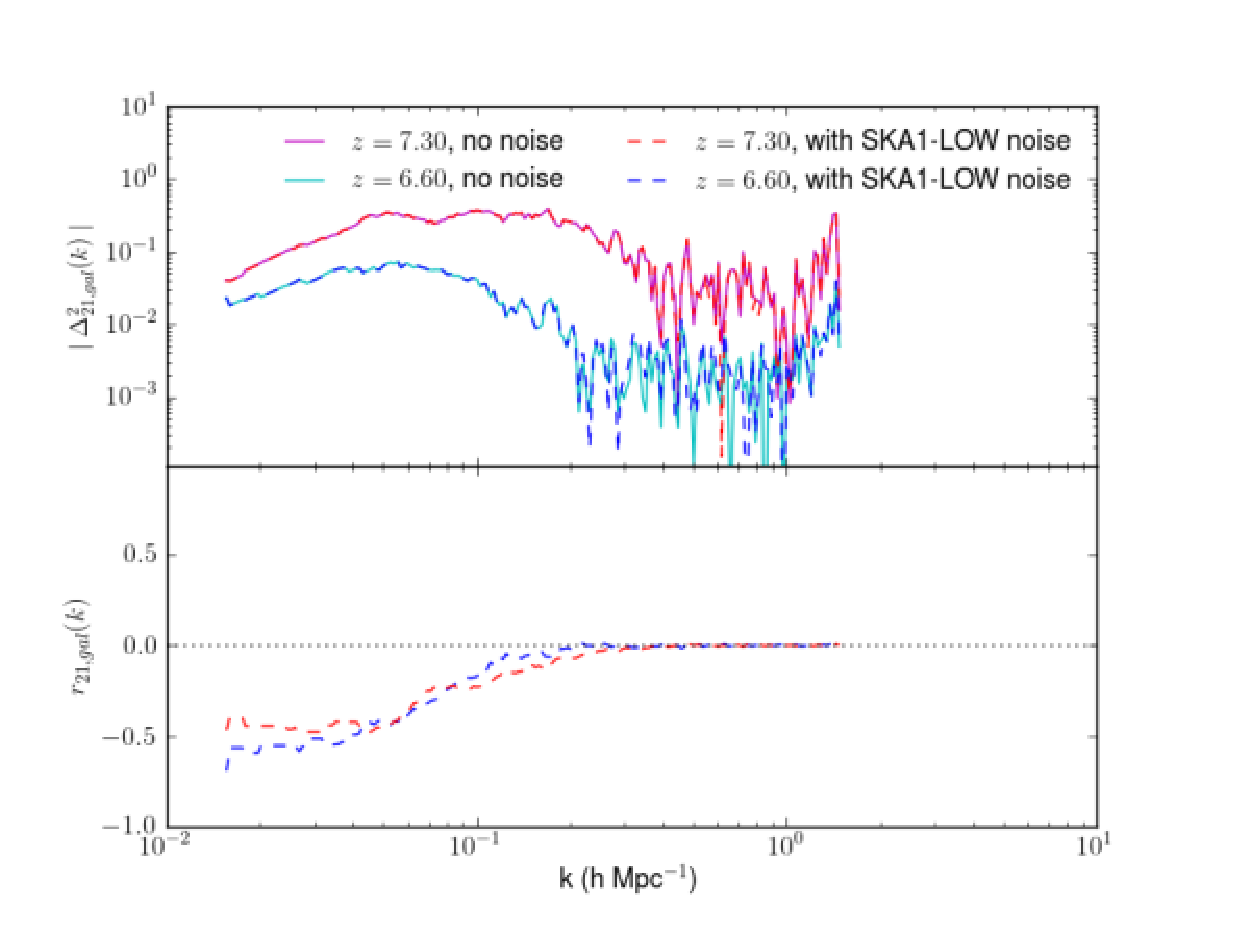
\includegraphics[width=100mm]{EoR/c03/c03.s2.f20.eps}
  \end{center}
 \caption{21~cm$B@~$H6d2O$NAj8_Aj4X$NL5<!852=$5$l$?%Q%o!<%9%Z%/%H%k!J>e%Q%M%k!K$H$=$NAj(B
 $B4X78?t!J2<%Q%M%k!K!#$3$3$GAj4X78?t(B$r$$B$O(B,$B6d2O$H(B21~cm$B@~$NL5<!85%Q%o!<%9%Z%/%H%k!"(B
 $\Delta^2(k)_{\rm halo}$$B$H(B$\Delta^2(k)_{21}$$B$rMQ$$$F!"(B
 $r=\Delta^2(k)_{21,\rm halo}/ \Delta^2(k)_{\rm halo} \Delta^2(k)_{21}$$B!#(B
 }
  \label{fig:galaxy_cross}
\end{figure}
\begin{figure}[!h]
 \begin{minipage}{0.5\hsize}
  \begin{center}
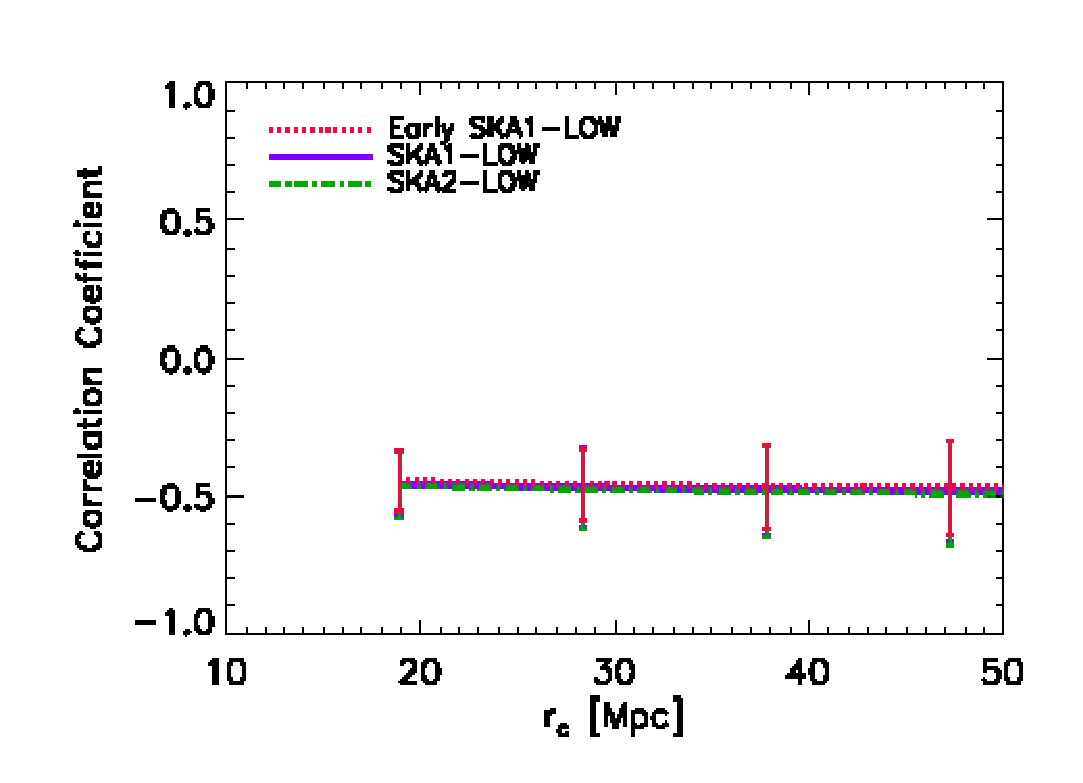
\includegraphics[width=70mm]{EoR/c03/c03.s2.f21.eps}
  \end{center}
 \end{minipage}
 \begin{minipage}{0.5\hsize}
  \begin{center}
   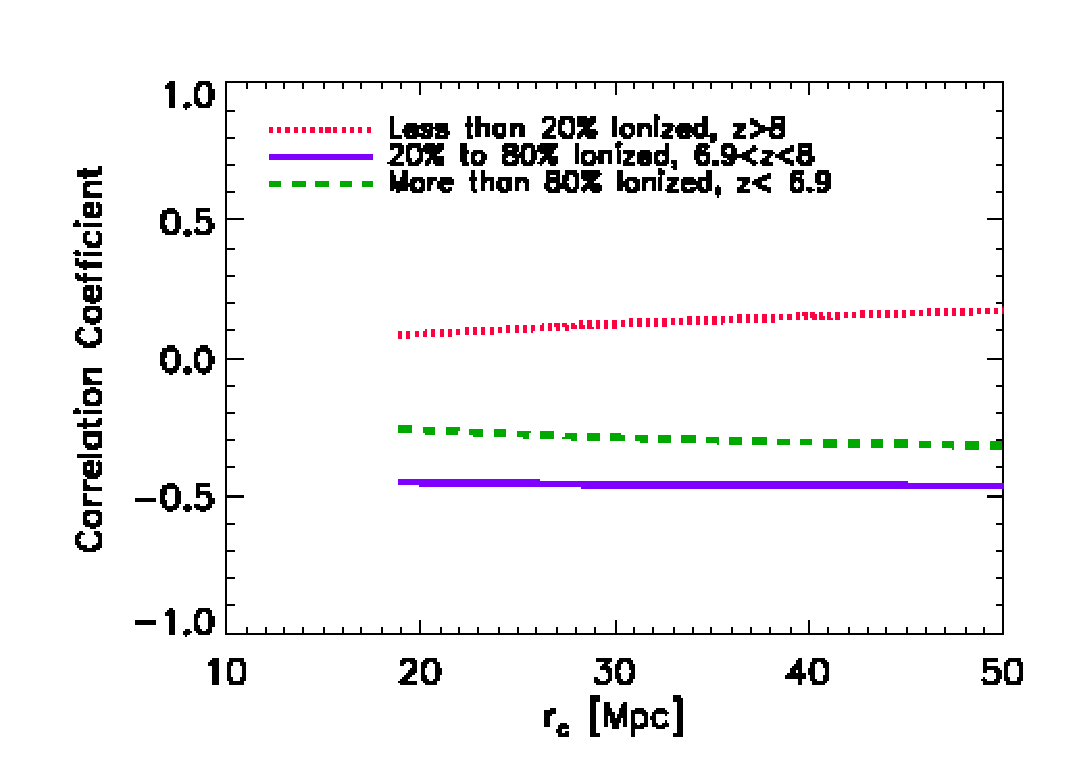
\includegraphics[width=70mm]{EoR/c03/c03.s2.f22.eps}
  \end{center}
 \end{minipage}
  \caption{$B6a@V30$H(B21~cm$BAj8_Aj4X78?t$X$N(BSKA$B$N46EY!J:8%Q%M%k!K$H%$%*%s2=(B
 $BN((B($B@VJ}JP0\(B)$B0MB8@-!J1&%Q%M%k!K!#(B}
  \label{fig:nirb_cross}
\end{figure}

$B1'Ch:F%$%*%s2=A0!"$b$7$/$O$=$N=i4|$K$O!"1'ChO@E*(B21~cm$B@~$N%7%0%J%k$NBg$-(B
$B$5$OL)EY$f$i$.$NBg$-$5$KHfNc$9$k!#6d2O$N?tL)EY$b$^$?L)EY$f$i$.$NBg$-$5$K(B
$BHfNc$9$k$?$a!"N><T$NAj8_Aj4X$O@5Aj4X$H$7$F8=$l$k!#(B
$B1'Ch$N:F%$%*%s2=$,?J$`$H!"1'ChO@E*(B21~cm$B@~$N%7%0%J%k$NBg$-$5$OCf@-?eAG$,(B
$B$I$l$[$I%$%*%s2=$5$l$:$K;D$5$l$F$$$k$+$K0MB8$9$k!#6d2O$O%$%*%s2=8w;R$N6!(B
$B5k8;$H$J$j$($k$N$G!"EvA3!"6d2O$N?tL)EY$,B?$$$H$3$m$G$O!"B?$/$N?eAG$,%$%*(B
$B%s2=$5$l$k$3$H$K$J$k!#$=$N$?$a!"%$%*%s2=$5$l$F$$$kNN0h!J%$%*%s2=%P%V%k!K$O!"(B21~cm$B@~$H6d2O(B
$B$NAj8_Aj4X$K$*$$$F$O!"Ii$NAj4X$H$7$F8=$l$k!#(B
$B$7$?$,$C$F!"Ii$NAj4X$N8=$l$k%9%1!<%k$N@VJ}JP0\$KBP$9$k?J2=$h$j!"%$%*%s2=%P%V(B
$B%k$N@.D9$r8+$k;v$,$G$-$k!#(B



$B?^(B~\ref{fig:galaxy_cross}$B$O:F%$%*%s2=$N%7%_%e%l!<%7%g%s$h$jF@$i$l$?(BEoR$B4|$NAj8_Aj(B
$B4X$N%Q%o!<%9%Z%/%H%k$r<($7$F$$$k(B~\citep{2013MNRAS.432.2615W}$B!#?^$N2<%Q%M(B
$B%k$r$_$k$H(B$z=9$$B$G(B$k \sim 0.3-0.4~h{\rm Mpc}^{-1}$$B$G8=$l$F$$$k(B
$BH?Aj4X$,:F%$%*%s2=$,?J$`$K$D$l$FBg$-$J%9%1!<%k$K0\F0$7$F$$$k!#(B
$B$7$?$,$C$F!"9b@VJ}JP0\6d2O$H(B21~cm$B@~$NAj8_Aj4X$r$H$l$P!"(B
$B$=$l$>$l$N@VJ}JP0\$G$NE57?E*$J%P%V%k%5%$%:$K%"%/%;%9$G$-$k2DG=@-$,$"$k;v(B
$B$,$o$+$k!#(B





\subsubsection{NIRB$B$H$NAj8_Aj4X(B}


$B1'Ch=i4|$N6d2O$d@1!9$O!"1'Ch:F%$%*%s2=$N$?$a$NM-8z$J%$%*%s2=8w;R6!5k8;$G(B
$B$"$k!#$7$?$,$C$F!"9b@VJ}JP0\$N@17A@.;K$rM}2r$9$k;v$O!"1'Ch:F%$%*%s2=;K$X$NM}2r$X$H$D$J$,$k!#(B
$B8=:_$N4QB,$K0M$l$P!"1'Ch$N:F%$%*%s2=$N$?$a$K$O8=:_4QB,$5$l$F$$$k6d2O$d@1!9(B
$B$h$j$b$5$i$KB?$/$N0E$/$F4QB,$5$l$F$$$J$$6d2O$d@1$,I,MW$G$"$k$3$H$,L@$i$+(B
$B$K$5$l$?!#$3$l$i$N@1$O2D;k8w$G$O4QB,$9$k$K$O0E$/$F$b!"@V(B
$BJ}JP0\$N7k2L!"6a@V30@~$GGX7JJ|<M$N0lIt$H$7$F51$$$F$$$k$3$H$,4|BT$5$l$F$$$k!#(B
$B$=$N$?$a!"6a@V30@~$NGX7JJ|<M$N4QB,$O!"1'Ch=i4|$N@1$N7A@.N($d$=$NJ,I[$NM}(B
$B2r$N=EMW$J%-!<$G$"$k(B~($B4XO"%l%S%e!<$H$7$F!"Nc$($P(B
\cite{2005PhR...409..361K}$B$r8+$h(B)$B!#(B


$B$9$G$K2?EY$b=R$Y$F$$$k$h$&$K!"(BEoR$B$+$i$N1'ChO@E*(B21~cm$B@~$N%7%0%J%k$N6/$5$O!"Cf@-?e(B
$BAG$NL)EY$K0MB8$7$F$$$k!#$9$J$o$A!"$=$N%7%0%J%k$N6/$$NN0h$O@1$d6d2O$,>/(B
$B$J$/!"?eAG$,%$%*%s2=$5$l$:$K<h$j;D$5$l$F$$$kNN0h$G$"$k!#(B
$BEvA3!"$=$NNN0h$O@1$d6d2O$,>/$J$$$N$G!"6a@V30@~$G8+$k$H0E$$!#(B
$B5U$K8@$($P!"6a@V30@~$G$_$FL@$k$$NN0h$O!"%$%*%s2=8w;R6!5k8;$G$"$k6d2O$d@1(B
$B$,B?$$NN0h$J$N$G!"1'ChO@E*(B21~cm$B@~$N%7%0%J%k$O<e$/$J$k!#(B
$B$D$^$j!"1'ChO@E*(B21~cm$B@~$H(BNIRB$B$N6/$5$OH?Aj4X$N4X78$K$"$k(B~\citep{2014MNRAS.440..298F}$B!#(B

\cite{2014MNRAS.440..298F}$B$O1'Ch=i4|$N6d2O(B
$B$K$h$k:F%$%*%s2=$N%7%_%e%l!<%7%g%s$r9T$$!"1'ChO@E*(B21~cm$B@~$H(BNIRB$B$NAj8_Aj(B
$B4X$r5a$a$?!#?^(B~\ref{fig:nirb_cross}$B$N:8%Q%M%k$,<($9$h$&$K!":F%$%*%s2=$N(B
$B?J9T$H$H$b$KH?Aj4X$N%7%0%J%k$OBg$-$/$J$j!"1'Ch$NBgH>$,:F%$%*%s2=$5$l$k$H(B
$B$=$N%7%0%J%k$O>.$5$/$J$C$F$$$/!#?^(B~\ref{fig:nirb_cross}$B$N1&%Q%M%k$O(B
$6 < z < 30$$B$+$i$N(BNIRB$B$H(B$6.4 < z < 11.1$$B$+$i$N(B21~cm$B@~$H$NAj8_Aj4X$rI=$7(B
$B$F$$$k!#$3$N?^$N%(%i!<%P!<$O(BLOFAR$B$N46EY$K4p$E$$$?$b$N$G$"$j!"(BSKA$B$G$O99$K(B
$B>.$5$$%(%i!<%P!<$,4|BT$5$l$F$$$k!#(B
%宇宙論的観測と中性水素21~cm線の相互相関
\subsection{$BJ?6Q%7%0%J%k(B}\label{c03.s3.ss1}
$B@VJ}JP0\$7$?(B21cm$B@~$rA4E7$KOJ$C$F4QB,$9$k$3$H$K$h$j!"J?6QE*$J1'Ch$NG.;K$r(B
$BCN$k$3$H$,$G$-$k$H4|BT$5$l$F$$$k!#FC$K:F%$%*%s2=$N%7%0%J%k(B
$B!J(BLyman-$\alpha$$B@~(B$\cdot$X$B@~$N8z$-;O$a$H8wNL!":FEEN%$N3+;O;~4|$H4|4V!"I8(B
$B=`%b%G%k$r1[$($?2CG.8;$NM-L5!K$O(BSKA-low (40GHz-200MHz)$B!"@2$l>e$,$j;~$N:F(B
$B7k9g@~$O(BSKA-mid$B$G$N%?!<%2%C%H$H$J$C$F$$$k!#(B

$BA4E7$N4QB,$K$D$$$F$O!"(BSKA$B$N$h$&$JBg5,LO$J43>D7W%7%9%F%`$O86M}E*$K$OI,MW$G(B
$B$O$J$/!"4{$K(Bsystematic dominated$B$J4QB,$K$J$C$F$*$j!"<B:]$K(BCoRE, EDGES,
LEDA, DARE, SARAS, SCI-HI, ZEBRA$B$J$I$N4QB,$,<B;\(B$\cdot$$B7W2h$5$l$F$$$k!#:G(B
$B?7$N4QB,$N0lNc$H$7$F(BSCI-HI$B$K$h$k7k2L$r<($9(B \citep{2014ApJ...782L...9V}$B!#(B
$B?^(B(\ref{fig:ichiki.fig.1})$B$NNP?'$K$h$k%G!<%?$,(B Global Sky Model
\citep{2008MNRAS.388..247D}$B$K$h$C$F(B 
$BA07JJ|<M$r?dDj$7:9$70z$$$?7k2L$N%Q%o!<$G$"$j!"@~$O:F%$%*%s2=%7%0%J%k$N(B
$B%b%G%k7W;;(B (3$B<oN`(B) $B$G$"$k!#$3$3$G$N<g$J7OE}8m:9$OA07JJ|<M$N:9$70z$-$N;D(B
$B:9$*$h$S%"%s%F%J%7%9%F%`$N<+8JL5@~<~GHK832(B (RFI)$B$G$"$k(B
$B$H5DO@$5$l$F$$$k(B \citep{2014ApJ...782L...9V}$B!#(B

\begin{figure}[!t]
\begin{minipage}[c]{0.49\linewidth}
\centering
{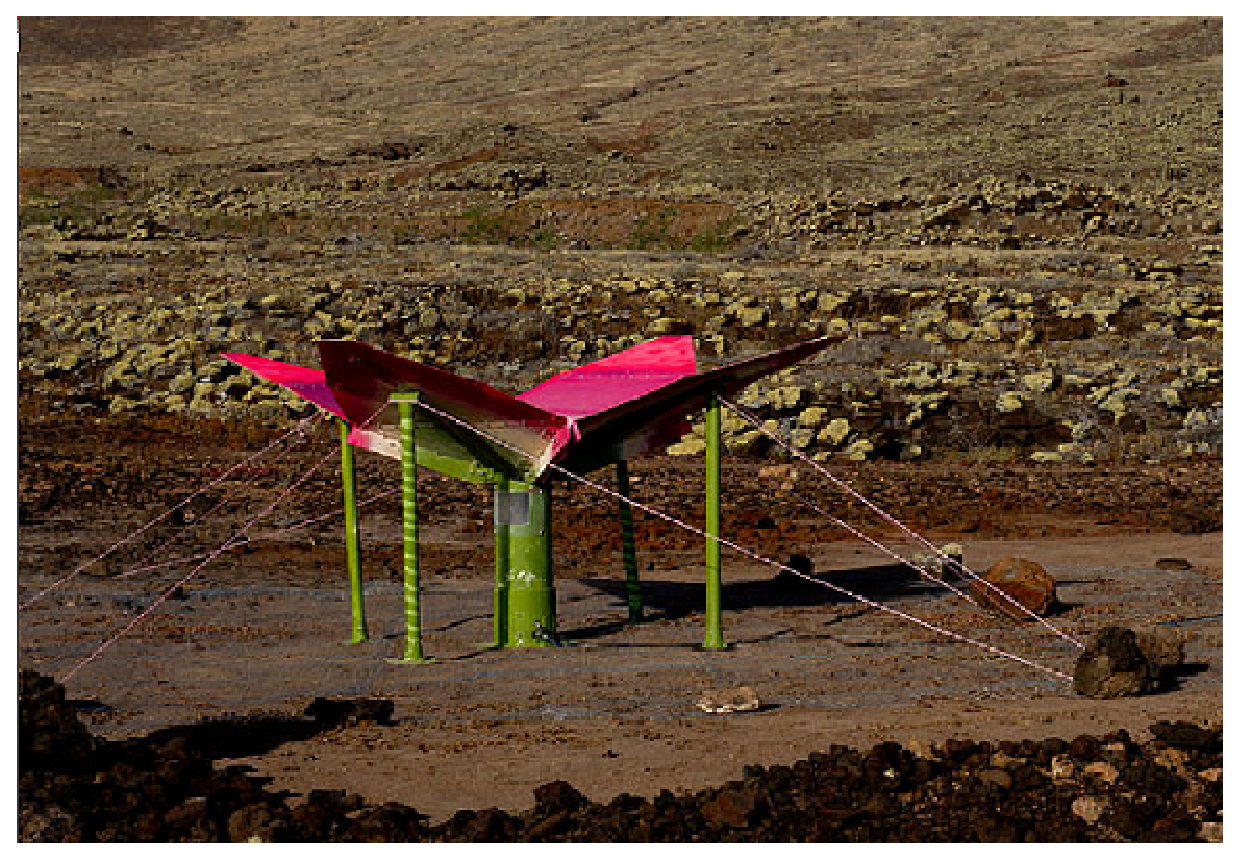
\includegraphics[width=\linewidth]{EoR/c03/c03.s2.f23.eps}}
\end{minipage}
\begin{minipage}[c]{0.49\linewidth}
\centering
{\includegraphics[width=\linewidth]{EoR/c03/c03.s2.f24.eps}}
\end{minipage}
\caption{Sonda Cosmologica de las Islas para la Deteccion de Hidrogeno
 Neutro (SCI-HI) $B$K$h$k4QB,Nc(B \citep{2014ApJ...782L...9V}$B!#(B}
\label{fig:ichiki.fig.1}
\end{figure}

$B$5$F!"$G$O$J$<43>D7W%7%9%F%`$G$"$k(BSKA$B$NK>1s6@$GE7$NJ?6QE*$J%7%0%J%k$,4QB,(B
$BBP>]$H$J$k$N$@$m$&$+!)$3$l$K$D$$$F$O43>D7W%7%9%F%`$r43>D7W$H$7$FMQ$$$:4Q(B
$BB,$9$kMxE@$H$7$F0J2<$N$h$&$J5DO@$,$"$k!#(B
\begin{itemize}
 \item $BA4E7%7%0%J%k4QB,$N:GBg$N7OE}8m:9$O%b!<%I%+%C%W%j%s%0!J<~GH?tKh$N(B
       $B%S!<%`$N0c$$$K$h$C$F6u4VJ}8~$NMI$i$.$,<~GH?tJ}8~$NMI$i$.$H:.$6$k!K(B
       $B$G$"$j!"$3$l$r<h(B
       $B$j=|$/<jK!$H$7$F(BSKA$B$N43>D7W%b!<%I$,M-8z!#(B
 \item $B43>D7W%7%9%F%`$K$h$k>\:Y4QB,$r9T$&%?!<%2%C%H@VJ}JP0\$r$^$:J?6Q%7(B
       $B%0%J%k$+$iC5$k!#(B
 \item $B29EY$N%<%mE@$rB,$k!J43>D7W%b!<%I$GF@$i$l$?%Q%o!<%9%Z%/%H%k$O5[<}(B
       $B$K$h$k$b$N$J$N$+!"J|<M$J$N$+!K!#(B
\end{itemize}
SKA$B$r$I$N$h$&$KMQ$$$k$+$K$D$$$F$OBg$-$/J,$1$FFsDL$j$,9M$($i$l$F$$$k!#$9(B
$B$J$o$A!"D>7B(B $35$ m$B$N(Bstation$B$r0l$D$NK>1s6@$H$7$FMQ$$$kJ}K!$G!";kLn$,(B
$5\times 5$ $BJ?J}EY$HHf3SE*69$/$J$k$?$aA07JJ|<M$N:9$70z$-$O$7$d$9$/$J$k$,!"(B
$B%b!<%I%+%C%W%j%s%0$,J#;($K$J$k!#$^$?$O(Bstation$B$K$"$k0l$D$N%"%s%F%J$@$1$r(B
$BK>1s6@$H$7$FMQ(B
$B$$$kJ}K!$G!"$3$N>l9g$O%b!<%I%+%C%W%j%s%0$O8:$k$b$N$N!";kLn$,(B$90\times 90$$BJ?J}EY(B
$B$H9-$/$J$jA07JJ|<M$N:9$70z$-$OFq$7$/$J$k!#(B

$B$^$?!"43>D7W$O0lHL$KA4E7$NJ?6Q(Bsignal$B$K$O46EY$,$J$$$,!"?)$r5/$3$7$F$$$kE7BN(B
$B!JNc$($P7n!K$,$"$l$P!"$N$C$Z$j$7$?A4E7%7%0%J%k$K6u4VE*$J9=B$$,@8$8$k$3$H(B
$B$K$J$j4QB,$,2DG=$H$J$k!#FC$K!"7n$O$[$\0lMM$J(B$230$K$B$N9uBNmU<M$@$H4|BT$5$l$F(B
$B$$$k$N$G!"$3$l$r4p=`$KA4E7%7%0%J%k$rB,$k$3$H$,$G$-$k!#<B:](BLOFAR$B$K$h$k<B(B
$B83$K$h$j!"LdBj$K$J$k$H;W$o$l$F$$$?CO5e$N(BRFI$BH?<MGH$OD94p@~(B ($\gtrsim
100\lambda$) $B4QB,$K$h$j%b%G%k2=$7:9$70z$1$=$&(B
$B$G$"$k$3$H!"(BSKA$BDxEY$N(Bfilling factor$B$,$"$l$P?tF|$N4QB,;~4V$G8!=P2DG=$G$"(B
$B$k$3$H$,L@$i$+$K$5$l$F$$$k!#(B

%平均シグナル

